\documentclass{tnreport}
%\documentclass[stage2a]{tnreport} % If you are in 2nd year
%\documentclass[confidential]{tnreport} % If you are writing confidential report

\def\reportTitle{
	Implémentation d’un service de liste de confiance globale basé sur la blockchain
	%Implémentation d’une Global Trust Service Status List basé sur la blockchain
	%Implémentation d'une liste globale des services de confiance basée sur la blockchain
	%Implémentation d'une liste mondiale de confiance basée sur la blockchain
} % Titre du mémoire
\def\reportLongTitle{
	Implémentation d’un service de liste de confiance globale basé sur la blockchain
	%Implémentation d’un service de trust list global basé sur la blockchain
	%Implémentation d'un service de liste globale des services de confiance basé sur la blockchain
} % Titre plus long du mémoire

\def\reportAuthor{Yoann Raucoules}
\def\reportAuthorEmail{\email{yoann.raucoules@telecomnancy.eu}} % Courriel de l'élève

\def\reportAuthorAddress{6, rue du général Frère} % Adresse de l'élève
\def\reportAuthorCity{57070, METZ} % Adresse (cont.) de l'élève
\def\reportAuthorPhone{+33 (0)6 77 48 04 38} % Téléphone de l'élève 

\def\reportIndustrialSupervisor{Vincent Bouckaert} % Prénom Nom de l'encadrant industriel
\def\reportAcademicSupervisor{Olivier Festor} % Prénom Nom de l'encadrant académique

\def\reportCompany{ARHS Spikeseed} % Nom de l'entreprise d'accueil
\def\reportCompanyAddress{2B, rue Nicolas Bové}  % Adresse de l'entreprise
\def\reportCompanyCity{1253, LUXEMBOURG} % Adresse (cont.) de l'entreprise
\def\reportCompanyPhone{+352 26 11 02 1} % Téléphone de l'entreprise
\def\reportCompanyLogoPath{figures/logo-arhs-spikeseed} % Logo de l'entreprise -- comment this definition to remove company logo

\def\place{Luxembourg} % Ville pour la signature pour l'engagement anti-plagiat
\def\date{\today} % Date pour la signature de l'engagement anti-plagiat

\usepackage{textgreek}
\usepackage{pdfpages}
\usepackage{listings}

\colorlet{punct}{red!60!black}
\definecolor{background}{HTML}{EEEEEE}
\definecolor{delim}{RGB}{20,105,176}
\colorlet{numb}{magenta!60!black}

\lstdefinelanguage{solidity}{
	basicstyle=\normalfont\ttfamily,
	numbers=left,
	numberstyle=\scriptsize,
	stepnumber=1,
	numbersep=8pt,
	showstringspaces=false,
	keywords = [1]{contract, struct, mapping, public, for, import, private, event, function, if, else, delete, return, returns, enum, bytes32, bytes, uint},
	keywordstyle=[1]\color{blue},
	breaklines=true,
	frame=lines,
	backgroundcolor=\color{background},
	comment=[l]{//},
	morecomment=[s]{/*}{*/},
	commentstyle=\color{purple}\ttfamily,
}

\lstdefinelanguage{json}{
	basicstyle=\normalfont\ttfamily,
	numbers=left,
	numberstyle=\scriptsize,
	stepnumber=1,
	numbersep=8pt,
	showstringspaces=false,
	breaklines=true,
	frame=lines,
	backgroundcolor=\color{background},
	literate=
	*{0}{{{\color{numb}0}}}{1}
	{1}{{{\color{numb}1}}}{1}
	{2}{{{\color{numb}2}}}{1}
	{3}{{{\color{numb}3}}}{1}
	{4}{{{\color{numb}4}}}{1}
	{5}{{{\color{numb}5}}}{1}
	{6}{{{\color{numb}6}}}{1}
	{7}{{{\color{numb}7}}}{1}
	{8}{{{\color{numb}8}}}{1}
	{9}{{{\color{numb}9}}}{1}
	{:}{{{\color{punct}{:}}}}{1}
	{,}{{{\color{punct}{,}}}}{1}
	{\{}{{{\color{delim}{\{}}}}{1}
	{\}}{{{\color{delim}{\}}}}}{1}
	{[}{{{\color{delim}{[}}}}{1}
	{]}{{{\color{delim}{]}}}}{1},
}

\begin{document}
  
\maketitle
\pagenumbering{roman}

\insertAntiPlagiarismAgreement{Raucoules, Yoann}{1205028998}

\cleardoublepage

\makesecondtitle

\section*{Remerciements}
\addcontentsline{toc}{chapter}{Remerciements}

Je tiens tout d'abord à remercier Madame Carlyne BALCZESAK, Monsieur Sébastien BRAUN et Monsieur Christophe GROSJEAN qui m'ont permis d'intégrer les équipes d'Ar{\texteta}s pendant ces six mois de stage. 

Je tiens également à remercier et à témoigner toute ma reconnaissance à mon maître de stage Monsieur Vincent BOUCKAERT pour cette expérience enrichissante et pleine d’intérêt, pour le temps qu’il m'a consacré tout au long de ce stage en répondant à mes interrogations. 

Je souhaite aussi remercier Thomas LOISE et Francisco ROCHA qui ont contribué à ce projet et qui m'ont notamment aidé pour la rédaction de ce mémoire. 

J'adresse aussi mes remerciements à l'ensemble des collaborateurs d'Ar{\texteta}s qui par leur accueil et leur sympathie m'ont permis d'évoluer en toute sérénité au sein de l'entreprise. 

Enfin, je tiens à remercier mon encadrant universitaire Monsieur Olivier FESTOR pour son intérêt porté au projet, son implication, son suivi tout au long de ce stage ainsi que pour sa visite dans les locaux de l'entreprise.

\cleardoublepage

\section*{Avant-propos}
\addcontentsline{toc}{chapter}{Avant-propos}

Ce mémoire résulte d'un stage de fin d'études qui s'est déroulé du 3 avril 2017 au 30 septembre 2017 au sein de l'entreprise Ar{\texteta}s Spikeseed située au Luxembourg. Ce stage vient clôturer et valider la formation d'ingénieur du numérique de l'école TELECOM Nancy que j'ai débutée en septembre 2014. Cette formation qui s'est étendue sur une période de trois ans m'a permis d'acquérir de nombreuses compétences dans les domaines de l'informatique, des mathématiques, du management, de la gestion de projet, de la communication, de l'économie, du droit et des langues. J'ai choisi de me spécialiser en Ingénierie Logicielle au cours du cursus de par ma passion pour la programmation et l'architecture logicielle qui s'est révélée lorsque je me suis initié à l'informatique lors de mon stage de découverte professionnelle réalisé en classe de troisième.

Au cours de ce stage de fin d'études, j'ai eu le plaisir de travailler sur une technologie à laquelle je m'intéresse depuis deux ans, la blockchain. Dans le cadre d'un projet proposé par la Commission Européenne, nommé FutureTrust, j'ai pu concevoir et implémenter un service de liste de confiance globale basé sur la blockchain. Mes tâches ont été de me familiariser avec les principes de la blockchain et les concepts de cryptographie afin de les mettre en application dans le projet, d'effectuer une analyse des solutions de blockchain existantes afin de réaliser des choix d'implémentation, de concevoir l'architecture du service de liste de confiance globale, d'implémenter la solution conçue et de documenter tous les aspects techniques et fonctionnels de la solution implémentée.

Dans ce mémoire est présenté le résultat du stage de fin d'études et est mis en avant l'utilisation de la blockchain dans le cadre d'un projet de confiance numérique d'échelle mondiale. L'intérêt de ce document est dans un premier temps de détailler les tâches réalisées au cours du stage et dans un second temps de montrer qu'il est possible d'élargir le champ d'application de la technologie blockchain et des différents aspects qui la composent.

\cleardoublepage

\renewcommand{\baselinestretch}{0.5}\normalsize
\tableofcontents
\renewcommand{\baselinestretch}{1.0}\normalsize
\cleardoublepage

\pagenumbering{arabic}
\setcounter{page}{1}

\chapter{Introduction}

La technologie blockchain s'est popularisée ces dernières années grâce à l'expansion de la crypto-monnaie\footnote{La crypto-monnaie aussi appelée monnaie cryptographique est une monnaie électronique basée sur les principes de la cryptographie.} Bitcoin\footnote{Bitcoin est une crypto-monnaie et un système de paiement pair-à-pair.}~\cite{Bitcoin} à travers le monde. 
En effet, cette technologie a bouleversé aussi bien le domaine de l'informatique que le domaine de la finance. 
L'investissement autour de la blockchain a mené à un engouement général pour ce concept. 
Le Bitcoin a réussi à remettre en cause des acteurs majeurs de notre société tels que les banques ou les géants du Web, en sécurisant des échanges d'actifs sans organe central de contrôle. 
La révolution qu'il a engendrée amène aujourd'hui les gouvernements et autres organisations publiques à réfléchir sur la régulation de la technologie et des crypto-monnaies naissantes.
Depuis son lancement en 2009, la blockchain n'a cessé d'évoluer et d'étendre son champ d'application.
Bien que conçue à l'origine pour le transfert de crypto-monnaie, les avantages qu'elle apporte permettent d'imaginer de multiples cas d'utilisation qui dépassent son cadre initial.
À l'heure où l'ubérisation\footnote{L'ubérisation est un phénomène économique désignant l'utilisation de services permettant aux professionnels et aux clients de se mettre en contact direct grâce à l'utilisation des nouvelles technologies.} de notre société est en marche, la technologie blockchain amène une approche nouvelle qui permet de se détacher de tout organe central ou tierce partie. 
La blockchain ira-t-elle jusqu'à ubériser\footnote{Ubériser est le verbe issu du substantif ubérisation.} Uber\footnote{Uber est l'entreprise qui déclencha l'ubérisation.} ?

%\section{Définition du cadre et des objectifs du stage}

Dans ce contexte, un stage ingénieur a été réalisé sur une période de six mois au sein de la société Arηs Spikeseed située au Luxembourg. 
Le stage a été réalisé dans les locaux de l'entreprise et la langue officielle du projet pour les communications avec les autres membres du consortium (mails, documents, conférences téléphoniques) a été l’anglais. La langue utilisée au sein de l'équipe a aussi été l'anglais, ceci étant dû au caractère multinational de celle-ci. Les documents produits dans le cadre du projet ont été rédigés en anglais et sont présentés en langue originale dans ce mémoire.
Ce stage de fin d'études a eu pour objectif d'intégrer la technologie blockchain au sein d'un processus de gestion de listes de services de confiance dans le cadre de la mise en place d'un nouveau règlement européen. 
La finalité a été d'utiliser cette technologie afin de conserver des données publiques relatives à la confiance électronique de manière sécurisée et décentralisée en utilisant une blockchain en tant que registre.
Cela a pour but d'assurer la disponibilité et l'intégrité des informations, puisque les données sont distribuées à travers les nœuds d'un réseau pair-à-pair et sécurisées à l'aide de transactions signées et vérifiées par une preuve mathématique. 

%\section{Mise en exergue du plan}

Ce mémoire vise à montrer que le champ d'application de la technologie blockchain dépasse son cadre initial et que son utilisation permet de pallier aux problèmes d'architecture et de sécurité des modèles actuels. 
Dans un premier temps, le contexte du stage sera défini afin de présenter l'entreprise Ar{\texteta}s Spikeseed, d'établir le contexte du projet et de détailler le fonctionnement de la technologie blockchain.
Ensuite, la problématique sera exposée dans le but de comprendre les différents besoins autour du service de liste de confiance globale et les limites de l'architecture actuelle. Ce chapitre détaillera aussi la méthodologie de gestion de projet ainsi que l'organisation du temps au cours du stage.
À la suite de cela, sera établi un état de l'art afin d'analyser l'émergence de la blockchain et l'intérêt porté aux systèmes décentralisés. Dans ce chapitre, la comparaison des outils existants et la justification des choix opérés durant le stage seront mises en évidence. 
Après cela, une analyse du problème sera développée en exposant les technologies utilisées, les acteurs du système, les cas d'utilisation de l'application ainsi que les modules, processus et modèle de données du service de liste de confiance globale.
Puis, la réalisation de la solution sera détaillée en mettant en avant l'architecture mise en place, l'implémentation des différents modules ainsi que la présentation et la validation de la solution.
Enfin, les résultats obtenus et les perspectives du projet seront présentés.

\chapter{Présentation du contexte}

Dans ce chapitre, nous présentons l'entreprise qui m'a accueilli dans le cadre de ce stage, le contexte dans lequel s'inscrit le projet réalisé ainsi qu'une introduction à la technologie blockchain.

\section{L'entreprise Ar{\texteta}s Spikeseed}

Ar{\texteta}s Spikeseed est une entité du groupe Ar{\texteta}s qui est une entreprise de services du numérique (ESN) fondée en 2003 par Jourdan Serderidis. 
Le groupe est divisé en sociétés réparties au Luxembourg, en Belgique, en Grèce et depuis cette année en Italie. Le groupe Ar{\texteta}s possède cinq axes de compétences qui sont présentés dans la Figure~\ref{fig:arhs-core-services}.

\begin{figure}[h]
	\centering
	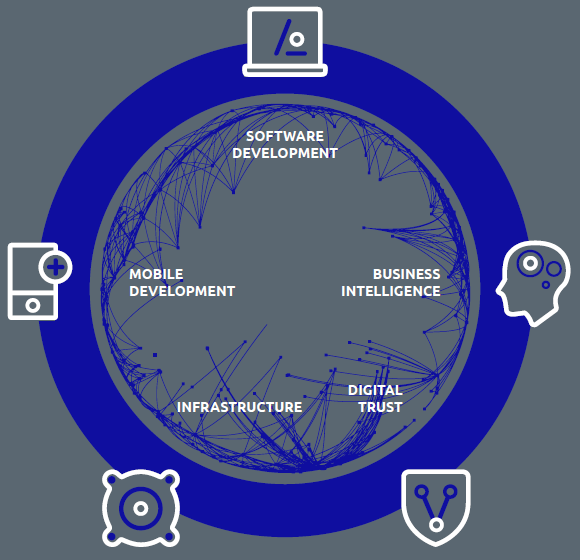
\includegraphics[scale=0.7]{figures/arhs-core-services}
	\caption{Axes de compétences du groupe Ar{\texteta}s. Illustration extraite de \textit{Annual Report 2016}~\cite{annual-report}}
	\label{fig:arhs-core-services}
\end{figure}

Comme toutes les autres entités du groupe, Ar{\texteta}s Spikeseed vise à délivrer des solutions numériques complexes. Elle a la particularité de réaliser principalement des projets de recherche et développement en s'appuyant sur les pratiques agiles et des technologies de pointe. 
De plus, l'entreprise Ar{\texteta}s Spikeseed est compétente pour mettre en œuvre 
des solutions liées à la confiance numérique, 
des systèmes engageant des masses de données ainsi que 
des applications destinées aux mobiles et aux objets connectés.

\section{Contexte du projet}

Les architectures logicielles évoluent en suivant les innovations technologiques. Le domaine de la recherche apporte de nouvelles technologies et des améliorations aux concepts existants à une vitesse exponentielle. L'univers technologique poussé par l'innovation oblige les acteurs du numérique à s'adapter en permanence aux changements. La technologie blockchain s'inscrit dans ces innovations récentes issues de la recherche. Elle amène une nouvelle vision d'un Internet décentralisé, sans organe central de contrôle, qui va probablement révolutionner la conception des systèmes d'information dans les prochaines années.

Dans le cadre de la mise en place d'un règlement de l'Union Européenne (UE) sur l'identification électronique et les services de confiance pour les transactions électroniques sécurisées au sein de l'UE (eIDAS), la Commission Européenne (CE) a proposé un projet qui a pour objectif de supporter la mise en œuvre technique de ce règlement européen. 
Le règlement eIDAS~\cite{eIDAS} a pour but d'établir un cadre d’interopérabilité pour les systèmes mis en place au sein de l'UE afin de promouvoir le développement d’un marché de la confiance numérique, et d'instaurer un mécanisme de reconnaissance mutuelle des moyens d’identification électronique des États membres sur l’ensemble des services fournis par d'autres États membres.

Ce projet de recherche et développement appelé FutureTrust rassemble un consortium de seize partenaires, dont Ar{\texteta}s Spikeseed. 
Le projet FutureTrust répondra au besoin de solutions globales et interopérables, en fournissant des logiciels libres qui faciliteront l'utilisation de l'identification et de la signature électronique. 
Il vise à étendre l'infrastructure de la liste européenne de services de confiance existante vers une liste mondiale des services de confiance nommée Global Trust Service Status List (gTSL), à développer un service de validation ainsi qu'un service d'archivage pour les signatures et les sceaux électroniques, et à fournir des composants pour les certificats qualifiés et pour la création de signatures et de sceaux dans un environnement mobile.

Dans ce contexte, l'intégration de la blockchain a été proposée dans le cadre du projet FutureTrust et plus particulièrement dans le module de gTSL. Les autres modules du projet n'entrent pas dans le cadre du stage et ne sont pas détaillés dans ce document. 

\section{Présentation de la technologie blockchain}

Une blockchain est une technologie basée sur l'échange d'actifs numériques réalisé grâce à des transactions signées, et agit comme un registre public distribué où toutes les transactions émises sont répertoriées. Elle repose sur des principes de cryptographie afin d'assurer l'intégrité de ces transactions et sur un protocole décentralisé, dit "peer-to-peer". Ce protocole permet à la blockchain d'avoir une disponibilité maximale et d'établir un consensus entre les participants du réseau afin de protéger les transactions contre les falsifications. La Figure~\ref{fig:blockchain-diagram} représente le processus d'émission et de validation d'une transaction sur la blockchain.

\begin{figure}[h]
	\centering
	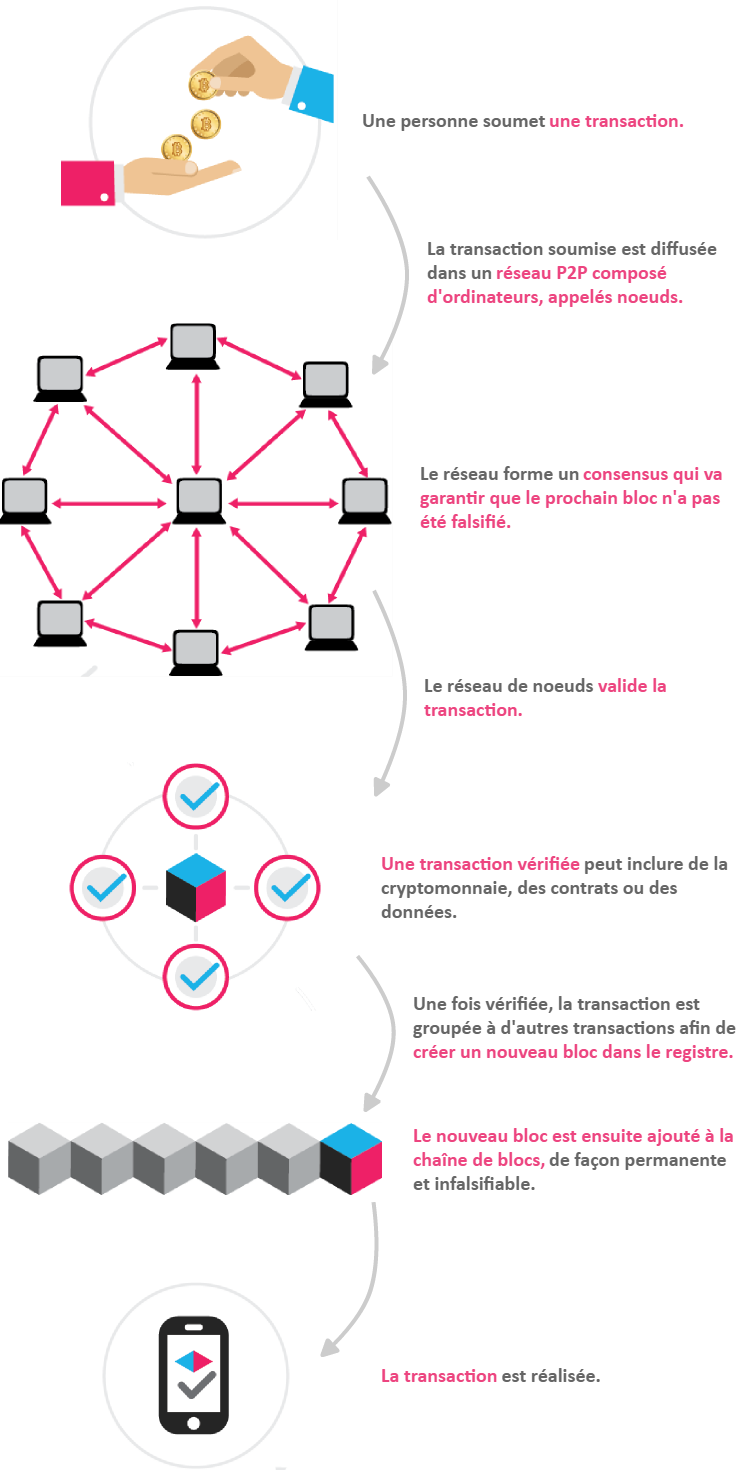
\includegraphics[scale=0.45]{figures/blockchain-diagram}
	\caption{Processus de création et de validation d'une transaction sur la blockchain. Illustration adaptée de \textit{What is Blockchain Technology ?}~\cite{blockchain}}
	\label{fig:blockchain-diagram}
\end{figure}
\clearpage

Dans la Figure~\ref{fig:blockchain-diagram}, nous remarquons que les blocs sont agencés dans un ordre linéaire, à la manière de maillons dans une chaîne, et contiennent une référence au bloc précédent, ainsi qu'un enregistrement des transactions.
La preuve de travail est le traitement nécessaire pour générer un nouveau bloc basé sur les nouvelles transactions diffusées sur le réseau.
Les blocs de transaction sont créés par un processus appelé le minage\footnote{mining en anglais.}, qui est conçu pour être coûteux en temps et en énergie ainsi qu'être complexe à réaliser, et s'appuie sur un consensus pour ajuster la difficulté de créer de nouveaux blocs. Le minage est aussi un moyen de sécuriser le réseau en créant, vérifiant, publiant et propageant les blocs dans la blockchain.

\subsection{Introduction aux Smart Contracts}

En 1994, Nick Szabo, chercheur juridique et cryptographe, s'est rendu compte que le registre décentralisé pouvait être utilisé pour des smart contracts (contrats intelligents), autrement appelés contrats auto-exécutés, contrats blockchain ou contrats numériques.
Les contrats peuvent être convertis en code informatique, stockés et répliqués sur le système.
Les smart contracts permettent d'échanger de l'argent, des biens, des parts ou n'importe quel actif de manière transparente, sans conflits et en évitant tout service intermédiaire.
La Figure~\ref{fig:smart-contracts} représente l'établissement d'un smart-contract entre deux parties, sans service intermédiaire. Dans ce mémoire, nous utilisons le terme de smart contract pour désigner un contrat intelligent car ce terme est le plus répandu.

\begin{figure}[h]
	\centering
	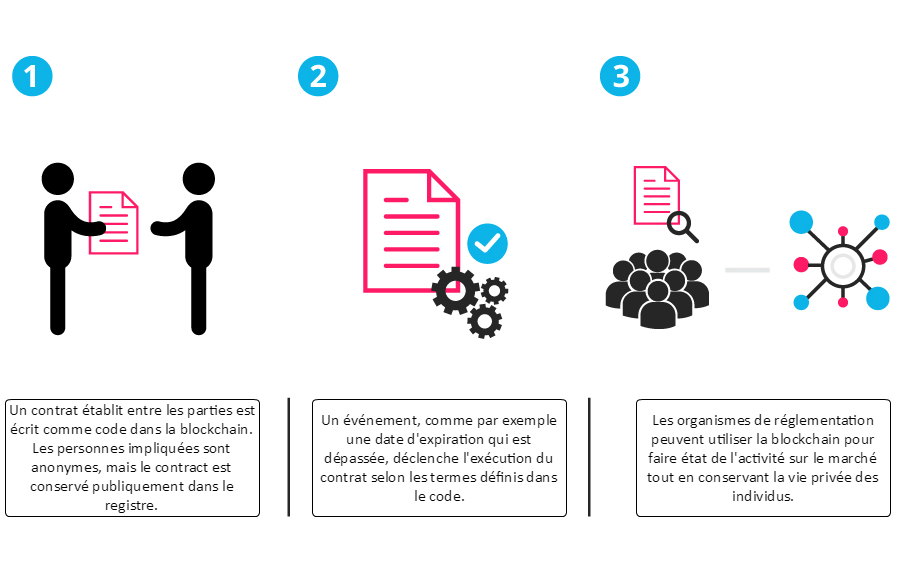
\includegraphics[scale=0.53]{figures/smart-contracts}
	\caption{Établissement d'un smart-contract. Illustration adaptée de \textit{Smart Contracts: The Blockchain Technology That Will Replace Lawyers}~\cite{smart-contracts}}
	\label{fig:smart-contracts}
\end{figure}

\clearpage
Les smart-contracts apportent de nombreux avantages pour leurs utilisateurs:
\begin{itemize}
	\item l'autonomie, qui signifie que l'accord engendré par le contrat n'a pas besoin d'être confirmé par un intermédiaire comme un notaire ou un avocat;
	\item la confiance, puisque les documents sont encodés dans le registre distribué, il n'y a aucun moyen qu'ils soient perdus;
	\item la sauvegarde, toutes les informations sont stockées dans la blockchain et sont répliquées à travers de multiples nœuds du réseau qui les maintiennent;
	\item la sécurité, les concepts de cryptographie utilisés permettent de conserver les contrats en sécurité, ils ne peuvent être modifiés ou usurpés;
	\item la vitesse, les smart-contracts permettent d'accélérer les procédures, en effet toutes les tâches sont automatisées donc aucun tiers ne ralentit le processus;
	\item des économies, en effet se détacher des intermédiaires permet de réduire considérablement les charges administratives engendrées par la plupart des contrats classiques;
	\item la précision, puisque le contrat est automatisé et exécuté par une machine, si l'on admet que le contrat a été codé correctement, alors toute erreur pouvant être introduite lors d'une rédaction manuelle ne peut être présente dans un smart-contract.
\end{itemize}

\chapter{Présentation détaillée de la problématique}
\label{chap:prob}

Dans ce chapitre, nous présentons les besoins liés au service de liste de confiance globale ainsi que les limites de l'architecture actuelle. Ce chapitre introduit aussi les concepts relatifs à la gestion de projet, plus précisément la méthodologie utilisée et l'organisation du temps au cours du stage.

\section{Description des besoins du service de liste de confiance globale}
\label{sec:description}

Les États membres de l'UE et d'autres pays européens maintiennent généralement des listes d'informations sur des autorités de certification, ainsi que des listes d'informations sur des fournisseurs de services, désignés Trust Service Providers (TSP), dans un ou plusieurs registres à l'échelle nationale.

La liste de confiance des États membres de l'UE comprend des informations relatives aux TSPs qualifiés qui sont supervisés par l'État membre compétent, ainsi que des informations relatives aux services de confiance, désignés Trust Services (TS), qu'ils fournissent, conformément aux dispositions prévues par le règlement eIDAS.
En effet, les listes de confiance sont des éléments essentiels dans la mise en place de la confiance numérique pour les opérateurs du marché électronique, en permettant aux utilisateurs de déterminer le statut qualifié des TSPs et de leurs TSs.

En vertu du règlement eIDAS, les listes nationales de confiance ont un effet constitutif.
En d'autres termes, un fournisseur ou un service ne sera qualifié que s'il apparaît dans les listes de confiance. Par conséquent, les utilisateurs (citoyens, entreprises ou administrations publiques) bénéficieront de l'effet juridique associé à un service de confiance qualifié uniquement si ce dernier est répertorié (comme qualifié) dans les listes de confiance.	
Les États membres peuvent inclure dans les listes de confiance des informations sur les fournisseurs de services de confiance non qualifiés et sur d'autres services de confiance définis au niveau national.

La structure d'une liste de confiance est présentée dans la Figure~\ref{fig:tsl-scheme}.

\begin{figure}[h]
	\centering
	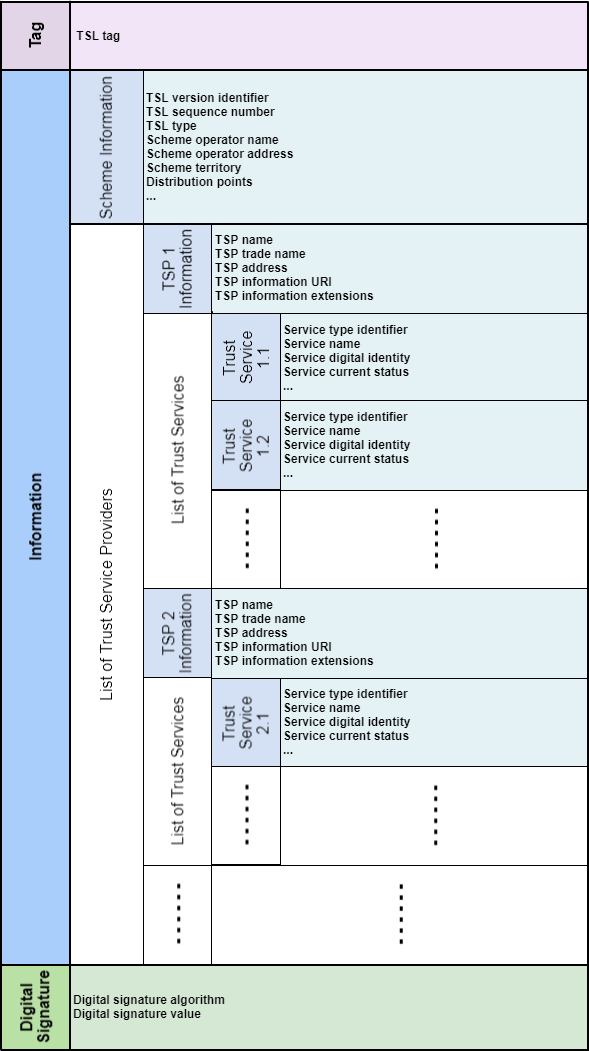
\includegraphics[scale=0.65]{figures/tsl-scheme}
	\caption{Structure d'une liste de confiance}
	\label{fig:tsl-scheme}
\end{figure}

\clearpage

Dans la Figure~\ref{fig:tsl-scheme}, on distingue qu'une liste de confiance peut être décomposée en trois sections. 

\subsubsection{Tag}

La section \textit{Tag}, et plus particulièrement son attribut \textit{TSL Tag}, est une URI\footnote{Une URI (acronyme anglais de Uniform Resource Identifier) est une chaîne de caractères identifiant une ressource.} qui permet d'indiquer le standard sur lequel s'appuie la liste de confiance. Actuellement, le seul standard  existant est ETSI TS 119 612~\cite{ETSITS119612}. Il est possible qu'un nouveau standard soit défini dans le futur, cette section permettra donc d'indiquer le standard sur lequel la liste de confiance est basée.

\subsubsection{Information}

La section \textit{Information} peut-être divisée en deux parties. 
La première partie, nommée \textit{Scheme Information}, répertorie toutes les informations relatives à la liste de confiance comme par exemple sa version, le nom et l'adresse de l'opérateur de la liste ou encore le pays pour lequel la liste est définie. Il est important de noter que dans la Figure~\ref{fig:tsl-scheme}, la liste des informations citées n'est pas exhaustive. 
La seconde partie est la liste des TSPs qui répertorie l'ensemble des fournisseurs approuvés par l'État membre. Pour chacun des TSPs, on retrouve ses informations ainsi que la liste des services de confiance qu'il fournit.

\subsubsection{Digital Signature}

La section \textit{Digital Signature} permet de vérifier l'authenticité et l'intégrité de la liste de confiance. En effet, chaque liste doit être signée par un opérateur désigné et défini dans la partie \textit{Scheme Information}. Dans cette section doivent être indiqués la signature de l'opérateur ainsi que l'algorithme de génération de celle-ci.

\subsection{Besoins généraux}

\subsubsection{Résumé des objectifs du projet}

L'intérêt du service de gTSL est de favoriser l'établissement de relations de confiance entre les opérateurs du marché en Europe et au-delà. Cette liste a pour but de répertorier les TSPs, ayant un statut qualifié ou non. 
Le statut qualifié signifie que le TSP a été accrédité par un organisme compétent au sein de l’État membre dans lequel il est déclaré. Le service permet aux utilisateurs finaux de vérifier le statut de ces TSPs et d'accéder à l'ensemble des informations concernant les services de confiance. À ce titre, la gTSL étend le schéma actuel de la liste des services de confiance, dont la portée est uniquement européenne. De plus, cette réorganisation de l'architecture vise à gérer la gTSL de manière décentralisée dans le but d'en améliorer sa résilience.

\subsubsection{Parties prenantes}

Les acteurs principaux de la gTSL sont:
\begin{itemize}
	\item les États membres de l'UE, qui doivent établir, maintenir et publier les listes de confiance, incluant les informations relatives aux TSPs déclarés au sein de leur État;
	\item les fournisseurs de services de confiance, qui s'appuient sur le service de gTSL dans lequel sont publiés leurs statuts qualifiés et leurs informations publiques;
	\item les opérateurs de listes de confiance ne faisant pas partie d'un État membre de l'UE, qui souhaitent intégrer leur liste dans la gTSL;
	\item les citoyens de l'UE et non UE, qui utilisent le service afin d'accéder aux statuts et aux informations des différents TSPs répertoriés dans la gTSL.
	\newline
\end{itemize}

\subsection{Besoins du système}
\label{sec:system-requirements}

\subsubsection{Objectif du système}

En s'appuyant sur la norme régissant les listes de confiance définie dans ETSI TS 119 612~\cite{ETSITS119612}, la gTSL vise à résoudre les imperfections actuelles du schéma de liste de confiance, énoncées dans la Section~\ref{sec:limits}. 

À l'heure actuelle, la Commission européenne publie une liste signée de pointeurs, nommée European List of the Lists (LoTL), dans laquelle chaque pointeur désigne un point de distribution pour une liste nationale de TSPs. 
Ces listes nationales contiennent des informations sur les TSPs qualifiés et non qualifiés ainsi que sur les TSs qualifiés ou non qualifiés qu'ils proposent.

À ce titre, la gTSL fournira les fonctions nécessaires à la création, à la mise à jour et à la distribution des TSPs et des informations concernant leurs TSs.
Le but principal de la gTSL est de s'appuyer sur le modèle centralisé actuel et de l'adapter à un nouveau modèle décentralisé.
L'émergence récente de la technologie blockchain ainsi que l'engouement général de la part de la communauté open-source autour de la décentralisation qu'elle rend possible nous apporte un contexte d'utilisation idéal dans notre objectif de décentralisation.

\subsubsection{Présentation du système}

Afin d'atteindre ses objectifs, la gTSL s'appuie sur quatre principaux composants:
\begin{itemize}	
	\item le \textit{Global Trust Service Responder}\footnote{en français, Répondeur (dans le sens où il répond aux requêtes des utilisateurs).} qui permet aux applications externes et aux utilisateurs d'interroger la gTSL afin de récupérer les informations relatives aux TSPs;
	\item l'interface d'administration qui a pour objectif de fournir une interface graphique ergonomique aux opérateurs afin qu'ils puissent facilement procéder à des modifications sur les listes de confiance;
	\item le \textit{Global Trust Service Lifecycle Manager}\footnote{en français, Gestionnaire du cycle de vie.} qui a pour vocation de faciliter la gestion des services de confiance à travers une interface permettant la création, la mise à jour et la distribution des informations relatives aux statuts de confiance;
	\item le \textit{Ledger Manager} qui a pour rôle de manipuler et de stocker les données.
	\newline
\end{itemize}
Ces composants et leurs interactions sont illustrés dans la Figure~\ref{fig:3tier-archi}.
%Les différents composants permettant de mettre en œuvre les fonctions de la gTSL sont présentés dans la Figure~\ref{fig:3tier-archi}.

\clearpage
\begin{figure}[h]
	\centering
	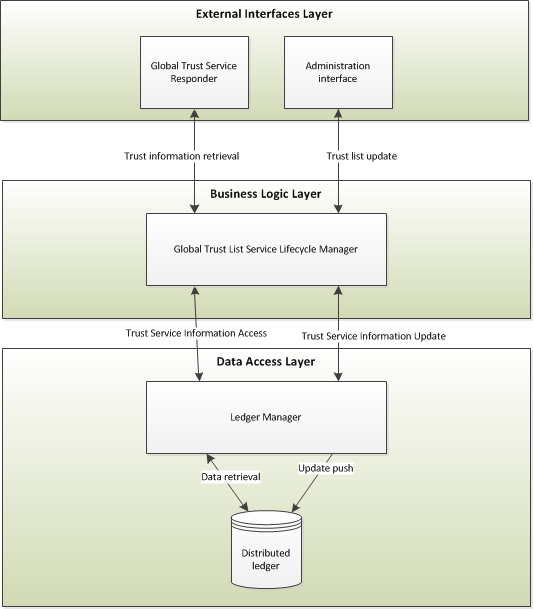
\includegraphics[scale=0.83]{figures/gTSL-3Tier}
	\caption{Architecture 3 tiers de la gTSL. Illustration extraite de \textit{Design documentation}~\cite{design-document}}
	\label{fig:3tier-archi}
\end{figure}

D'un point de vue architectural, la gTSL s'appuie sur une architecture à trois couches:
\begin{itemize}
	\item la couche de services externes qui expose les interfaces externes du système, i.e. le \textit{Global Trust Service Responder} et l'interface d'administration;
	\item la couche métier qui est composée du \textit{Global Trust List Service Lifecycle Manager};
	\item la couche de données qui correspond aux interfaces et aux composants qui permettent de connecter la gTSL à une solution de stockage de données.
\end{itemize}


\subsubsection{Caractéristiques des utilisateurs}

Deux types différents d'utilisateurs ont été identifiés concernant la gTSL:
\begin{itemize}
	\item les utilisateurs d'administration, i.e. les administrateurs des listes, qui peuvent agir au nom d'un État membre de l'UE et qui sont chargés de la maintenance quotidienne et de la gestion des listes de confiance;
	\item les utilisateurs externes, i.e. les personnes et les applications externes qui souhaitent obtenir des informations concernant les statuts de confiance pour un TSP, un TS ou un État membre donné.
	\newline
\end{itemize}

Ces utilisateurs ont accès au système à travers des interfaces dédiées:
\begin{itemize}
	\item les utilisateurs d'administration ont accès à une plateforme de gestion de la gTSL, qui expose sans ambiguïté les différentes fonctionnalités d'administration auxquelles ces utilisateurs doivent avoir accès;
	\item les utilisateurs externes ont accès à la fois à une interface graphique et à une seconde interface de web services\footnote{Un web service correspond à l'implémentation d'une ressource identifiée par une URL.}, qui permet la récupération d'informations concernant les statuts des services de confiance sur base de certificats électroniques fournis par l'utilisateur ainsi que des informations générales concernant les TSPs.
\end{itemize}

\subsubsection{Besoins fonctionnelles}

La gTSL doit supporter l'internationalisation (non-UE) prévue dans le règlement eIDAS. À ce titre, la gTSL doit permettre l'ajout de TSPs déclarés dans un pays qui n'est pas membre de l'UE, qu'ils soient qualifiés ou non.

\subsubsection{Besoins d'utilisation}

La gTSL doit offrir une interface permettant la récupération ainsi que la publication d'informations relatives aux TSPs. L'objectif minimum à remplir pour assurer la conformité avec le standard ETSI TS 119 612~\cite{ETSITS119612} est que la gTSL soit disponible via le protocole HTTP.

\subsubsection{Besoins de performance}

La gTSL doit apporter un stockage interne efficace pour stocker les informations concernant les TSPs et doit être hautement évolutif afin de gérer efficacement de nombreuses quantités de demandes parallèles.

\subsubsection{Interfaces du système}

La gTSL doit exposer, grâce à une interface de web services, les fonctionnalités permettant la récupération d'informations concernant les statuts des services de confiance.

\subsubsection{Interfaces utilisateur}

Les fonctionnalités de gestion de la gTSL doivent être fournies à travers une interface web cohérente et intuitive, permettant aux utilisateurs de l'utiliser sans ambiguïté. 
Les interfaces utilisateur doivent rester cohérentes avec les interfaces utilisateur de l'application actuelle tout en ne montrant aucune ambiguïté en termes de hiérarchie visuelle et de contenu.

\subsubsection{Fiabilité du système}

Le système doit être disponible sur une base de 24 heures par jour et 7 jours par semaine. Plus
particulièrement, le standard ETSI TS 119 612~\cite{ETSITS119612} impose que la récupération des informations concernant les listes de confiance soit disponible sur une base de 24 heures par jour et 7 jours par semaine, avec une disponibilité annuelle minimum de 99.9\%.

\subsubsection{Sécurité du système}

En raison de la nature sensible des données gérées par la gTSL, et de la haute disponibilité requise, les besoins en terme de sécurité doivent garantir que ces données ne peuvent être et ne sont pas compromises. De plus, il est primordial que la gestion des services de confiance et des fournisseurs de services de confiance soit limitée aux personnes autorisées.
En effet, la gTSL ne doit pas permettre à des personnes non autorisées de créer, modifier ou supprimer des informations relatives aux listes de confiance et doit assurer l'intégrité des données qu'elle traite.

\subsection{Besoins logiciels}

\subsubsection{Conformité au standard}

La gTSL doit respecter la syntaxe et la sémantique d'une liste de confiance définies dans le standard ETSI TS 119 612~\cite{ETSITS119612}.

\subsubsection{Rétrocompatibilité}

La gTSL doit pouvoir s'intégrer au schéma existant basé sur la LoTL. Cela signifie qu'elle doit être rétrocompatible avec l'ensemble des listes de confiance actuellement référencées dans la LoTL.

\section{Limites de l'architecture actuelle}
\label{sec:limits}

Dans le modèle actuel, chaque modification apportée au contenu d'une liste nationale induit la nécessité de republier l'entièreté de cette liste. De plus, toute modification apportée sur l'URL\footnote{Une URL (acronyme anglais de Uniform Resource Locator) est couramment appelée adresse web.} à laquelle la liste est distribuée ou sur le certificat utilisé pour signer la liste, induit la nécessité de republier à la fois la liste nationale et la liste européenne.

Le caractère centralisé du système actuel de distribution des listes de confiance contient des 
problèmes éventuels qui doivent être résolus dans le cadre de la globalisation des listes de services de confiance:
\begin{itemize}
	\item les listes de confiance des États membres sont uniquement récupérables après inspection préalable de la LoTL, le schéma actuel est donc sujet à un point individuel de défaillance\footnote{Un point individuel de défaillance (single point of failure ou SPOF en anglais) est un point d'un système informatique dont le reste du système est dépendant et dont une panne entraîne l'arrêt complet du système.};
	\item chaque État membre maintient les données relatives à sa liste de confiance, cela signifie que l'arrêt du nœud de distribution d'un État membre rend ses données non consultables;
	\item l'architecture existante est exposée à un problème de résilience puisqu'elle nécessite que tous les nœuds de distribution des États membres soient actifs afin que la liste globale soit considérée complète et donc fiable;
	\item l'intégrité des données peut être compromise, car si les données d'un État membre sont corrompues localement sur son nœud de distribution, alors l'intégrité globale est compromise puisque la confiance accordée peut être brisée par un seul nœud défaillant;
	\item des problèmes de performance et de latence peuvent être rencontrés puisqu'il est nécessaire de télécharger et valider l'ensemble des informations qui sont réparties sur différents points de distribution;
	\item le schéma actuel ne conserve pas l'historique des modifications, c'est-à-dire qu'une nouvelle publication d'une liste remplace totalement la précédente, ce qui ne permet pas de conserver une trace des modifications mises en œuvre entre les versions, ni de revenir à une version antérieure en cas de problème.
	\newline
\end{itemize}

L'objectif de la gTSL est d'effectuer une refonte de l'architecture actuelle qui a montré ses limites en y apportant des technologies innovantes. Pour cela, il est nécessaire d'adopter un modèle décentralisé et distribué qui permet de résoudre les problèmes de résilience et de point individuel de défaillance sus-cités. Par ailleurs, la technologie blockchain apporte des avantages permettant d'assurer l'intégrité des données ainsi que la sécurité du système.

\section{Gestion de projet}

Cette section a pour objectif d'introduire la méthode Agile qui a été utilisée au cours de ce stage, et d'exposer la répartition du travail réalisé, à l'aide d'un diagramme de Gantt.

\subsection{Méthode de gestion de projet}

La méthode Agile a été utilisée au cours de ce projet. 
Plus particulièrement, l'équipe s'est appuyée sur le schéma Scrum, qui permet un cadre de travail itératif et incrémental où les tâches majeures sont décomposées en sous-tâches.
La méthodologie Scrum est basée sur le découpage d'un projet en sprints\footnote{Un sprint est une période sur laquelle sont réalisées des tâches définies.}, qui sont des cycles de livraison très courts.
Un sprint peut s'étendre sur une durée de quelques heures à un mois. 
Dans notre cas, nous avons choisi une durée de deux semaines par sprint, qui est la durée préconisée dans la méthode.
En début de sprint, une estimation de la durée de chaque tâche est effectuée. Ensuite une planification opérationnelle est réalisée.
Un sprint se termine généralement par une démonstration du travail réalisé, suivie d'une rétrospective afin d'analyser le déroulement du sprint achevé dans le but d'améliorer les pratiques de l'équipe. 
Quotidiennement est organisé un Scrum meeting\footnote{Un Scrum meeting est communément appelé mêlée en français.}, réunion courte et énergique, qui permet à l'équipe de discuter de l'avancée du sprint et de lever les points bloquants du projet.
Afin de suivre la progression des objectifs au fur et à mesure de l’avancement du projet, nous avons utilisé l'outil JIRA\footnote{Voir \url{https://fr.atlassian.com/software/jira}}, qui est un système de gestion de projets. Il a servi notamment à définir les différentes tâches du projet et à répartir le travail entre les membres de l’équipe.

\subsubsection{Les avantages majeurs de Scrum}

Scrum apporte des avantages qui sont définis comme étant les trois piliers de la méthodologie:
\begin{itemize}
	\item la transparence, par l'utilisation d'un langage commun afin de permettre à tout un chacun d'obtenir rapidement une bonne compréhension du projet; 
	\item l'inspection, par l'analyse quotidienne du travail accompli et restant lors des sprints, afin de repérer tout indicateur indésirable;
	\item l'adaptation, dans le cas d'une dérive après inspection, des ajustements doivent être effectués afin de minimiser les écarts de réalisation.
\end{itemize}

\subsection{Organisation du temps}

La Figure~\ref{fig:gantt} présente un diagramme de Gantt qui expose de manière globale la répartition du travail réalisé. Ce diagramme est volontairement non détaillé puisque l'utilisation de la méthodologie Agile ne permet pas d'organiser à l'avance et avec précision la réalisation des tâches. Il est important de noter que le diagramme se termine à la date de fin du stage mais que la livraison du projet est prévue au 30 novembre 2017.

\begin{figure}[h]
	\centering
	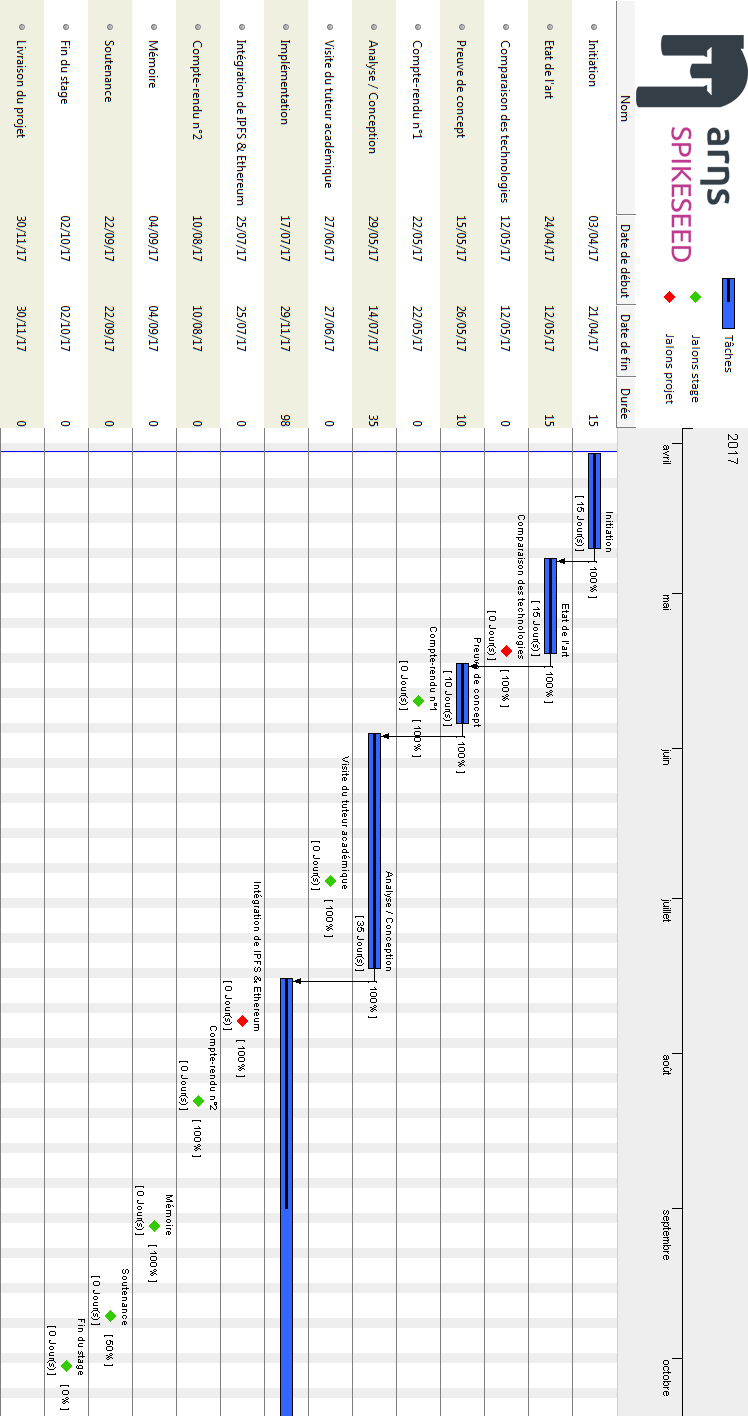
\includegraphics[scale=0.67]{figures/gantt-stage-vertical}
	\caption{Diagramme de Gantt}
	\label{fig:gantt}
\end{figure}

\clearpage

Le diagramme de Gantt en Figure~\ref{fig:gantt} permet d'avoir un aperçu de l'organisation du stage. Le stage s'est déroulé sur une période de six mois, du 3 avril 2017 au 30 septembre 2017. Durant cette période, j'ai été amené à réaliser différentes tâches qui sont détaillées dans la suite de ce mémoire. D'un point de vue générale, le stage a été décomposé en cinq parties majeures qui sont décrites ci-après.

\subsubsection{Initiation}

La phase d'initiation a commencé dès le début du stage et a duré environ trois semaines. 
Elle peut être décomposée en deux sous-parties. Dans un premier temps, j'ai dû me familiariser avec le projet. Pour réaliser cela, j'ai eu accès au document de conception de la gTSL~\cite{design-document} qui explique, d'une manière générale et sans précision de technologies, l'architecture à mettre en place ainsi que les cas d'utilisation à implémenter dans le cadre du projet FutureTrust. J'ai pris connaissance du standard ETSI TS 119 612~\cite{ETSITS119612} qui détaille le format à respecter dans le cadre des listes de confiance. Dans un second temps, j'ai effectué des recherches sur les notions de cryptographie, de signature électronique et de blockchain afin de les mettre en œuvre dans le projet. Cette seconde partie a été la préparation du travail suivant qui est l'état de l'art.

\subsubsection{État de l'art}

La seconde phase, ayant pour objectif d'établir un état de l'art, a suivi la phase d'initiation et s'est étendue sur trois semaines.
L'état de l'art est un processus qui vise à explorer l'état des connaissances et technologies actuelles dans un domaine spécifique. Pour notre projet, l'état de l'art a porté sur la blockchain ainsi que les systèmes  décentralisés. Le but de cette phase a été d'explorer le plus largement possible les technologies pouvant être utilisées dans le projet afin de les comparer pour choisir par la suite la solution la plus adaptée à nos besoins. Cette étape a donné lieu à un livrable qui a été inclus dans le document de conception de la gTSL comme le montre le jalon "Comparaison des technologies" dans la Figure~\ref{fig:gantt}. Ce document est disponible en Annexe~\ref{anx:comparison}. L'état de l'art est détaillé dans le Chapitre~\ref{chap:state-of-the-art}.

\subsubsection{Preuve de concept}

À la suite de l'état de l'art, un choix technologique a été effectué. L'étape suivante a donc consisté à prouver que les choix opérés correspondent aux besoins du projet. Pour cela, j'ai pu réaliser une preuve de concept sur une durée de quinze jours. Cette phase a ensuite donné lieu à une démonstration à l'équipe afin de valider de manière définitive les choix technologiques. Le détail de la preuve de concept ainsi que la justification des choix opérés sont présentés dans le Chapitre~\ref{chap:realisation}.

\subsubsection{Analyse / Conception}

La phase d'analyse et conception a été précédée de la preuve de concept qui a permis de valider les technologies à utiliser pour le projet. Dans le cadre de cette phase, nous avons déterminé les modules à implémenter afin de répondre aux besoins exprimés dans le document de conception. L'analyse et la conception ont consisté à envisager différentes solutions quant à la mise en place d'une architecture décentralisée basée sur une blockchain, en étant conforme aux différentes contraintes définies dans le document de conception et en s'appuyant sur les technologies choisies. Cette partie a duré un mois et demi, et est détaillée dans le Chapitre~\ref{chap:analyse}.

\subsubsection{Implémentation}

La dernière phase, et la plus conséquente, est l'implémentation. Elle consiste à développer la solution conçue et imaginée lors de la phase d'analyse et conception. Lors de la rédaction de ce mémoire, cette phase est en cours de réalisation. Cette phase est découpée en sprints d'une durée de deux semaines. L'implémentation est détaillée dans le Chapitre~\ref{chap:realisation}. 

\chapter{État de l'art}
\label{chap:state-of-the-art}

Dans le cadre du projet FutureTrust, il a été nécessaire d'effectuer un état de l'art afin d'avoir une vue globale de l'état actuel de la technologie blockchain et des technologies distribuées et décentralisées comme les bases de données ou les systèmes de fichiers. Pour cela, il convient de décrire l'émergence de la blockchain ces dix dernières années, d'expliquer les avantages qu'apporte la décentralisation dans les systèmes actuels et d'établir une liste des technologies existantes. L'état de l'art a pour intérêt de soulever l'effervescence autour de ces technologies ainsi que d'opérer les meilleurs choix dans la réalisation du module de gTSL. Les solutions existantes présentées en Section~\ref{sec:solutions} ont été envisagées afin de mettre en place un système permettant de conserver, gérer et récupérer les données de la gTSL de manière sécurisée et apportant une forte résilience.

\section{L'émergence de la blockchain}

Cette section a pour objectif de mettre en avant l'origine de la blockchain en détaillant les recherches antérieures à cette technologie, et d'analyser son état actuel et les améliorations qui peuvent être apportées dans le futur.

\subsection{Historique}

Le concept de monnaie numérique, ainsi que d'autres applications comme les registres de propriété, existent depuis des décennies. 
Les protocoles de paiement apparus dans les années 1980 et 1990, connus sous le nom de e-cash\cite{ecash} et reposant sur des concepts cryptographiques, avaient pour but de fournir une monnaie avec un degré élevé de confidentialité. La mise en place de ces protocoles a largement échoué à cause de leur dépendance à un intermédiaire centralisé. 
En 1998, la technologie B-money\cite{bmoney} créée par Wei Dai voit le jour, et devient la première proposition introduisant l'idée de créer de l'argent en résolvant des puzzles informatiques en se basant sur un consensus décentralisé. Cependant, cette proposition a été peu détaillée sur la manière dont le consensus décentralisé pouvait effectivement être mis en œuvre. 
En 2005, Hal Finney a introduit le concept de preuves de travail réutilisables, un système basé sur des idées de b-money en les combinant aux puzzles Hashcash\cite{hashcash} difficiles à calculer créés par Adam Back, afin de créer un concept de crypto-monnaie. Mais encore une fois, cette proposition n'a pas su être exploitée. 
En 2009, une monnaie décentralisée a été pour la première fois mise en œuvre par Satoshi Nakamoto, combinant les différentes propositions établies pour la gestion de la propriété par l'utilisation de clés publiques avec un algorithme de consensus permettant de suivre l'identité du possesseur de la monnaie, appelé preuve de travail (Proof of Work). C'est la naissance du Bitcoin et plus généralement de la blockchain.

Le mécanisme derrière la preuve de travail a été une avancée car il résout simultanément deux problèmes. 
Tout d'abord, il fournit un algorithme de consensus simple et modérément efficace, permettant aux nœuds du réseau de convenir collectivement d'un ensemble de mises à jour du registre Bitcoin. 
Ensuite, il fournit un mécanisme qui permet l'entrée libre d'un nouveau membre dans le processus de consensus, ce qui résout le problème engendré par l'influence d'un membre dans le consensus, tout en empêchant les attaques Sybil\footnote{Une attaque Sybil est une attaque informatique qui vise à renverser un système par la création de fausses identités dans un réseau pair-à-pair.}. 
Dans la preuve de travail, le poids d'un nœud dans le processus de vote par consensus est directement proportionnel aux ressources de calcul que ce nœud apporte. 
Depuis cela, une approche alternative, appelée preuve d'enjeu (Proof of Stake), initiée par Peercoin\cite{peercoin} a été proposée, dans laquelle le poids d'un nœud est proportionnel à la quantité de crypto-monnaie qu'il détient et non plus aux ressources informatiques qu'il apporte.

\subsection{État actuel et potentiel futur}

Actuellement deux principaux protocoles publics se sont démarqués. Le premier est bien entendu Bitcoin et le second est le récemment créé Ethereum. 
Malgré les solutions qu'ils apportent, les défis et les développements potentiels de la blockchain restent nombreux.
Premièrement, c'est une technologie très récente, complexe et évoluant rapidement, de laquelle une effervescence a été créée depuis quelques années mais qui souffre encore de problèmes de maturité.
Bien que l'implémentation de Bitcoin soit stabilisée, ce n'est pas le cas pour les technologies émergentes comme Ethereum.

Le travail à effectuer pour permettre à la technologie de se stabiliser et de se populariser reste colossal:
\begin{itemize}
	\item le développement d'outils à destination du grand public permettant d'interagir facilement avec la blockchain;
	\item l'amélioration des protocoles de consensus (preuve de travail, preuve d'enjeu, etc.);
	\item l'augmentation du nombre de transactions traitées par seconde;
	\item la création et l'amélioration d'outils pour le développement d'applications basées sur l'utilisation de la blockchain;
	\item la recherche sur les bonnes pratiques pour la sécurité des contrats intelligents;
	\item la mise en place de protocoles de désidentification pour les transactions.
	\newline
\end{itemize}
Cette liste n'est pas exhaustive et les tâches à accomplir sont énormes.
Malgré tout, les personnes impliquées sur les différents projets de blockchain sont désireux de faire avancer cette technologie et la recherche progresse rapidement.

Comme conséquence naturelle de sa nouveauté, la technologie est également mal comprise.
Il est possible d'avoir lu de nombreux articles sur le sujet sans en avoir réellement compris le fonctionnement ou l'intérêt.
En effet, il existe énormément d'informations sur la blockchain et notamment sur les possibilités de son utilisation mais peu d'articles expliquent clairement et de manière détaillée son fonctionnement.
La nouveauté de la technologie explique également celle de son écosystème, ce n'est qu'en 2013 que les premières plate-formes d'échange de crypto-monnaie sont apparues.
À l'heure actuelle, le secteur est en plein essor, et de nombreuses start-ups ainsi que des initiatives de grandes entreprises ont été lancées.
Dans cet environnement, il existe encore un élément totalement manquant qui est la gestion de l'identité.
Sur une blockchain publique, tout le monde est anonyme. En effet, un utilisateur est uniquement identifié par une clé publique et non par son identité.
L'anonymat est un avantage dans certains types d'utilisation, mais d'autres utilisations nécessitent une identité qui peut être certifiée et associée à un compte en particulier. Il est donc nécessaire que ce compte puisse être récupéré par son propriétaire légitime en cas de perte.
Il s'agit d'une question complexe majeure découlant de la conception de la technologie. Cependant, de nombreuses initiatives sont en cours dans ce domaine comme par exemple uPort\footnote{Voir \url{https://www.uport.me/}, uPort est un système d'identité entièrement autonome basé sur Ethereum.} de ConsenSys\footnote{Voir \url{https://consensys.net/}, ConsenSys est une entreprise développant des applications décentralisées et des outils pour le développement d'applications basées sur l'utilisation de la blockchain.}.
Depuis la création d'Ethereum, cet écosystème comprend également des entités émergentes sur la blockchain, à savoir les applications décentralisées, plus communément appelées dApp\footnote{acronyme anglais de decentralized application.}.
La sécurité des smart contracts est encore à un stade précoce, et des efforts considérables seront nécessaires avant d'envisager l'automatisation des opérations à très forte valeur ajoutée.
De nombreuses initiatives ont déjà été lancées à cet égard et se poursuivront comme la recherche fondamentale, les logiciels d'analyse formelle, l'amélioration du langage ou encore de la machine virtuelle Ethereum.
De nombreux projets dApp ont été financés cette année, en particulier par le biais de l'ICO\footnote{
ICO (acronyme anglais de Initial Coin Offering) est le processus par lequel une entité innovante offre aux investisseurs certaines quantités d'une nouvelle crypto-monnaie ou crypto-token en échange d'une quantité de crypto-monnaie existante comme Bitcoin ou Ethereum.}.

De nombreux types d'utilisation de la blockchain sont donc en cours de développement.
Ces utilisations ont besoin d'avoir des règles détaillées et un cadre juridique défini. Malheureusement, dans l'état actuel des choses, la loi n'encadre pas la technologie aussi bien au niveau de la reconnaissance juridique des nouveautés apportées qu'au niveau des restrictions ou des contrôles de son utilisation.
La reconnaissance de ces caractéristiques par le droit local, le droit européen et les traités internationaux serait une avancée majeure dans de nombreux secteurs comme la finance, la santé ou l'énergie, et permettrait aux entreprises de créer des systèmes innovants.
Ce manque de reconnaissance officielle a également une incidence sur la participation du secteur privé.
Si l'Europe veut être un précurseur de la révolution blockchain, elle doit s'impliquer davantage, tant au niveau national qu'international.

Dans le futur, il sera important de s'intéresser aux point suivants:
\begin{itemize}
	\item les développements techniques majeurs tels que la vérification formelle des contrats intelligents, la preuve d'enjeu ou la gestion de l'identité;
	\item la reconnaissance par le secteur public et privé des crypto-monnaies et plus généralement des enregistrements dans la blockchain;
	\item les projets en cours de développement qui seront lancés à court et à moyen terme comme les projets impliquant des blockchains et des dApps.
\end{itemize}

\section{La décentralisation du Web}

Le but initial du web et de l'Internet était de créer un réseau neutre commun auquel chacun puisse participer de manière égale afin d'améliorer l'humanité. Heureusement, il existe un mouvement émergent pour ramener le web à cette vision et implique même certains des éléments clés de la naissance du web. C'est ce qu'on appelle le Web décentralisé ou le Web 3.0. Il décrit une tendance émergente pour la création de services sur Internet qui ne dépendent pas d'une seule organisation centrale.
La participation égale sur Internet s'est rapidement effondrée lorsque des personnes se sont rendues compte qu'un moyen simple de créer de la valeur sur ce réseau était de construire des services centralisés qui rassemblent, piègent et monétisent des informations.
Les moteurs de recherche comme Google, les réseaux sociaux comme Facebook, les applications de discussion comme WhatsApp se sont imposés en fournissant des services centralisés sur Internet.

Dans le même temps, ces organisations réduisent les libertés fondamentales de l'Internet telles que la possibilité de lier du contenu via une URL ou la possibilité pour les moteurs de recherche d'indexer son contenu.
Le Web décentralisé envisage un monde futur où des services tels que la communication, la monnaie, l'édition, les réseaux sociaux ou la recherche sont fournis non pas par des services centralisés appartenant à des organisations individuelles, mais par des technologies alimentées par la communauté des utilisateurs.
L'idée principale de la décentralisation est que l'exploitation d'un service n'est pas confiée à une seule entreprise omnipotente. Au lieu de cela, la responsabilité du service est partagée soit par une exécution sur plusieurs serveurs fédérés, ou par l'exécution d'applications côté client s'appuyant sur un modèle distribué.
Les règles qui décrivent le comportement d'un service décentralisé sont conçues pour obliger les participants à agir de manière équitable, grâce à l'utilisation de techniques cryptographiques telles que les arbres de Merkle\footnote{Un arbre de Merkle, aussi appelé arbre de hachage, est une structure de données contenant l'empreinte d'un volume de données.} et la signature électronique pour favoriser la responsabilité des participants.

Il existe trois concepts fondamentaux que le Web décentralisé prône:
\begin{itemize}
	\item la confidentialité, en effet la décentralisation impose une attention accrue à la confidentialité des données. Les données sont réparties sur le réseau et les technologies de chiffrement sont essentielles pour garantir que seuls les utilisateurs autorisés puissent modifier les données qui leur appartiennent. L'accès aux données est entièrement contrôlé par le réseau grâce à des algorithmes. Ce modèle montre une césure avec les réseaux centralisés où le propriétaire du réseau a un accès complet aux données, et donc facilite l'établissement du profil du client et le ciblage publicitaire;
	\item la portabilité des données, dans un environnement décentralisé, les utilisateurs possèdent leurs données et choisissent avec qui ils partagent ces données. En outre, ils en conservent le contrôle et ils peuvent les transférer d'un service à un autre librement.
	\item la sécurité, les environnements décentralisés sont plus sûrs contre le piratage, l'infiltration, l'acquisition et les pannes que les environnements centralisés, car ils ont été construits pour être exposés publiquement dès le départ.
	\newline
\end{itemize}

De nombreux services auparavant centralisés et aujourd'hui remplacés par des services décentralisés ont montré que cette approche peut être mise en œuvre et qu'une alternative du web existant entièrement décentralisée est réalisable. 
Parmi les systèmes décentralisés qui ont connu un grand succès on peut par exemple citer Git, un système de gestion de versions entièrement décentralisé, remplaçant presque totalement des systèmes centralisés comme par exemple Subversion. 
Au même titre, Bitcoin a démontré qu'une monnaie peut exister sans autorité centrale, en contraste avec un service centralisé tel que Paypal. 
Diaspora vise quant à lui à fournir une alternative décentralisée à Facebook.
Cependant, la plupart de ces technologies ont toujours été laissées de côté par le grand public. Mais aujourd'hui, les utilisateurs se rendent compte que la dépendance aux plates-formes communautaires massives qui contrôlent Internet n'est pas dans leurs intérêts.

Il existe déjà une nouvelle génération de systèmes décentralisés qui ont attiré l'attention de l'industrie traditionnelle.
Blockstack\footnote{Voir \url{https://blockstack.org/}, Blockstack est la première implémentation de système décentralisé de noms de domaine s'exécutant sur la blockchain Bitcoin.} et Ethereum montrent que la blockchain peut être plus qu'une simple crypto-monnaie. IPFS et le projet Dat\footnote{Voir \url{https://datproject.org/}, Dat est un outil de partage de données distribuées.} fournissent également des gestionnaires décentralisés de données, où la propriété et la responsabilité des données sont partagées par tous ceux qui y accèdent, ne reposant plus sur un hébergement centralisé.

Bien que le Web décentralisé attire l'intérêt et la passion de la communauté des développeurs, il est actuellement impossible de dire quelles nouvelles économies émergeront et quelles sortes de nouvelles technologies et services vont être inventés. La seule certitude que nous ayons est que la décentralisation du Web est une réalité et que les personnes actives autour de cette révolution soutiendront les intérêts de leurs utilisateurs.

\section{Solutions existantes}
\label{sec:solutions}

La couche de persistance des données de la gTSL repose sur la blockchain et des concepts de décentralisation. À ce titre, l'objectif est de conserver toutes les informations relatives aux TSPs et aux TSs dans un registre sécurisé et de répliquer toutes les données de la gTSL à travers un réseau pair-à-pair\footnote{Le pair-à-pair est un modèle de réseau informatique similaire au modèle client-serveur mais où chaque client est aussi un serveur.} décentralisé.
Cela permet de garantir l'intégrité et la disponibilité des informations, puisque chaque donnée est signée et est accompagnée de toutes les données qui la précèdent dans le registre. La distribution de l'information à travers un réseau pair-à-pair fournit une résilience forte contre les attaques par déni de service.

Afin d'atteindre cet objectif qui permettra de pallier aux problèmes de l'architecture actuelle, plusieurs options ont été envisagées :
\begin{itemize}
	\item stocker les données dans une blockchain publique existante;
	\item stocker les données dans une blockchain privée;
	\item stocker les données dans une blockchain privée, et utiliser une blockchain publique pour s'assurer de l'intégrité des données (par exemple en conservant le hash\footnote{Un hash est le résultat d'une fonction de hachage qui permet d'identifier rapidement une donnée.} de la transaction réalisée sur la blockchain privée dans une blockchain publique);
	\item stocker les données dans un système décentralisé et distribué, comme par exemple une base de données ou un système de fichiers, et utiliser une blockchain publique pour s'assurer de l'intégrité des données (par exemple en conservant le hash des données).
	\newline
\end{itemize}

Cette section présente les technologies qui ont été envisagées en tant que solutions de stockage de données dans le cadre de l'implémentation de la gTSL. On y retrouve des technologies de blockchain, mais aussi des systèmes décentralisés et distribués.

\subsection{Ripple}

Ripple\footnote{Voir \url{https://ripple.com/}} est une crypto-monnaie s'appuyant sur un registre distribué basé sur une blockchain qui n'utilise pas de système de preuve de travail pour l'ajout de blocs. Au lieu de cela, il repose sur un mécanisme de consensus (The Ripple Protocol Consensus Algorithm, 2014) appliqué à un sous-réseau de nœuds connus et fiables. Cette technologie est surtout orientée vers les paiements, les transactions et les échanges de crypto-monnaie mais ne propose pas de réelle solution pour le stockage des données.

\subsection{Tendermint}

Tendermint\footnote{Voir \url{https://tendermint.com/}} est une crypto-monnaie s'appuyant sur un registre distribué basé sur une blockchain qui utilise un système de votes par un consensus au lieu du minage. À ce titre, Il repose sur un ensemble de nœuds de validation dont la responsabilité est d'émettre des votes signés pour ou contre l'ajout de nouveaux blocs dans la chaîne. Le scrutin est validé si au minimum les deux tiers des nœuds de validation votent pour l'acceptation d'un nouveau bloc. Tendermint apporte uniquement une solution concernant l'utilisation d'un système de votes à la place d'une preuve de travail.

\subsection{Ethereum}
\label{sec:ethereum}

Ethereum\footnote{Voir \url{https://ethereum.org/}} est une plate-forme publique décentralisée et distribuée basée sur la technologie blockchain. Elle repose sur des programmes dont le code et les données sont stockés sur la blockchain. Ces programmes s'appellent des smart contracts. 
Ethereum apporte donc l'utilisation de concepts de blockchain au-delà du cas d'utilisation de la crypto-monnaie et offre un environnement virtuel d'exécution qui peut être utilisé pour créer des organisations autonomes décentralisées, i.e. des organisations qui sont gérées par des règles spécifiées dans des smart contracts. Ethereum étant conçu principalement comme un environnement d'exécution décentralisé et autonome, il n'offre pas de réelles fonctionnalités de stockage. Bien que les données puissent être stockées dans le cadre de l'exécution des contrats intelligents, le coût de son utilisation peut rapidement devenir prohibitif. En effet, le système est conçu pour calculer le coût des transactions en fonction des ressources nécessaires en termes de calcul, de bande passante et de stockage.

\subsection{Swarm}

Swarm\footnote{Voir \url{http://swarm-gateways.net/bzz:/swarm-gateways.eth/}} est une plate-forme de stockage distribuée ainsi qu'un service de distribution de contenu directement lié à Ethereum. Son objectif initial est de servir de solution de stockage décentralisé et redondant pour les enregistrements dans le registre public d'Ethereum, mais il peut également être utilisé comme solution de stockage à part entière et de service pair-à-pair. Au moment de la rédaction de ce mémoire, Swarm était encore à ses débuts de développement, avec uniquement une version "alpha" disponible.

\subsection{Hyperledger Fabric}

Hyperledger Fabric\footnote{Voir \url{https://www.hyperledger.org/projects/fabric}} est une plate-forme reposant sur un registre distribué destinée à l'exécution de smart contracts. Il est conçu selon une architecture modulaire, prend en charge les contrats intelligents écrits dans le langage de programmation Go et repose sur un réseau de pairs de validation (c'est-à-dire les nœuds responsables du maintien du registre) et de pairs de non validation. À l'instar d'Ethereum, Hyperledger ne gère pas le stockage de données nativement et simplement, mais son architecture modulaire pourrait le permettre.

\subsection{Keyless ledger}

Keyless Signature Infrastructure\footnote{Voir \url{https://guardtime.com/technology/ksi-technology}} (KSI) est une plate-forme offrant une authentification basée sur la signature électronique pour les données numériques, les machines et les humains. KSI repose uniquement sur les fonctions de hachage, son registre agit comme un enregistrement de timestamps\footnote{Le timestamping, aussi nommé horodatage en français, est un mécanisme qui consiste à associer une date et une heure à un événement, une information ou une donnée informatique.} émis pour les hashes de données soumises par les utilisateurs. Son intérêt est de fournir des signatures électroniques, et selon les dires des développeurs d'une manière plus sécurisée que la Public Key Infrastructure\footnote{La PKI est une infrastructure visant à fournir une garantie de confiance dans la validité d’une identité numérique et utilisant pour cela une pair de clé liée à un certificat.} (PKI).

\subsection{OpenChain}

OpenChain\footnote{Voir \url{https://www.openchain.org/}} est un registre distribué open-source qui repose uniquement sur une signature électronique qui est générée pour les transactions qu'il enregistre. Les transactions sont directement liées les unes aux autres, sans l'utilisation de blocs, et peuvent maintenir des données. OpenChain peut posséder plusieurs instances, chacune répliquant les autres. Cependant, la technologie est construite autour d'une hiérarchie de nœuds de validation et de nœuds d'observation. Les nœuds de validation peuvent ajouter et valider des transactions pour le registre. Les nœuds d'observation peuvent uniquement répliquer les données des nœuds de validation auxquels ils sont connectés. Par conséquent, il n'est pas possible d'implémenter un réseau purement décentralisé d'instances OpenChain.

\subsection{BigchainDB}

BigchainDB\footnote{Voir \url{https://www.bigchaindb.com/}} vise à interfacer la technologie blockchain et une base de données en ajoutant des caractéristiques de la blockchain comme la décentralisation, l'immutabilité et l'échange d'actifs à une implémentation d'une base de données NoSQL\footnote{NoSQL, pour Not only SQL, est une famille de systèmes de gestion de base de données (SGBD) qui s'écarte du paradigme classique des bases relationnelles.} existante. Cette technologie en est encore à ses débuts de développement et manque actuellement de contrôles de sécurité de base (par exemple, un administrateur de base de données supprimant une base de données sur un nœud verra cette opération être répliquée sur tous les autres nœuds). De plus, BigChainDB n'est pas Byzantine Fault Tolerant\footnote{	La Byzantine fault tolerance (BFT) est la caractéristique d'un système qui tolère la classe de défaillances connue sous le nom du problème des généraux byzantins pour lesquels il existe une preuve de non-solvabilité} (BFT).

\subsection{InterPlanetary File System (IPFS)}

IPFS \footnote{Voir \url{https://ipfs.io/}} est un système de fichiers distribué pair-à-pair qui cherche à connecter tous les périphériques informatiques avec un même système de fichiers. Il réutilise le paradigme de la blockchain, plus précisément les concepts d'immutabilité des données et de la décentralisation réalisée à travers une communication pair-à-pair, tout en s'inspirant du système de contrôle de version Git\footnote{Voir \url{https://ripple.com/}}. Il permet notamment de stocker des informations, de tous types et de tous volumes, qui sont répliquées à travers le réseau. 

\subsection{Monax}

Monax\footnote{Voir \url{https://monax.io/}} est une plate-forme open-source qui vise les développeurs qui veulent construire et exécuter des applications basées sur la blockchain pour des écosystèmes business. Il peut être comparé à Ethereum, toutefois avec des autorisations qui le rendent juridiquement utilisable dans les environnements commerciaux. Cette technologie a pour intérêt de mettre en place sa propre plate-forme de blockchain dans un environnement business.

\subsection{Factom}

Factom\footnote{Voir \url{https://www.factom.com/}} fournit un protocole distribué et décentralisé qui s'exécute sur la blockchain Bitcoin, et qui maintient un registre inaltérable. Cette technologie a pour but de conserver les documents des entreprises de manière sécurisée.

\subsection{Emercoin}

Emercoin\footnote{Voir \url{https://emercoin.com/}} est une crypto-monnaie utilisant un minage qui repose sur la preuve de travail et la preuve d'enjeu\footnote{en anglais, Proof of Stake.}. Il diverge des crypto-monnaies "standard" dans le sens où sa blockchain ne se limite pas à une utilisation de registre de transactions. Hormis l'utilisation de la crypto-monnaie, d'autres services sont supportés comme un système décentralisé de noms de domaine ou un stockage sécurisé pour des timestamps. Malgré tout, il n'est pas conçu pour le stockage de données.

\section{Synthèse}

Nous avons effectué les choix technologiques inhérents à l'architecture de notre système après une analyse de la technologie blockchain, et suite à une prise en considération de ses avantages et inconvénients.

\subsection{Avantages de la blockchain}

Si cette technologie connaît un tel succès c'est parce qu'elle apporte de nombreux avantages : 
\begin{itemize}
	\item la décentralisation, qui signifie que son architecture ne repose pas sur une entité centrale et permet d'enregistrer des données dans un réseau distribué; 
	\item la transparence, puisque l'état des données conservées est consultable publiquement par tout le monde; 
	\item l'autonomie, puisqu'elle est basée sur un consensus dans lequel chaque partie prenante peut transférer des données de manière sécurisée et autonome;
	\item l'immutabilité, en effet toute transaction est persistée définitivement et donc ne peut être effacée;
	\item l'anonymat, car tout utilisateur de la blockchain est anonyme dans le sens où il n'est pas désigné par son identité mais uniquement par une clé publique\footnote{Une clé publique est un encodage rendu public dans le cadre d'un échange d'informations utilisant le principe de la cryptographie asymétrique.}.
\end{itemize}

\subsection{Inconvénients de la blockchain}
\label{sec:drawbacks-blockchain}

Bien que la blockchain apporte de nombreux avantages, elle comporte aussi des inconvénients :
\begin{itemize}
	\item la performance, en effet cette technologie est et sera toujours plus lente qu'une base de données centralisée puisqu'elle nécessite pour chaque transaction une vérification de signature, une validation par le consensus et la redondance des informations; 
	\item la consommation énergétique, puisque la validation de blocs repose sur la résolution d'un puzzle cryptographique nécessitant une grande puissance de calcul; 
	\item le coût, dans le cas où il est nécessaire d'effectuer un grand nombre de transactions coûteuses;
	\item la confidentialité, puisque toute information enregistrée dans la blockchain est publique, il est fortement déconseillé d'y stocker des informations confidentielles ou personnelles, même si elles sont chiffrées.
\end{itemize}

\subsubsection{Le problème du coût des transactions d'une blockchain dans le cadre du stockage de données}

Toutes les technologies énoncées ci-dessus ont été envisagées dans le cadre du stockage des données liées à la gTSL. Toutes les données doivent être stockées dans un réseau décentralisé et distribué, et doivent être publiques. L'inconvénient majeur des technologies de blockchain est le coût, en matière de crypto-monnaie, du stockage d'un grand volume de données. En effet, comme énoncé en Section~\ref{sec:ethereum}, la preuve de travail qui permet de sécuriser la création de nouveaux blocs dans la blockchain a été conçue pour calculer le coût des transactions en fonction des ressources nécessaires en termes de calcul, de bande passante et de stockage. Si l'on prend l'exemple de la blockchain Ethereum, en se basant sur le prix de l'ether\footnote{L'ether (ETH) est la crypto-monnaie utilisée sur la blockchain Ethereum.} (ETH) qui est d'environ 250€ au moment de la rédaction de ce mémoire, le stockage de 1Go de données coûterait 640 000€.

\subsection{Le choix opéré}
\label{sec:choice}

Dans cette section sont détaillées les différentes solutions préconisées, présentées en Section~\ref{sec:solutions}, dans le cadre du stockage des données de la gTSL. Pour chacune d'entre elles sont exposés ses avantages et ses inconvénients.
Le choix opéré a été validé par la réalisation d'une preuve de concept présentée en Section~\ref{sec:realisation-ledger}.

\subsubsection{Stockage dans une blockchain publique}

La première solution de stocker les données directement dans une blockchain publique existante a l'avantage d'être relativement simple à mettre en place. En effet, cette solution nécessite uniquement de connecter le système au réseau de la blockchain et de soumettre des transactions contenant les données. Malgré cela, la technologie blockchain ne vise pas à stocker des grands volumes de données, ce qui explique le coût de stockage élevé qui rend son utilisation en tant que base de données inefficace.

\subsubsection{Stockage dans une blockchain privée}

La seconde solution de stocker les données dans une blockchain privée a l'avantage d'être relativement peu coûteuse puisque la blockchain est fermée à un nombre restreint de nœuds connus qui ont à charge d'en maintenir l'état. L'inconvénient est que le consensus d'une blockchain privée est faible ce qui le rend vulnérable aux attaques Sybil. En effet, le nombre de nœuds honnêtes est relativement faible ce qui engage la sécurité et l'intégrité des données. Si l'on prend l'exemple d'une blockchain privée maintenue par dix nœuds considérés honnêtes où leur poids de vote est d'une valeur égale à 1, alors un attaquant qui arriverait à connecter onze autres nœuds à cette blockchain (en considérant que ces nœuds ont aussi un poids de vote égal à 1) deviendra majoritaire et pourra corrompre les données de la blockchain puisqu'il a brisé le consensus. Cela est beaucoup plus difficile à produire dans une blockchain publique comme Ethereum car le nombre de nœuds honnêtes est très important.

\subsubsection{Stockage dans une blockchain privée, et utilisation d'une blockchain publique pour assurer l'intégrité des données}

Une autre solution envisagée est de stocker les données dans une blockchain privée, et d'utiliser une blockchain publique pour s'assurer de l'intégrité des données, mais cela complexifie l'architecture par l'utilisation de deux blockchains. De plus, comme dit précédemment, une blockchain n'est pas conçue pour être utilisée en tant que base de données, car un des inconvénients est la performance. En effet, cette technologie sera toujours plus lente qu'une base de données puisqu'elle nécessite pour chaque transaction une vérification de signature et une validation par le consensus. 

\subsubsection{Stockage dans un système décentralisé et distribué, et utilisation d'une blockchain publique pour assurer l'intégrité des données}

La dernière solution de stocker les données dans un système de fichiers décentralisé et distribué et d'utiliser une blockchain publique afin de s'assurer de l'intégrité des données est la solution la plus pertinente dans le cadre de la mise en place de la gTSL. 
IPFS a été choisi en tant que système de fichiers, cette technologie a l'avantage d'être "content-addressable", c'est-à-dire que l'on peut récupérer les données grâce à l'utilisation d'un hash.
Ethereum a été choisi en tant que blockchain, elle a pour rôle de conserver le hash des données.
L'avantage d'un système de fichiers décentralisé et distribué est qu'il permet de stocker des grands volumes de données qui seront automatiquement répliqués à travers les nœuds du réseau. Cela apporte une forte résilience contre les attaques par déni de service et évite un point individuel de défaillance.
L'avantage de la blockchain est qu'elle permet la transparence des données dans un réseau public, qu'elle assure l'intégrité et l'immutabilité des données grâce à un consensus et qu'elle fournit un anonymat aux utilisateurs.
Ce système permet donc de réduire les coûts puisque l'on stocke uniquement un hash servant à identifier les données dans la blockchain. Ce hash a une taille de quelques octets seulement.
Malgré cela, l'architecture est complexifiée puisque l'on interface deux technologies distribuées et il est donc nécessaire de déployer à la fois un nœud IPFS et un nœud Ethereum.

\chapter{Analyse du problème et solution élaborée}
\label{chap:analyse}

Le système de gTSL a été réalisé dans le cadre du projet FutureTrust qui a pour objectif de faciliter l'utilisation de l'identification et de la signature électronique, et qui vise plus particulièrement à mettre en application le règlement de l'UE sur l'identification électronique et les services de confiance pour les transactions électroniques sécurisées au sein de l'UE.
La solution élaborée consiste à étendre l'infrastructure existante de la liste européenne de services de confiance. L'objectif est de mettre en place un système utilisant une architecture décentralisée basée sur la blockchain afin de conserver et de distribuer les informations relatives aux listes de confiance, nommées Trust Service List (TSL). Dans ce chapitre est détaillée l'analyse du système à implémenter afin de répondre aux besoins énoncés dans la Section~\ref{sec:description} et de pallier aux problèmes de l'architecture actuelle énoncés dans la Section~\ref{sec:limits}. 

Dans ce chapitre, nous détaillons les technologies résultantes du choix opéré présenté en Section~\ref{sec:choice}. Ensuite, nous exposons les différents acteurs du système ainsi que leurs rôles. Puis, nous présentons les cas d'utilisation de la gTSL. Enfin, les modules du système, les processus métier ainsi que le modèle de données sont développés.

\section{Description détaillée des technologies utilisées}

Cette section a pour objectif d'apporter des précisions sur l'utilisation des technologies IPFS et Ethereum afin de comprendre leur fonctionnement.

\subsection{Ethereum}

Ethereum~\cite{eth} est une plate-forme de blockchain open-source qui permet à qui le souhaite de créer et d'utiliser des applications décentralisées qui s'exécutent sur la blockchain. 
La particularité de la blockchain Ethereum est qu'elle a été conçue pour permettre aux utilisateurs d'écrire et d'exécuter des smart contracts. Un smart contract décrit un code informatique qui permet de faciliter l'échange d'argent, de contenu, de propriété, de partage ou de valeur sur la blockchain.
Lors de son exécution, le contrat devient un programme informatique autonome qui s'exécute automatiquement lorsque des conditions spécifiques sont remplies. Étant donné que les smart contracts fonctionnent sur la blockchain, ils s'exécutent sans possibilité de censure, de temps d'arrêt ou de fraude. 

L'innovation fondamentale d'Ethereum réside dans sa machine virtuelle appelée Ethereum Virtual Machine (EVM) qui est un système Turing-complet fonctionnant sur le réseau Ethereum. Elle permet à quiconque d'exécuter des smart contracts, quel que soit le langage de programmation, en fournissant suffisamment de temps et de mémoire. Le langage le plus utilisé sur la blockchain Ethereum est Solidity, qui une fois compilé peut être exécuté par l'EVM.

L'avantage majeur d'exécuter des applications sur une blockchain est de bénéficier des propriétés suivantes:
\begin{itemize}
	\item immuable, puisque les données ne peuvent être modifiées;
	\item infalsifiable, en effet les applications sont basées sur un réseau reposant sur un consensus, ce qui rend la falsification impossible;
	\item sécurisée, par l'utilisation de la cryptographie;
	\item sans point individuel de défaillance, les applications sont protégées contre les attaques par déni de service et les activités frauduleuses;
	\item pleine disponibilité, puisque les applications ne s'arrêtent jamais et ne peuvent jamais être arrêtées.
\end{itemize}

\subsection{IPFS}

IPFS~\cite{ipfs-paper} est un système de fichiers distribué pair-à-pair qui vise à connecter tous les périphériques informatiques avec un même système de fichiers. Il expose une plate-forme pour l'écriture et le déploiement d'applications, et un nouveau système de distribution pour les grands volumes de données. 
En d'autres termes, IPFS a pour objectif de fournir un modèle de stockage basé sur des blocs dit "content-addressable" par l'utilisation de hashes calculés sur les données. Il est conçu comme un arbre de Merkle, une structure de données à partir de laquelle il est possible de créer des systèmes de fichiers ou même des blockchains. IPFS ne contient pas de point individuel de défaillance puisqu'il est décentralisé, aucun nœud n'est privilégié et les nœuds n'ont pas besoin de se faire confiance. 
Chaque nœud maintient une partie des données du réseau dans son espace de stockage local. 
Les nœuds sont interconnectés et échangent des objets. Ces objets représentent des fichiers et d'autres structures de données.

Le protocole IPFS est divisé en une pile de sous-protocoles responsables de différentes fonctionnalités:
\begin{itemize}
	\item identités, gère la génération et la vérification de l'identité des nœuds;
	\item réseau, gère les connexions aux autres nœuds et utilise divers protocoles de réseau;
	\item routage, maintient des informations pour localiser des pairs et répond aux requêtes locales et distantes des utilisateurs;
	\item échange, est un protocole d'échange de blocs qui contrôle la distribution efficace des blocs;
	\item objets, est un arbre de Merkle d'objets immuables adressés par leur contenu (hash);
	\item fichiers, est un système de fichiers hiérarchique inspiré de Git;
	\item nommage, est un système de nommage mutable auto-signé.
	\newline
\end{itemize}
Ces sous-systèmes ne sont pas indépendants. Ils sont interfacés et exploitent des propriétés communes.

\section{Acteurs}

Un acteur est défini comme étant un ensemble cohérent de rôles que les utilisateurs du système peuvent avoir lorsqu'ils interagissent avec celui-ci. Un acteur peut être soit un individu, soit un système externe. Dans le contexte de la gTSL, on identifie deux acteurs potentiels.

\subsection{External User}

\textit{External User}\footnote{en français, utilisateur externe.} représente un utilisateur sans privilège spécifique qui souhaite interagir avec le système, dans le but de récupérer des informations relatives à la gTSL. Cet utilisateur a accès au \textit{Global Trust Service Responder} et peut donc valider le statut qualifié d'un TS ou d'un TSP donné.

\subsection{Administrator User}

\textit{Administrator User}\footnote{en français, utilisateur d'administration.} représente un utilisateur externe disposant des droits requis et nécessaires pour effectuer des opérations de gestion sur la gTSL, comme par exemple mettre à jour les informations d'un TSP. Il a accès à l'interface d'administration et à des fonctionnalités d'édition des listes de confiance. L'utilisateur d'administration hérite de l'utilisateur externe du point de vue UML\footnote{UML (acronyme anglais de Unified Modeling Language) est un langage de modélisation utilisé pour la conception de systèmes d'information.}.

\section{Diagramme de cas d'utilisation}

La Figure~\ref{fig:use-case-diagram} présente les cas d'utilisation de la gTSL, groupés par catégorie et associés aux acteurs réalisant les actions. À la suite de cette figure sont détaillés tous les cas d'utilisation.

\begin{figure}[h]
	\centering
	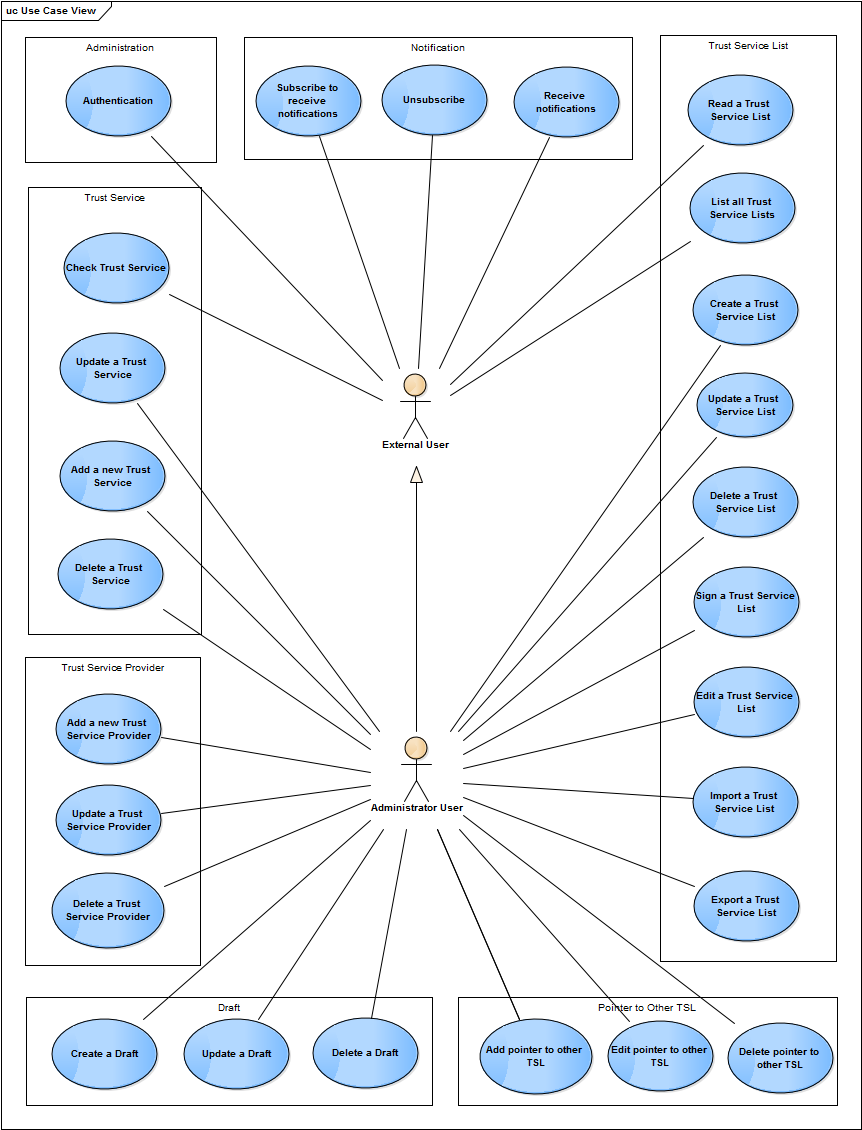
\includegraphics[scale=0.53]{figures/use-case-diagram}
	\caption{Diagramme de cas d'utilisation. Illustration adaptée de \textit{Design documentation}~\cite{design-document}}
	\label{fig:use-case-diagram}
\end{figure}
\clearpage

\subsection{Administration}
\subsubsection{Authentification}
L'authentification permet à un utilisateur d'être reconnu par le système comme étant administrateur, c'est-à-dire comme ayant droit d'éditer des listes de confiance. Cette fonctionnalité est gérée grâce à la blockchain, en effet les clés publiques des utilisateurs enregistrés en tant qu'administrateur sont sauvegardées dans la blockchain. Afin de s'authentifier, l'utilisateur doit utiliser sa clé privée.

\subsection{Trust Service List}
\label{sec:tsl}
\subsubsection{Créer une nouvelle Trust Service List}
Un utilisateur authentifié et autorisé peut créer une TSL pour un territoire donné. Pour cela, il doit créer une nouvelle TSL, remplir tous les champs requis de celle-ci, valider ces champs et enfin la signer. Ensuite, la liste complète est stockée et répliquée à travers les nœuds du réseau distribué et une nouvelle entrée est créée dans la blockchain afin de la référencer dans la gTSL.
\subsubsection{Lire les informations relatives à une Trust Service List}
Tout utilisateur peut lire et récupérer les informations relatives à une TSL existante afin d'en analyser le contenu. Le système permet d'effectuer une recherche en se basant sur différents critères comme par exemple le territoire, le type de service, le statut ou un certificat.
\subsubsection{Éditer une Trust Service List}
Un utilisateur authentifié et autorisé peut modifier une TSL. Ce processus est similaire à la création sauf que l'utilisateur n'a pas à saisir toutes les informations car la liste existante lui est fournie. Une édition peut donner lieu à l'ajout, la suppression ou la modification d'un TSP; l'ajout, la suppression ou la modification d'un TS; la modification d'un champ obligatoire; l'ajout, la suppression ou la modification d'un champ optionnel. Il est important de noter que lors d'une édition, l'utilisateur doit signer à nouveau la TSL.
\subsubsection{Supprimer une Trust Service List}
Un utilisateur authentifié et autorisé peut supprimer une TSL. Ce cas d'utilisation correspond à la révocation d'une TSL. Dans la pratique, une TSL n'est jamais supprimée définitivement, elle est simplement considérée comme révoquée et peut être possiblement réhabilitée.
\subsubsection{Lister toutes les Trust Service Lists}
Le système permet la récupération de l'ensemble des TSLs afin d'avoir une vue globale de la gTSL.
\subsubsection{Signer une Trust Service List}
Cette fonctionnalité permet aux utilisateurs authentifiés et autorisés de signer une TSL lors de la création ou d'une édition.
\subsubsection{Importer une Trust Service List}
Le système permet aux utilisateurs d'importer des TSLs au format XML afin de les créer ou les modifier dans la gTSL. Cela a pour intérêt d'une part de permettre une édition à la main des utilisateurs, d'autre part d'autoriser un système externe de créer des TSLs. Malgré cela, la TSL doit être valide afin d'être acceptée par le système. Cette fonctionnalité peut aussi être utile en cas de migration. Il est important de noter que le fichier XML doit être signé.
\subsubsection{Exporter une Trust Service List}
Le système permet aux utilisateurs d'exporter des TSLs au format XML. Cela pour intérêt de permettre à des systèmes externes de les manipuler et d'y appliquer des modifications. Cette fonctionnalité peut aussi être utile en cas de migration.

\subsection{Draft}
\subsubsection{Créer un brouillon de Trust Service List}
Le système permet aux utilisateurs de créer un brouillon\footnote{en anglais, draft.} d'une TSL. En effet, un utilisateur peut créer un brouillon d'une liste existante dans le but de la soumettre plus tard. Les brouillons sont stockés dans une base de données locale. Lorsque l'utilisateur considère son brouillon comme terminé et que le système l'a validé, le brouillon est alors poussé en production et remplace la liste actuelle. On peut assimiler ce fonctionnement à celui des emails, qui peuvent être enregistrés comme brouillon avant d'être envoyés.
\subsubsection{Éditer un brouillon de Trust Service List}
Le système permet aux utilisateurs d'éditer un brouillon qui a été enregistré localement mais qui n'a pas été soumis à la production.
\subsubsection{Supprimer un brouillon de Trust Service List}
Le système permet aux utilisateurs de supprimer un brouillon qui a été enregistré localement mais qui n'a pas été soumis à la production.

\subsection{Pointer to Other TSL}
\subsubsection{Ajouter un pointeur vers une autre TSL}
Dans l'architecture actuelle, il est possible d'ajouter à une TSL un pointeur vers une autre TSL. Un pointeur permet de référencer une liste dans une autre lorsque cela est pertinent. Afin de rester conforme au format actuel de Trust Service List, cette action doit être disponible dans la nouvelle implémentation.
\subsubsection{Éditer un pointeur vers une autre TSL}
Un utilisateur authentifié et autorisé peut modifier un pointeur d'une TSL. En effet, si une TSL est modifiée, il est possible que sa référence soit aussi modifiée.
\subsubsection{Supprimer un pointeur vers une autre TSL}
Un utilisateur authentifié et autorisé peut supprimer un pointeur d'une TSL. Dans le cas où il n'est plus pertinent de référencer une autre TSL, l'utilisateur peut supprimer le pointeur.

\subsection{Trust Service Provider}
\subsubsection{Ajouter un nouveau Trust Service Provider}
Un utilisateur authentifié et autorisé peut ajouter un TSP dans une TSL. Pour cela, il doit créer un nouveau fournisseur, remplir tous les champs requis pour celui-ci et valider ces champs. Le fournisseur doit obligatoirement proposer au minimum un service de confiance, car dans le cas contraire il ne serait pas pertinent de l'ajouter. La liste sera alors mise à jour. Il est important de noter que l'ajout d'un fournisseur est considéré comme une édition de la liste. Par conséquent, l'utilisateur doit signer à nouveau la TSL.
\subsubsection{Éditer un Trust Service Provider}
Un utilisateur authentifié et autorisé peut éditer un TSP dans une TSL. En effet, les informations d'un TSP peuvent être amenées à changer, l'utilisateur a donc la possibilité de les modifier. Une édition peut donner lieu à la modification du nom, de l'adresse électronique ou postale, de l'URI ou d'autres informations optionnelles du TSP. Tout comme l'ajout, l'édition d'un TSP est considérée comme une édition de la liste. Par conséquent, l'utilisateur doit signer à nouveau la TSL.
\subsubsection{Supprimer un Trust Service Provider}
Un utilisateur authentifié et autorisé peut supprimer un TSP d'une TSL. Par exemple, un TSP peut être supprimé s'il n'existe plus ou s'il ne répond plus aux critères de confiance. Tout comme l'ajout, la suppression d'un TSP est considérée comme une édition de la liste. Par conséquent, l'utilisateur doit signer à nouveau la TSL.

\subsection{Trust Service}
\subsubsection{Ajouter un nouveau Trust Service}
Un utilisateur authentifié et autorisé peut ajouter un TS à un TSP. Il est obligatoire que le TSP ait déjà été créé. Pour cela, il doit créer un nouveau service, remplir tous les champs requis pour celui-ci et valider ces champs. Il est important de noter que l'ajout d'un service est considéré comme une édition de la liste. Par conséquent, l'utilisateur doit signer à nouveau la TSL.
\subsubsection{Éditer un Trust Service}
Un utilisateur authentifié et autorisé peut éditer un TS d'un TSP. En effet, les informations d'un TS peuvent être amenées à changer, l'utilisateur a donc la possibilité de les modifier. Une édition peut donner lieu à la modification du nom, du statut, de l'URI ou d'autres informations du TS. Tout comme l'ajout, l'édition d'un TS est considérée comme une édition de la liste. Par conséquent, l'utilisateur doit signer à nouveau la TSL.
\subsubsection{Supprimer un Trust Service}
Un utilisateur authentifié et autorisé peut supprimer un TS d'un TSP. Par exemple, un TS peut être supprimé s'il n'est plus proposé par le fournisseur. Tout comme l'ajout, la suppression d'un TS est considérée comme une édition de la liste. Par conséquent, l'utilisateur doit signer à nouveau la TSL.
\subsubsection{Vérifier un Trust Service}
Le système permet aux utilisateurs externes de rechercher une 
trust anchor\footnote{Dans les systèmes cryptographiques à structure hiérarchique, une trust anchor est une autorité pour laquelle la confiance est assumée et non dérivée. Dans le cadre de l'architecture X.509, un certificat racine serait la trust anchor de laquelle toute la chaîne de confiance est dérivée.} 
à un moment donné. 
Une opération de recherche peut être effectuée en passant en paramètre un certificat ou le nom associé au service souhaité d'une TSL. La réponse contiendra les informations sur le service identifié.

\subsection{Notification}
\label{sec:notification}
\subsubsection{S'abonner pour recevoir des notifications}
Le système permet aux utilisateurs de s'abonner à des notifications concernant les listes de confiance. Par exemple, un utilisateur peut être notifié par email en cas de modification d'une liste donnée.
\subsubsection{Se désabonner}
Un utilisateur abonné à des notifications à la possibilité de se désabonner.
\subsubsection{Recevoir les notifications}
Le système doit envoyer des notifications à tous les utilisateurs abonnés à une liste donnée, lors de la mise à jour de celle-ci.

\section{Modules du système}
\label{sec:modules}

Cette section décrit la structure et les composants de haut niveau. La Figure~\ref{fig:highlevel-components} présente les différents modules.

\begin{figure}[h]
	\centering
	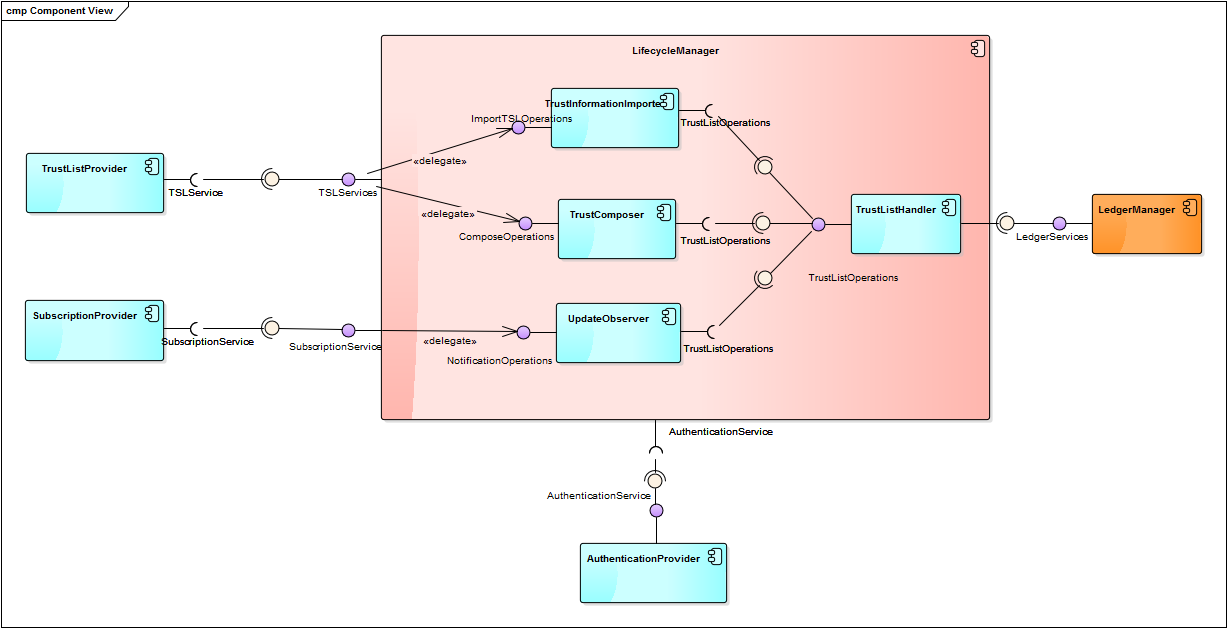
\includegraphics[scale=0.38]{figures/highlevel-components}
	\caption{Composants de haut niveau de la gTSL. Illustration extraite de \textit{Design documentation}~\cite{design-document}}
	\label{fig:highlevel-components}
\end{figure}

\subsection{Lifecycle Manager}

Ce composant est le cœur de la gTSL. Il fournit les fonctionnalités nécessaires à la gestion des listes de confiance et de leurs informations. Il est composé de quatre sous-composants:
\begin{itemize}
	\item \textit{TrustListHandler}, qui communique avec le \textit{Ledger Manager}, et expose les fonctionnalités requises à la création, l'édition, la suppression et la récupération des informations concernant les TSPs et les TSs conservées dans la gTSL;
	\item \textit{TrustInformationImporter}, qui fournit les fonctionnalités requises à l'import et à l'export de listes de confiance;
	\item \textit{UpdateObserver}, implémentant un design pattern Observer\footnote{Le design pattern (que l'on peut traduire par patron de conception) observateur est utilisé pour envoyer un signal à tous les observateurs lorsqu'une condition est remplie sur le module dit observé, la condition peut être par exemple la mise à jour d'une donnée.}, qui a pour rôle de notifier les utilisateurs abonnés lorsqu'un changement se produit sur la gTSL;
	\item \textit{TrustComposer}, qui gère la logique métier associée à la gestion des services de confiance et des certificats qualifiés.
\end{itemize}

De plus, le \textit{Lifecycle Manager} est interfacé avec des composants externes:
\begin{itemize}
	\item \textit{TrustListProvider}, qui gère les opérations relatives aux listes de confiance et qui est interfacé avec le \textit{Lifecycle Manager} à travers le \textit{TSLService};
	\item \textit{SubscriptionProvider}, qui est un composant externe interfacé avec le module \textit{UpdateObserver} à travers le \textit{SubscriptionService}, qui fournit aux abonnés des fonctionnalités de notifications;
	\item \textit{AuthenticationProvider}, qui traite les opérations d'authentification et qui est interfacé avec le \textit{Lifecycle Manager} à travers le \textit{AuthenticationService}.
\end{itemize}

\subsection{Ledger Manager}

Le\textit{ Ledger Manager} est le module qui gère toutes les interactions avec la solution de stockage sur laquelle repose la gTSL pour conserver les données. Ce module s'appuie sur une interface définissant les fonctions permettant de manipuler la solution de stockage de données.

\section{Processus métier}

Cette section contient des diagrammes permettant de décrire le comportement et les interactions des différents composants, modules et classes du logiciel. Les processus présentés sont les plus représentatifs des actions possibles sur la gTSL, mais ne représentent pas la totalité des processus.

\subsection{Édition d'une liste de confiance}

À travers le processus d'édition, un utilisateur d'administration peut effectuer des modifications sur une TSL spécifiée.
Ce processus est illustré dans le diagramme BPMN1.1\footnote{BPMN, acronyme anglais de Business process model and notation, est une représentation graphique pour spécifier les processus métier dans un modèle de processus métier.} dans la Figure~\ref{fig:edit-flow}.

\begin{figure}[h]
	\centering
	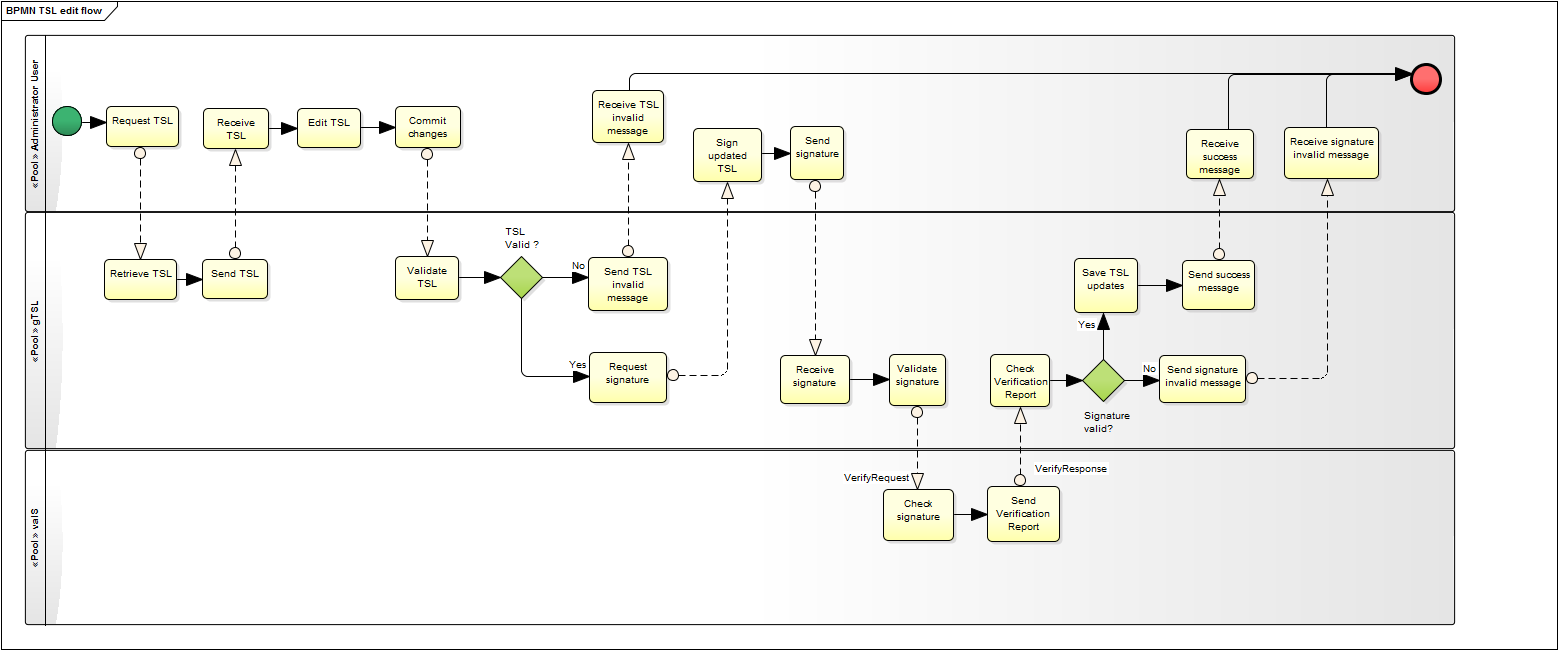
\includegraphics[scale=0.3]{figures/edit-flow}
	\caption{Édition d'une liste de confiance. Illustration extraite de \textit{Design documentation}~\cite{design-document}}
	\label{fig:edit-flow}
\end{figure}

\subsection{Import d'une liste de confiance}

À travers le processus d'import, un utilisateur d'administration peut importer une TSL dans la gTSL. À ce titre, un utilisateur d'administration peut soit importer une TSL existante, c'est-à-dire en téléchargeant un fichier de TSL, soit définir l'URL d'une TSL distante à inclure dans la gTSL. Ce processus est illustré dans le diagramme BPMN1.1 dans la Figure~\ref{fig:import-flow}.

\begin{figure}[h]
	\centering
	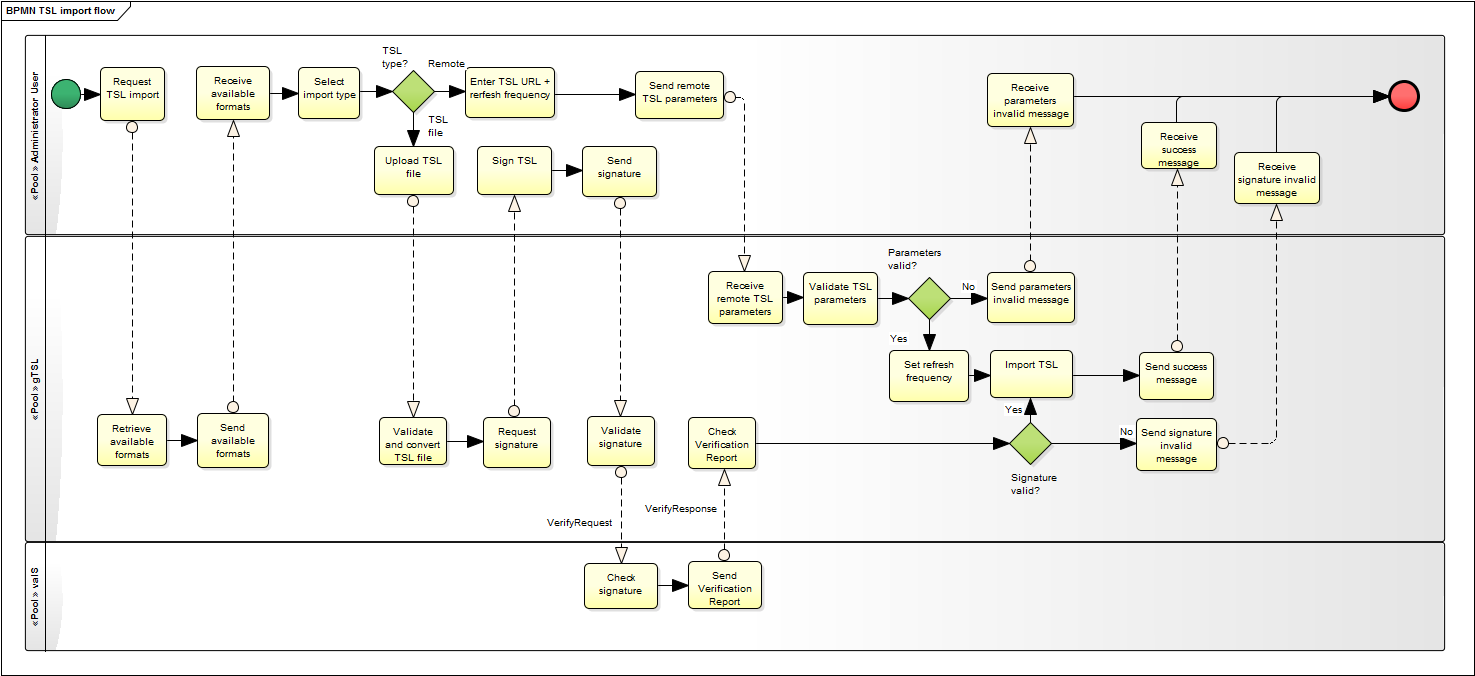
\includegraphics[scale=0.31]{figures/import-flow}
	\caption{Import d'une liste de confiance. Illustration extraite de \textit{Design documentation}~\cite{design-document}}
	\label{fig:import-flow}
\end{figure}

\subsection{Gestion des notifications}

À travers le processus de notifications, tous les utilisateurs peuvent souscrire aux notifications d'une TSL. Le système de notifications surveille les changements opérés sur la gTSL et informe les utilisateurs abonnés lorsque des modifications sont détectées. Ce processus est illustré dans le diagramme BPMN1.1 dans la Figure~\ref{fig:notification-flow}.

\begin{figure}[h]
	\centering
	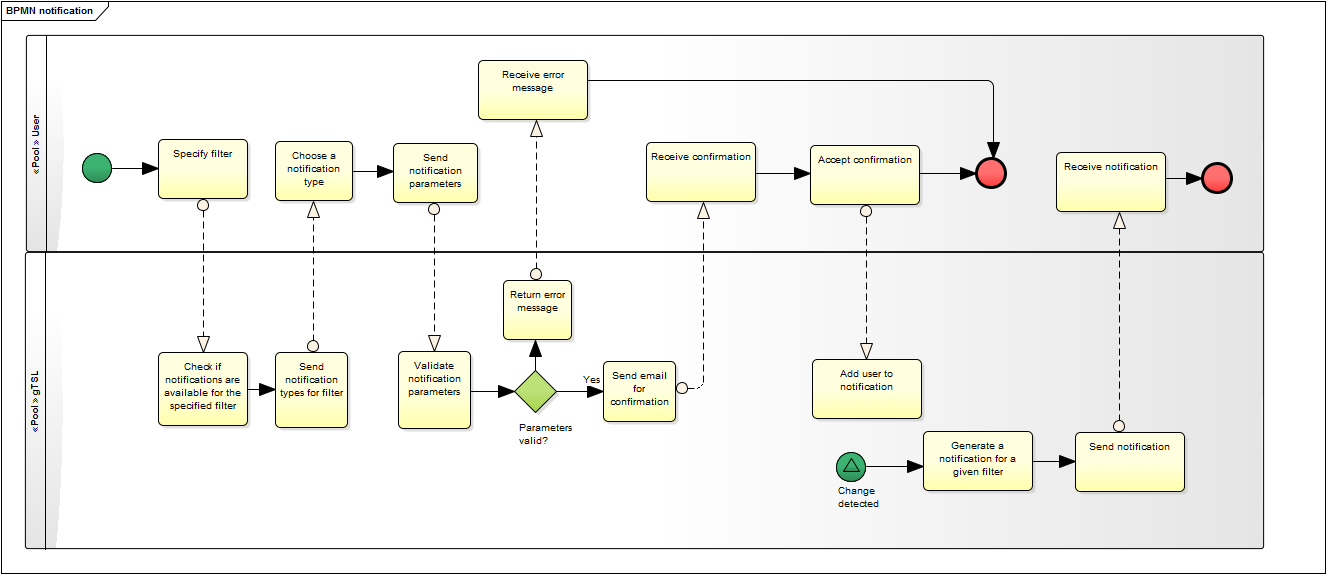
\includegraphics[scale=0.33]{figures/notification-flow}
	\caption{Gestion des notifications. Illustration extraite de \textit{Design documentation}~\cite{design-document}}
	\label{fig:notification-flow}
\end{figure}

\section{Modèle de données}

Cette section contient des diagrammes permettant de décrire les classes implémentées dans le logiciel. Le diagramme de classes UML fourni en Figure~\ref{fig:model} définit les structures de données de base pour les listes de confiance conformément à leur définition dans ETSI TS 119 612~\cite{ETSITS119612}.

\begin{figure}[h]
	\centering
	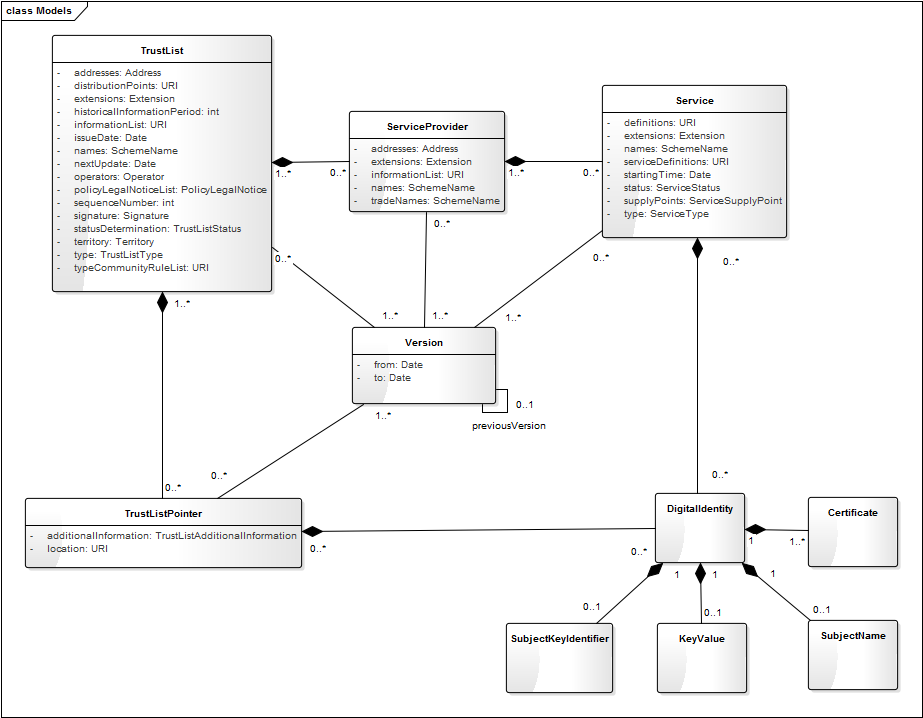
\includegraphics[scale=0.51]{figures/model}
	\caption{Diagramme de classes simplifié. Illustration extraite de \textit{Design documentation}~\cite{design-document}}
	\label{fig:model}
\end{figure}

Les principales entités sont:
\begin{itemize}
	\item \textit{TrustList}, qui définit la liste de confiance pour un territoire donné;
	\item \textit{TrustListPointer}, qui est lié uniquement aux listes de confiance des États membres et utilisé uniquement pour la LoTL;
	\item \textit{ServiceProvider}, qui contient les informations d'un fournisseur de services;
	\item \textit{Service}, qui définit un service métier pour un fournisseur identifié par un ensemble d'identités numériques;
	\item \textit{Version}, qui rassemble les informations concernant l'historique de la liste de confiance et des entités associées.
\end{itemize}
\clearpage

Le modèle de données peut être simplifié par un graphe orienté, comme le montre la Figure~\ref{fig:dependencies}, où les nœuds représentent les entités et les arrêtes représentent les relations entre ces entités.

\begin{figure}[h]
	\centering
	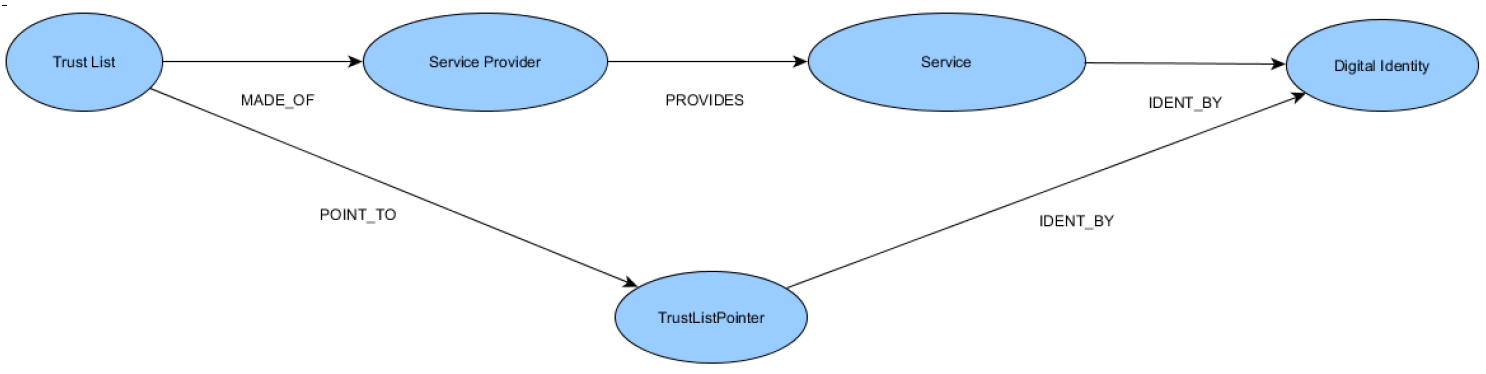
\includegraphics[scale=0.42]{figures/dependencies}
	\caption{Graphe de dépendances des données. Illustration extraite de \textit{Design documentation}~\cite{design-document}}
	\label{fig:dependencies}
\end{figure}

\chapter{Réalisation de la solution proposée}
\label{chap:realisation}

Dans ce chapitre, nous détaillons l'architecture mise en place ainsi que l'implémentation des modules présentés au Chapitre~\ref{chap:analyse}. Ce chapitre présente aussi la solution et les validations qui ont été effectuées.

\section{Architecture mise en place}
\label{sec:architecture}

Cette partie concerne l'architecture du système et différencie d'une part l'architecture d'un nœud de la gTSL et d'autre part l'architecture globale du système. La première vision permet de détailler au niveau local les différents composants utilisés. La seconde vision permet de comprendre au niveau général la décentralisation et la distribution des informations à travers un réseau de multiples nœuds interconnectés de la gTSL, agissant dans un but commun.

Cette section présente uniquement l'architecture logicielle du service de gTSL mais ne fournit pas la documentation de la mise en place technique du système. Des explications concernant le déploiement du système (outils utilisés, processus d'installation, etc.) sont détaillées dans le document GTSL - Project Setup Documentation disponible en Annexe~\ref{anx:gtsl-setup}. J'ai eu pour mission de rédiger ce document dans le but de fournir une précision sur le déploiement du module de gTSL. Néanmoins, ce document ne correspond pas au manuel d'installation utilisateur qui fait l'objet d'un second document intitulé GTSL - Project Setup Guidelines disponible en Annexe~\ref{anx:gtsl-guidelines} que j'ai également rédigé.

\subsection{Architecture d'un nœud de la gTSL}

Le système mis en place est composé de deux parties principales. La première partie est une interface d'administration qui permet aux utilisateurs authentifiés d'opérer facilement des modifications sur la gTSL à l'aide d'une interface graphique. La seconde partie est un nœud de la gTSL qui contient un serveur d'applications, une base de données locale, une instance connectée au réseau IPFS et une instance connectée à la blockchain Ethereum. Ces deux parties communiquent via le protocole HTTP. Les données que contiennent les requêtes échangées sont formatées en JSON. Il est important de noter que l'interface d'administration peut être omise dans le cas où le nœud est déployé à des fins de consultation de la gTSL par des utilisateurs externes uniquement. La Figure~\ref{fig:architecture-node} présente les interactions entre ces différents composants.
\clearpage

\begin{figure}[h]
	\centering
	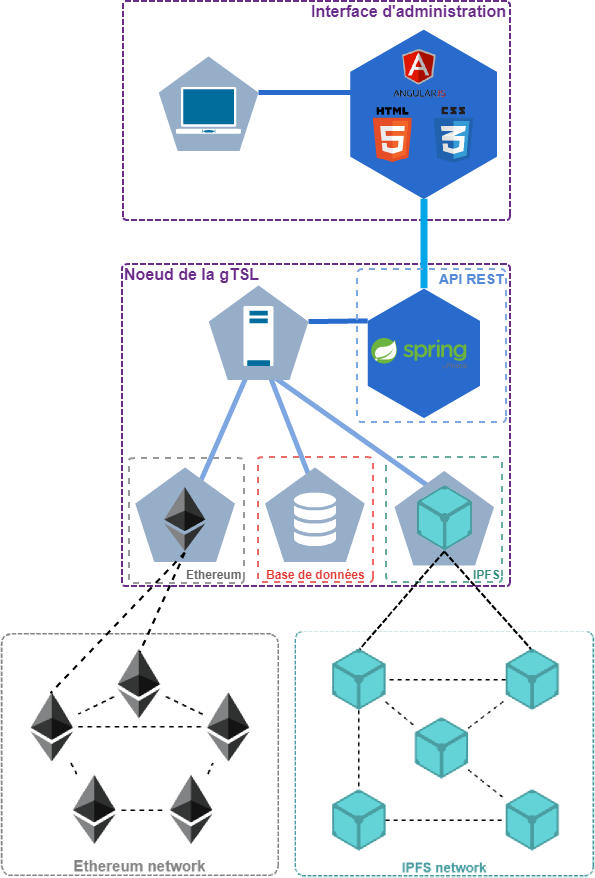
\includegraphics[scale=0.42]{figures/architecture}
	\caption{Architecture du système}
	\label{fig:architecture-node}
\end{figure}

\subsubsection{Interface d'administration}

L'interface d'administration fournit une interface web graphique aux utilisateurs d'administration afin qu'ils puissent gérer la gTSL. Il est développé avec les technologies HTML5, CSS3 et AngularJS. Dans le cadre de ce projet, nous avons décidé de réutiliser l'interface existante, appelée TL Manager. Cette interface permet notamment aux utilisateurs de créer des drafts qui peuvent ensuite être publiés dans la gTSL. Néanmoins, il n'est pas détaillé dans ce mémoire puisqu'il n'entre pas dans le cadre du stage.

\subsubsection{Interface de programmation applicative REST}

L'API\footnote{Une API, acronyme anglais de Application Programming Interface, est une interface de programmation applicative qui a pour but de fournir des services à d'autres logiciels.} REST expose des web services fournissant toutes les opérations nécessaires à la gestion de la gTSL. Il a été développé en Java en s'appuyant sur le framework Spring. Cette interface de programmation encapsule les différents modules introduits en Section~\ref{sec:modules} permettant de gérer les données, d'authentifier les utilisateurs et de s'abonner aux listes de confiance. Elle est décomposée en trois parties et présentée dans la Figure~\ref{fig:rest-api}.

\begin{figure}[h]
	\centering
	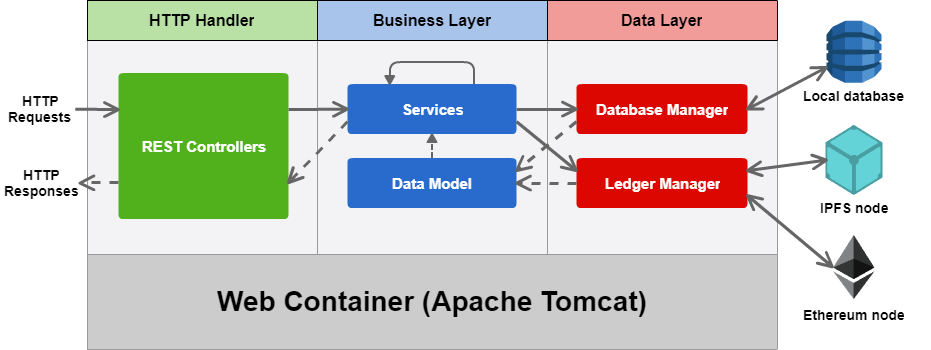
\includegraphics[scale=0.52]{figures/rest-api}
	\caption{Interface de programmation applicative}
	\label{fig:rest-api}
\end{figure}

Le \textit{HTTP Handler}\footnote{en français, gestionnaire HTTP.} a pour rôle d'intercepter et de répondre aux requêtes HTTP. Il est composé de multiples contrôleurs chargés de faire appel à des services qui traitent les demandes des utilisateurs. Chaque contrôleur est défini sur une URL précise et expose des méthodes dans lesquelles sont configurés la méthode HTTP à utiliser ainsi que l'en-tête et le corps de la requête. Le \textit{HTTP Handler} renvoie des réponses HTTP contenant un statut permettant de déterminer le résultat d'une requête ou d'indiquer au client une erreur. Si aucune erreur n'est survenue, le code de réponse HTTP 200 OK est envoyé.

La \textit{Business Layer}\footnote{en français, couche métier.} est la partie traitement des données de l'application. C'est dans cette partie que les données sont vérifiées, validées, transformées ou éventuellement rejetées si elles sont invalides. Elle est composée de services qui sont appelés par les contrôleurs REST. Les services font appel à la couche de données afin de lire, modifier ou
écrire dans la base de données. Ils peuvent aussi faire appel à d'autres services si cela est nécessaire. Dans cette partie sont gérées les éventuelles erreurs et exceptions qui peuvent survenir lors du traitement des données.

La partie \textit{Data Layer}\footnote{en français, couche de données.} a pour objectif de gérer les données. La couche de données est composée d'une part du \textit{Database Manager} et d'autre part du \textit{Ledger Manager}. Le \textit{Database Manager} a pour rôle de gérer les insertions, les mises à jour et les récupérations des données concernant les abonnements et les drafts en utilisant la base de données locale. Le \textit{Ledger Manager} quant à lui joue le rôle d'interface entre le nœud IPFS et le nœud Ethereum, il a aussi à charge de gérer les données liées aux listes de confiance.

\subsubsection{Nœud IPFS}

Le nœud IPFS est connecté à un réseau pair-à-pair composé d'autres nœuds IPFS anonymes. Il a pour rôle de maintenir les données dans ce réseau en les répliquant à travers les autres nœuds IPFS appartenant au service de gTSL, ce qui forme ce que l'on appelle un cluster\footnote{Un cluster est un ensemble de serveurs sur un réseau qui agissent dans un but commun.}. Le nœud interagit avec le système via le \textit{Ledger Manager} qui est chargé de lui communiquer les données à stocker.

\subsubsection{Nœud Ethereum}

Le nœud Ethereum est connecté à un réseau pair-à-pair composé d'autres nœuds Ethereum anonymes. Il a pour rôle d'assurer l'intégrité des données grâce au consensus de la blockchain. Le nœud s'interface avec le \textit{Ledger Manager} à qui il doit fournir l'état courant de la gTSL stocké dans un smart contract. L'état courant correspond à l'ensemble des hashes représentatifs de chaque liste de confiance. Son deuxième rôle est la gestion des utilisateurs. En effet, l'authentification est gérée par un smart contract qui maintient les clés publiques des personnes autorisées à modifier la gTSL.

\subsubsection{Base de données}

La base de données locale à chaque nœud a pour but de stocker les emails des personnes abonnées aux notifications ainsi que les drafts de listes de confiance. Les notifications sont donc gérées par le nœud auquel l'utilisateur a souscrit. L'intérêt de conserver les emails dans une base de données locale est de ne pas diffuser publiquement ces emails, ce qui serait le cas si ils étaient stockés dans la blockchain, afin de respecter la vie privée des utilisateurs. Concernant les drafts, on les stocke ni dans IPFS ni dans Ethereum mais bien dans une base de données locale. En effet, on ne veut pas rendre public un draft puisqu'il peut être incomplet ou contenir des informations non vérifiées. De plus, il n'est pas pertinent de s'assurer de la validité des données d'un draft puisqu'il n'est pas rendu public. Les utilisateurs d'administration de la gTSL doivent dans tous les cas déployer leur propre instance du nœud de gTSL comme expliqué en introduction de la Section~\ref{sec:architecture}, ils auront donc leur base de données dédiée contenant uniquement les drafts qu'ils ont établis.

\subsection{Architecture globale}

Le système présenté en Figure~\ref{fig:architecture-node} sera déployé par tous les utilisateurs d'administration dans toute l'Europe et au-delà. En effet, chaque administrateur a besoin de son propre compte Ethereum, c'est-à-dire de son propre nœud Ethereum et de son propre identifiant de nœud IPFS, c'est-à-dire de son propre nœud IPFS. Cela permet d'augmenter le nombre de duplications des données et donc d'améliorer la résilience du système. De plus, il est envisagé de mettre en place des instances publiques afin que les utilisateurs externes puissent récupérer les données liées à la gTSL. Dans ce cas, l'interface d'administration n'est pas nécessaire. Ce système est open-source, cela implique que toute personne souhaitant déployer sa propre instance aura la possibilité de le faire. Malgré tout, il ne lui est pas possible de modifier la gTSL puisqu'il ne dispose pas des autorisations requises. Toutes ces instances forment ensemble un système décentralisé et distribué qui permet de maintenir l'entièreté des données. 

La Figure~\ref{fig:architecture-global} présente l'architecture globale du système, décentralisée et distribuée, composée de plusieurs nœuds de la gTSL. Certains composants ne jouant aucun rôle dans la décentralisation du modèle, ils ont été retirés des nœuds de gTSL dans un soucis de compréhension.
\clearpage

\begin{figure}[h]
	\centering
	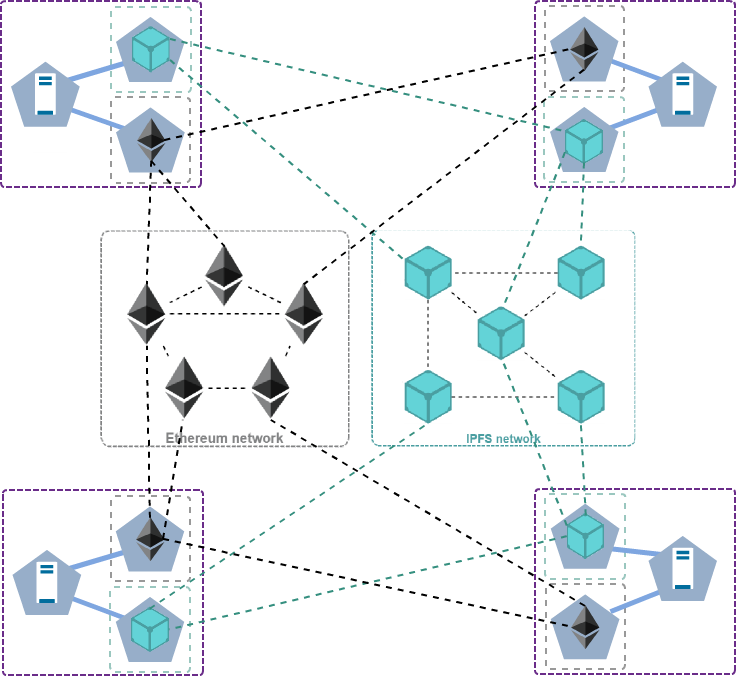
\includegraphics[scale=0.58]{figures/architecture-global}
	\caption{Architecture globale}
	\label{fig:architecture-global}
\end{figure}

On observe dans la Figure~\ref{fig:architecture-global} que la décentralisation se fait d'une part via le réseau IPFS qui maintient les données et d'autre part via le réseau Ethereum chargé de conserver l'état courant de la gTSL dans la blockchain. Il est aussi important de noter que ces réseaux sont publics, ils existent donc d'autres nœuds anonymes, non engagés au niveau de la gTSL, mais qui participent tout de même à la résilience du système.

\section{Implémentation des modules}

Cette section présente les différents modules de la gTSL, et plus particulièrement les modules permettant de stocker les données, d'authentifier les utilisateurs, de gérer les notifications et de manipuler les listes de confiance.

\subsection{Ledger Manager}
\label{sec:realisation-ledger}

Dans cette section est décrite la manière d'intégrer Ethereum et IPFS. Dans un premier temps est exposé l'intérêt d'utiliser ces technologies ensemble. Ensuite est présentée la structure de données mise en place afin de les interfacer. Enfin est détaillé le système implémenté afin de gérer l'historique des versions de la gTSL.

Les explications fournies dans cette partie sont tirées du document Integration of Ethereum \& IPFS disponible en Annexe~\ref{anx:ipfs-ethereum} que j'ai rédigé dans le but de fournir une explication de l'utilisation de technologies décentralisées et distribuées dans le cadre du module de gTSL.

\subsubsection{L'avantage de coupler IPFS \& Ethereum}

Un moyen simple de stocker les données de la gTSL est de les conserver dans une blockchain, cela évite la mise en place d'un système de fichiers décentralisé. 
Bien qu'une blockchain présente beaucoup d'avantages, elle présente également des inconvénients.
L'un d'eux est que le déploiement d'un smart contract dans la blockchain Ethereum doit être payé.
De plus, le prix augmente proportionnellement avec la taille du smart contract, c'est-à-dire son nombre d'opérations et la taille des données qu'il contient.
Ainsi, le prix suit la quantité de données stockées.
Une façon de réduire le coût est d'utiliser un réseau distribué afin de stocker les données de la gTSL et d'utiliser une blockchain afin de maintenir l'état des données.
Dans IPFS, toutes les données sont adressées par leur hash, ce qui rend leur état facilement maintenable. Par conséquent, pour toutes les données d'une TSL, la blockchain ne maintient qu'un hash correspondant à l'état actuel de ces données. Cette solution réduit considérablement les coûts d'utilisation de la blockchain.

\subsubsection{L'intégration des technologies}

Comme expliqué dans la partie précédente, seul le hash des données est stocké dans la blockchain.
Toutes les données réelles sont stockées dans IPFS, désigné comme étant la {\em couche de données}\footnote{en anglais, Data layer}. 
Un hash est l'adresse qui identifie une TSL donnée. 
Par conséquent, lorsqu'une TSL est stockée dans IPFS, un hash unique est automatiquement calculé à partir de ses données. 
Ce hash est ensuite stocké dans un smart contract dans lequel il est rattaché à un identifiant unique non mutable de la TSL, correspondant au code du pays de la TSL conformément au standard ETSI TS 119 612~\cite{ETSITS119612}.
Cet identifiant non mutable est ensuite utilisé par le système pour retrouver le hash d'une TSL.
Contrairement à l'identifiant non mutable d'une TSL, le hash d'une TSL dépend des données qu'elle contient et est donc mutable. 
Plus particulièrement le hash est recalculé à chaque édition de la TSL par un État membre.
La blockchain enregistre l'état courant des TSLs et met à jour l'état du contrat, on la désigne donc comme étant la {\em couche d'états}\footnote{en anglais, State layer}. 
Le smart contract maintient l'état de chaque TSL et permet aux utilisateurs d'ajouter, de mettre à jour, de supprimer ou de récupérer une TSL.
Il est important de noter qu'une autorisation est nécessaire pour appliquer des changements à une TSL mais que la lecture est disponible publiquement.

Une abstraction de la mise en œuvre du smart contract écrit en langage Solidity est fournie dans le Listing~\ref{lst:ledgerContract}.

\clearpage
\begin{lstlisting}[language=solidity, basicstyle=\small, caption={Ledger Contract}, label={lst:ledgerContract}]
contract Ledger {
	
	// Attributes
	mapping(bytes32 => bytes) public gtsl;
	
	function addTsl(bytes32 _code, bytes _hash)
		public onlyAuthorized
	{
		gtsl[_code] = _hash;
	}
	
	function updateTsl(bytes32 _code, bytes _hash)
		public onlyAuthorized
	{
		gtsl[_code] = _hash;
	}
	
	function removeTsl(bytes32 _code)
		public onlyAuthorized
	{
		delete gtsl[_code];
	}
	
}
\end{lstlisting}

À noter qu'une fonction de récupération {\em get} est automatiquement générée par le compilateur pour chaque attribut. Le mot-clé {\em public} signifie que la fonction est accessible depuis l'extérieur du contrat, mais ne signifie pas que tous les utilisateurs ont la possibilité de l'exécuter. Le mot-clé {\em onlyAuthorized} définit que seul les personnes autorisées ont la possibilité de l'exécuter. La fonction {\em onlyAuthorized} est ce qu'on appelle un modificateur, il a pour rôle de filtrer l'exécution de la fonction en se basant sur les conditions d'exécution qu'il définit. Le modificateur {\em onlyAuthorized} est présenté dans le contrat de gestion des utilisateurs en Section~\ref{sec:authentication}.

\subsubsection{Gestion des versions}

Comme spécifié dans les besoins du service de gTSL, un historique de chaque TSL doit être conservé. 
Pour ce faire, l'idée est de maintenir une liste chaînée de toutes les versions de chaque TSL.
Cette liste chaînée est stockée dans IPFS et chaque version, que l'on appellera {\em commit}, de la liste peut être considérée comme un objet JSON, défini dans le Listing~\ref{lst:commitObject}.

\begin{lstlisting}[language=json, basicstyle=\small, caption={Commit Object}, label={lst:commitObject}]
{
	"dataAddress": "QmXXXXXXXXXXXXXX",
	"parent": "QmYYYYYYYYYYYYYY",
	"author": "Ada Lovelace ada@lov.cc",
	"date": "Mon July 24 15:19:12",
	"signature": {"signature info"}
}
\end{lstlisting}

Chaque attribut présent dans le Listing~\ref{lst:commitObject} est détaillé ci-dessous:
\begin{enumerate}
	\item \textit{dataAddress} est l'adresse (hash) IPFS pointant les données de la TSL pour la version actuelle;
	\item \textit{parent} est l'adresse (hash) IPFS pointant la version (commit) précédente de la TSL;
	\item \textit{author} identifie l'utilisateur qui a mis à jour la TSL;
	\item \textit{date} représente l'horodatage du commit;
	\item \textit{signature} sont des informations concernant la signature de l'utilisateur.
\end{enumerate}

Au lieu de sauvegarder le hash des données dans la blockchain, le hash de l'objet de commit est sauvegardé. L'objet commit encapsule le hash des données, le hash de l'objet commit de la version précédente et d'autres informations complémentaires. 
Cela permet à l'utilisateur de récupérer les données de la TSL, de savoir qui est l'utilisateur qui l'a créée et le moment où elle a été créée, et d'accéder à la version précédente. 
Cette couche supplémentaire au dessus des données contenant des méta-données de la version est désignée comme étant la {\em couche de méta-données}\footnote{en anglais, Meta-data layer}.

\subsubsection{Résultat}

La Figure~\ref{fig:versioning} résume la gestion de versions et l'intégration d'Ethereum \& IPFS.

\clearpage

\begin{figure}[h]
	\centering
	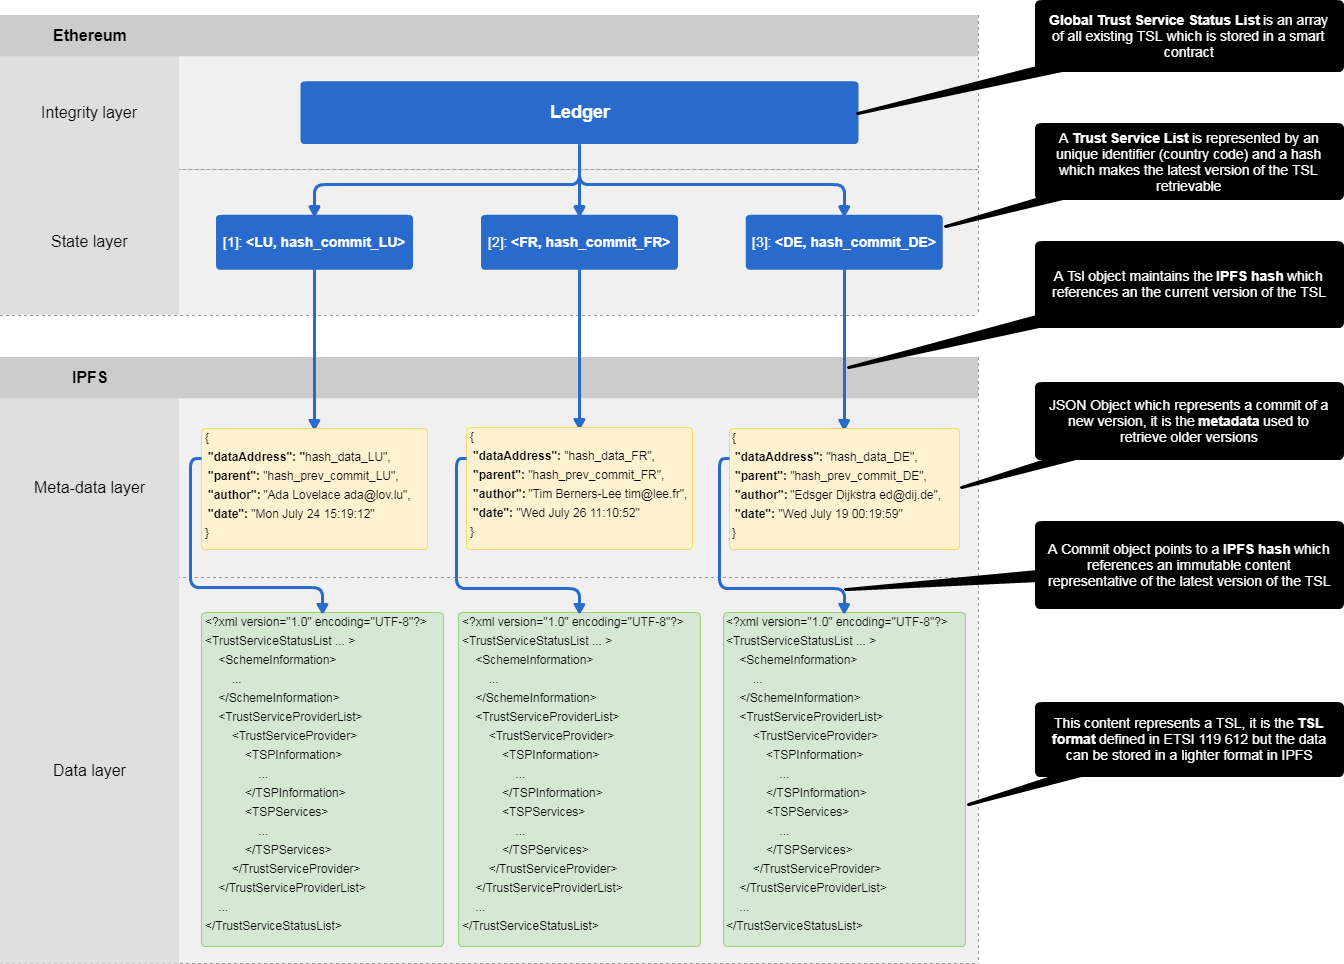
\includegraphics[scale=0.35]{figures/versioning}
	\caption{Ledger Manager. Illustration extraite de \textit{Integration of Ethereum \& IPFS}~\cite{ipfs-ethereum}}
	\label{fig:versioning}
\end{figure}

\subsection{Authentication Provider}
\label{sec:authentication}

Dans cette section sont décrits le service dédié à l'authentification et la gestion des utilisateurs. Dans un premier temps est exposé le processus d'authentification des utilisateurs. Ensuite est détaillé le processus de gestion des utilisateurs. Enfin est présenté le smart contract déployé dans la blockchain Ethereum, utilisé dans le but de réaliser ces actions.

\subsubsection{Authentification des utilisateurs}

L'authentification des utilisateurs est nécessaire uniquement pour les administrateurs de la gTSL. Le processus implémenté se détache du modèle classique d'authentification par nom d'utilisateur et mot de passe, qualifié d'authentification à un facteur. À la place, il repose sur une infrastructure à clés publiques qui permet d'authentifier les utilisateurs grâce à un certificat électronique, on qualifie cette authentification comme étant à deux facteurs. Afin de s'authentifier, l'utilisateur utilise sa clé privée, qui vérifiée contre sa clé publique permet de l'identifier.

Dans la pratique, l'authentification se fait via un smart contract déployé dans la blockchain Ethereum. Chaque utilisateur utilisant cette blockchain est identifié sur cette dernière grâce à une paire de clés.
Dans Ethereum, et dans la technologie blockchain en général, lorsqu'un utilisateur émet une transaction, il la signe à l'aide de sa clé privée et fournit la clé publique dans le corps de la transaction. Cette clé publique peut être récupérée dans le smart contract, afin de répertorier les utilisateurs autorisés à procéder à des modifications de la gTSL. 
Le smart contract maintient la liste des clés publiques des utilisateurs autorisés. 
Lorsqu'un utilisateur souhaite accéder à une fonctionnalité qui requiert une autorisation spécifique, le système va vérifier que sa clé publique est bien présente dans le smart contract de gestion des utilisateurs. Si sa clé publique est bien présente dans la liste des utilisateurs autorisés, alors le smart contract exécute la fonction appelée, sinon il refuse l'accès à cette fonction.

\subsubsection{Gestion des utilisateurs}

Cette section concerne uniquement les utilisateurs d'administration. En effet les utilisateurs externes ne sont pas concernés par l'authentification.
La gestion des utilisateurs concerne le processus par lequel des administrateurs peuvent être ajoutés ou révoqués de la liste des utilisateurs autorisés à modifier la gTSL et à gérer les utilisateurs. 
En opposition avec un modèle classique, le modèle conçu ne repose pas sur un "super-administrateur" qui a le pouvoir de gérer les administrateurs. 
%Dans notre modèle, tous les administrateurs ont les mêmes pouvoirs et aucun d'entre eux n'a la possibilité d'ajouter ou de retirer un utilisateur de la liste par son unique décision.

Le système mis en place est basé sur un service de votes déployé dans la blockchain Ethereum. Les actions de gestion des utilisateurs reposent sur un consortium d'administrateurs ayant la possibilité de soumettre une proposition d'ajout ou de révocation d'un membre. Pour cela, l'utilisateur établit une proposition de votes, en précisant l'action à effectuer (ajout/suppression), le membre concerné par le vote ainsi que la date limite du vote. Pour une proposition donnée, chaque administrateur a la possibilité de voter en faveur ou en défaveur. En outre, tous les membres du consortium disposent du droit de vote et ce vote a le même poids pour chacun d'entre eux, il n'existe aucun privilège pour un votant.

L'avantage majeur de cette conception est que le système ne peut être altéré par un seul et unique utilisateur malhonnête, puisqu'il est nécessaire que la proposition soit validée par la majorité du consortium. Le seul moyen pour un attaquant de corrompre le système ou d'en prendre le contrôle est de réussir à être majoritaire dans le consortium. Pour cela, il faudrait soit qu'il réussisse à dérober les clés privées de plus de la moitié du consortium, soit qu'il réussisse à ajouter des clés publiques qu'il détient dans la liste des clés autorisées, à hauteur d'au moins le nombre de clés déjà présentes dans la liste pour devenir majoritaire. 

Afin de renforcer la sécurité du système et de le protéger des attaques Sybil, il est possible d'imaginer que l'on ne se base pas sur la majorité (50\%) pour accepter la proposition mais sur un pourcentage plus élevé (80\% par exemple). En effet, les actions d'ajout ou de suppression d'un administrateur du consortium sont décidées oralement entre les États membres, avant même que l'opération ne soit saisie dans le module de gTSL. L'intérêt d'augmenter la majorité d'une proposition est de protéger davantage le système. De plus, dans le but d'empêcher qu'un utilisateur puisse valider un vote tout seul, une proposition doit atteindre un quorum pour être validée. Ce quorum, tout comme le seuil de majorité, peut être augmenté afin d'améliorer la sécurité du système.

Pour une proposition, on différencie trois résultats possibles:
\begin{itemize}
	\item succès, le consortium a approuvé la proposition car le quorum a été réuni, la majorité a voté en faveur de la proposition et la date limite est dépassée, le système procède donc à l'exécution de la proposition;
	\item annulé, la date limite est dépassée mais le quorum n'a pas été réuni, le système abandonne l'exécution;
	\item échec, la date limite est dépassée et le quorum a été réuni, mais la majorité a voté en défaveur de la proposition, le système abandonne l'exécution.
	\newline
\end{itemize}

La Figure~\ref{fig:user-flow} détaille le processus mis en place dans le cadre d'une proposition de votes initiée par un administrateur.

\begin{figure}[h]
	\centering
	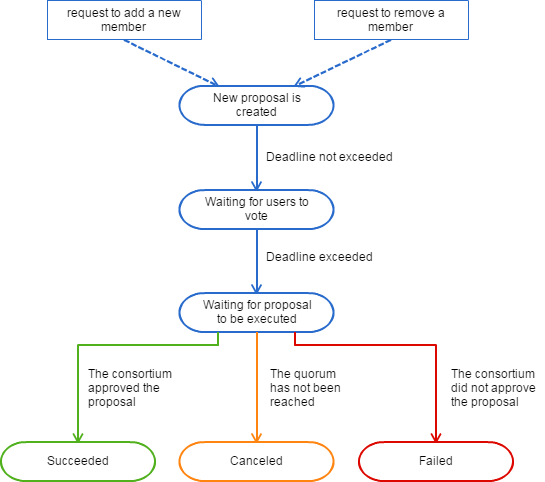
\includegraphics[scale=0.7]{figures/user-management-flow}
	\caption{Processus de gestion d'une proposition de votes}
	\label{fig:user-flow}
\end{figure}

\subsubsection{Implémentation}

Une abstraction de la mise en œuvre du smart contract est fournie dans le Listing~\ref{lst:consortiumContract}. Le code présenté a été simplifié dans un souci de compréhension et ne représente pas l'ensemble du smart contract implémenté.

\begin{lstlisting}[language=solidity, basicstyle=\small, caption={Consortium Contract}, label={lst:consortiumContract}]
contract Consortium {

	// Structures
	struct Member {
		bool authorized;
	}	
	struct Proposal {
		address member;
		function (address) action;
		mapping (address => bool) hasVoted;
		bool[] votes;
		bool result;
		uint deadline;
	}

	// Attributes
	mapping (address => Member) public members;
	Proposal[] proposals;

	// Modifiers
	modifier onlyAuthorized {
		require(members[msg.sender].authorized); _;
	}

	function requestAddMember(address _targetMember, uint _duration)
		public onlyAuthorized returns (uint proposalID)
	{
		return newProposal(_targetMember, addMember, _duration);
	}

	function requestRemoveMember(address _targetMember, uint _duration)
		public onlyAuthorized returns (uint proposalID)
	{
		return newProposal(_targetMember, removeMember, _duration);
	}

	function vote(uint _proposalID, bool _inSupport)
		public onlyAuthorized
	{
		Proposal storage p = proposals[_proposalID];
		require(now < p.deadline && !p.hasVoted[msg.sender]);
		p.hasVoted[msg.sender] = true;
		p.votes.push(_inSupport);
	}

	function executeProposal(uint _proposalID)
		public onlyAuthorized returns (bool)
	{
		Proposal storage p = proposals[_proposalID];
		require(now >= p.deadline);
		
		/* minimum quorum not reached */
		if (p.votes.length*100 < quorum) { 
			p.result = false;
		} else {		
			/* marjority algorithm, not provided here*/
			p.result = votesFor > votesAgainst;
		}

		/* execute action */
		if (p.result) {
			p.action(p.member);
		}
		
		return p.result;
	}
}
\end{lstlisting}

Les fonctions définies dans le Listing~\ref{lst:consortiumContract} sont détaillées ci-dessous:
\begin{itemize}
	\item \textit{onlyAuthorized} est un modificateur qui s'applique aux fonctions ayant pour but de vérifier que l'utilisateur appelant la fonction est répertorié dans la liste des administrateurs;
	\item \textit{requestAddMember} permet de créer une proposition d'ajout d'un nouvel administrateur;
	\item \textit{requestRemoveMember} permet de créer une proposition de révocation d'un administrateur;
	\item \textit{vote} permet aux utilisateurs d'administration d'appliquer leur vote à une proposition non expirée;
	\item \textit{executeProposal} permet de vérifier les votes d'une proposition expirée dans le but d'exécuter l'action associée si la proposition a été approuvée.
\end{itemize}

\subsection{Subscription Provider}

Le service d'abonnement possède trois fonctions qui sont l'abonnement, le désabonnement et la notification. Ce module est similaire à un service de newsletter\footnote{Une lettre d'information, newsletter en anglais, est un document d'information transmis par courrier électronique à l'ensemble des abonnés qui y ont souscrit.} que proposent de nombreux sites marchands par exemple.

\subsubsection{Abonnement}

Tout utilisateur a la possibilité de souscrire au service d'abonnement de la gTSL. Pour cela, il lui suffit de fournir son adresse email et de sélectionner les pays pour lesquels il souhaite être notifié. Ces informations sont stockées par le système dans une base de données locale au nœud de souscription. Cela signifie que l'utilisateur est abonné à un nœud en particulier.

\subsubsection{Désabonnement}

Tout utilisateur abonné à une TSL a la possibilité de se désabonner du service de notifications. Pour cela, il lui suffit de cliquer sur le lien de désabonnement dans un des emails de notification qu'il a pu recevoir. Il sera alors désabonné de son nœud de souscription.

\subsubsection{Notification}

Le système a pour mission de notifier tous les abonnés aux TSLs. Lorsqu'une modification est effectuée, alors tous les nœuds en sont informés. Chaque nœud doit donc extraire dans la base de données la liste des personnes ayant souscrit à la TSL modifiée et se charge ensuite de les en informer par email.

\subsection{Lifecycle Manager}

Le \textit{Lifecycle Manager} a pour rôle de gérer le cycle de vie des TSLs. Il se charge de traiter, vérifier et valider les informations relatives aux TSLs, on dit qu'il applique la logique métier. Ce module permet d'une part de gérer les TSLs et d'autre part de gérer les drafts. Concernant les TSLs, il permet de traiter la validation de tous les champs de la TSL conformément au standard ETSI TS 119 612~\cite{ETSITS119612} lors de l'ajout ou de l'édition. Il offre aussi la possibilité de procéder à des recherches sur les TSLs, d'importer une TSL au format XML et d'exporter une TSL au format XML. Les différentes techniques de recherche envisagées sur la gTSL sont évoquées dans le document gTSL Search Engine disponible en Annexe~\ref{anx:gtsl-search-engine}. Concernant les drafts, il gère le processus de création et d'édition des drafts en indiquant pour chacun quels champs sont valides vis-à-vis du standard ETSI TS 119 612~\cite{ETSITS119612}. Un draft peut être enregistré même s'il n'est pas valide, mais dans ce cas il ne pourra pas être publié dans la gTSL. À noter que les utilisateurs externes peuvent créer des drafts mais ne disposent pas des droits nécessaires pour publier les TSLs. Si un utilisateur externe est promu administrateur par la suite, il pourra tout de même publier les drafts réalisés en tant qu'utilisateur externe.

\section{Présentation de la solution}

Cette section concerne uniquement l'interface de programmation applicative. L'interface graphique d'administration a été réalisée dans la version antérieure du service de gestion des listes de confiance et sera réutilisée sans modifications majeures dans le cadre de la gTSL. Cette interface n'entre donc pas dans le cadre du stage et n'est pas présentée dans ce mémoire.

\subsection{Interface de programmation applicative}

L'interface de programmation applicative (API) de la gTSL correspond au module \textit{Trust List Provider}. L'API implémentée respecte le modèle REST et se charge d'intercepter les requêtes HTTP des utilisateurs afin de les diriger vers le service adapté du \textit{Lifecycle Manager}. Il correspond à l'ensemble des contrôleurs implémentés grâce au framework\footnote{Un framework est un ensemble de composants développées par un tierce permettant de définir une architecture logicielle.} Spring\footnote{Voir \url{https://spring.io/}, sur ce site sont notamment disponibles des tutoriels d'utilisation du framework}. Cette section présente l'ensemble des contrôleurs définis dans l'implémentation du projet.

La Figure~\ref{fig:rest-controllers} définit l'ensemble des contrôleurs exposés par le \textit{Trust List Provider}.

\clearpage
\begin{figure}[h]
	\centering
	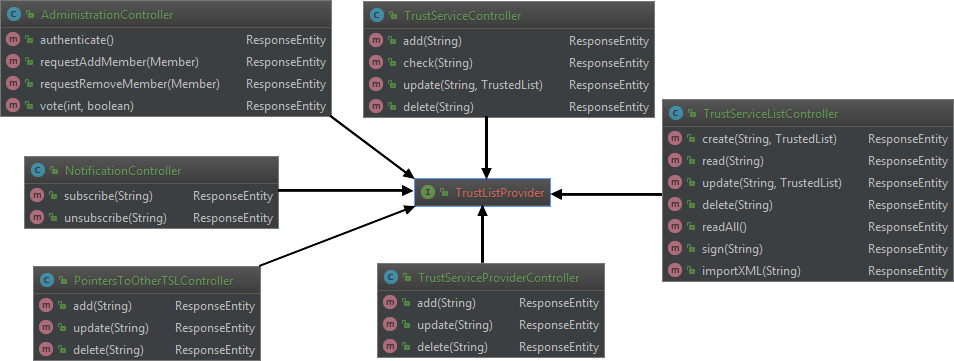
\includegraphics[scale=0.73]{figures/rest-controllers}
	\caption{Contrôleurs exposés par le Trust List Provider}
	\label{fig:rest-controllers}
\end{figure}

Les contrôleurs définis dans la Figure~\ref{fig:rest-controllers} sont détaillés ci-dessous:
\begin{itemize}
	\item Le contrôleur \textit{Administration} permet aux administrateurs de s'authentifier pour ensuite pouvoir gérer les utilisateurs;
	\item Le contrôleur \textit{Notification} permet aux utilisateurs de s'abonner et de se désabonner des TSLs;
	\item Le contrôleur \textit{PointersToOtherTSL} permet aux administrateurs de gérer les pointeurs vers les autres TSLs;
	\item Le contrôleur \textit{TrustServiceList} permet à tous les utilisateurs de lire une TSL particulière ou toutes les TSLs, et permet aux administrateurs de créer, éditer, supprimer, signer ou importer une TSL;
	\item Le contrôleur \textit{TrustServiceProvider} permet aux administrateurs d'ajouter, éditer ou retirer un TSP d'une TSL.
	\item Le contrôleur \textit{TrustService} permet aux administrateurs d'ajouter, éditer ou retirer un TS d'un TSP, et permet à tous les utilisateurs de vérifier un TS en fonction de critères de filtrage.
\end{itemize}

\section{Validation de la solution}

Durant ce stage, plusieurs méthodes de validation ont été mises en place. 
Étant donné que le projet est encore en cours de réalisation au moment de la rédaction de ce mémoire, le processus de validation ne peut être considéré comme complet. Cependant, nous avons tout de même mis en place plusieurs mesures de vérification, dans le but d'attester de la conformité des travaux effectués avec les besoins initiaux présentés au Chapitre~\ref{chap:prob}.

Dans un premier temps, la première validation a consisté à valider les choix opérés à la suite de l'état de l'art en début de stage. Cette étape a été très importante car c'est elle qui nous a permis de valider les technologies à utiliser dans le projet. Pour cela, j'ai réalisé une preuve de concept permettant d'interfacer les technologies Ethereum et IPFS dans le but de stocker des données dans un environnement décentralisé et distribué. Cette preuve de concept a ensuite fait l'objet d'une démonstration à l'équipe de projet qui a pu valider l'utilisation des technologies sur la base du travail que j'ai réalisé.

Ensuite, d'autres points de validation ont eu lieu durant le stage. Tous les jours, une réunion rapide a été organisée afin de prendre connaissance du travail réalisé et restant pour chaque membre de l'équipe. Cette réunion qui s'inscrit dans la méthodologie Scrum permet de connaître l'avancement du projet pour chaque membre et permet aussi de mettre en avant les difficultés rencontrées ou de recevoir des validations orales et informelles dans nos choix d'implémentation. 

Toujours dans la méthodologie Scrum, à chaque fin de sprint est organisée une réunion. Elle a pour but de faire le bilan des tâches réalisées durant les deux semaines de sprint et d'engager le nouveau sprint. Par ailleurs, elle permet de faire le point sur l'amélioration continue du processus de gestion de projet et de la réalisation des tâches afin de toujours augmenter la performance de l'équipe. 

Une autre validation spécifique à ce projet est la conformité au standard ETSI TS 119 612~\cite{ETSITS119612}. En effet, tout au long du stage il a été important et nécessaire de se référer régulièrement à ce standard puisque l'exigence première du projet est d'être conforme à celui-ci. Il a donc été nécessaire de faire valider chaque module en s'appuyant sur le standard lors de la phase de recherche, afin de s'assurer que la direction choisie permettait d'aboutir à une fonctionnalité valide.

Enfin, la validation a aussi porté sur l'aspect technique. Au fur et à mesure de l'avancée du projet, des tests unitaires et d'intégration ont été mis en place afin de valider les différentes fonctionnalités du service de gTSL.

\chapter{Résultats obtenus \& Perspectives}

Les résultats définitifs du stage sont à l'heure actuelle inconnus puisque la date de livraison est prévue pour le 30 novembre 2017. Malgré cela, tous les retours du consortium d'entreprises du projet FutureTrust ont été jusqu'à présent positifs vis-à-vis du travail réalisé par l'équipe notamment concernant les documents de conception et les choix opérés. De plus, il y a un fort enthousiasme autour de la gTSL de par l'utilisation de la blockchain dans un projet européen.

Un autre point à soulever concernant ce projet est que c'est un projet de recherche et développement. Cela signifie que la Commission Européenne attend de l'innovation dans la conception et la réalisation tout en conservant une simplicité d'utilisation pour les utilisateurs finaux. Le challenge a donc été d'adapter une technologie récente et complexe qu'est la blockchain à un système existant. Notre objectif est que ce projet rencontre un grand succès afin qu'il soit adopté par la Commission Européenne pour remplacer l'architecture actuelle.

Un des résultats préliminaires du projet est la démonstration de notre capacité à utiliser la blockchain dans le cadre du projet FutureTrust suite à la preuve de concept que j'ai réalisée. Cette étape a eu lieu après que l'équipe ait validé les choix technologiques que j'ai proposés à la suite de l'état de l'art. À ce moment, le consortium a commencé à s'intéresser à notre conception de la gTSL et à sa mise en place imminente. J'ai donc rédigé un document explicatif de l'utilisation de la blockchain dans le cadre de la gTSL. Ce document s'intitule Integration of Ethereum \& IPFS et est disponible en Annexe~\ref{anx:ipfs-ethereum}. À la suite de la lecture de ce document, un membre de l'ETSI a montré un très grand intérêt pour notre travail et a invité l'équipe à venir présenter ce papier à un atelier blockchain qui aura lieu début 2018 au Luxembourg.

\chapter{Conclusion}

Ce stage de fin d'études vient conclure la formation de trois ans que j'ai suivie à Télécom Nancy. Cette formation m'a fait acquérir un grand nombre de compétences et connaissances techniques, que j'ai pu restituer tout au long de ce stage. Ces études m'ont aussi apporté des qualités humaines telles que la gestion du stress, l'évolution en équipe ou encore la logique de raisonnement, et cela notamment grâce aux nombreux projets qui ont été réalisés jusque maintenant.

Après avoir eu l'occasion d'étudier et d'exploiter la technologie blockchain pendant ce stage, je résumerais les défis de notre étude par les points suivants. Dans un premier temps, l'émergence de la blockchain a réellement bouleversé l'économie mondiale et a amené une prise de conscience générale des limites des systèmes centralisés. Aujourd'hui et plus que jamais, les entreprises sont intéressées par la mise en place d'architectures reposant sur la blockchain et plus particulièrement le secteur bancaire qui ne veut pas rater le virage des crypto-monnaies. Le problème persistant actuellement est le manque de régulation de cette technologie, plusieurs pays prévoient d'établir des réglementations autour de la blockchain et de la crypto-monnaie dans les années à venir.

En ce sens, l’initiative du projet FutureTrust quant à l'innovation autour de la confiance électronique à l'échelle mondiale est une excellente idée. 
Ce projet de recherche et développement ayant pour objectif de mettre en application le règlement de l'Union Européenne sur l'identification électronique et les services de confiance pour les transactions électroniques sécurisées au sein de l'UE a été une réelle opportunité de promouvoir la blockchain.
En effet, l'Europe souhaite être un acteur majeur et un pionnier de l'utilisation de cette technologie. À ce titre, elle joue un rôle clé dans son développement.
Malgré cela, une grande nécessité de communication autour de cette technologie persiste, car sa complexité peut freiner l'innovation et à terme entraîner sa disparition.
Il est vrai qu'au premier abord, la blockchain est un concept flou et complexe car son fonctionnement est difficilement compréhensible pour un non initié à l'informatique et à la cryptographie.
Le challenge pour les années futures se trouve dans la démocratisation de cette technologie par la mise en place de services grand public ergonomiques et simples d'utilisation.
Le projet réalisé dans le cadre de ce stage propose une première approche d'intégration d'une blockchain au sein d'un service européen. De plus, l'engouement du consortium de FutureTrust, concernant les résultats déjà obtenus, est très encourageant pour la suite.

À titre personnel, ce projet a été un immense défi de par son innovation, sa complexité et sa portée. Sa réalisation a demandé de la réflexion, des remises en question et de la force de proposition car j'ai été amené à résoudre des problèmes techniques et scientifiques concernant les architectures décentralisées et l'intégration de la technologie blockchain.
De plus, je suis convaincu que cette technologie est l’avenir du numérique et que les solutions à venir, particulièrement dans le secteur bancaire, vont créer une réelle rupture technologique.
J’ai par ailleurs décidé de poursuivre ce projet dans l'entreprise Ar{\texteta}s afin de participer à l'élaboration du service de liste de confiance globale jusqu'à sa livraison et de continuer de concevoir des projets innovants autour de la blockchain.

\cleardoublepage
\renewcommand{\tocbibname}{Bibliographie / Webographie}
\bibliography{example} % See example.bib 
\bibliographystyle{plain}

\listoffigures

\lstlistoflistings

\chapter*{Acronymes}
\addcontentsline{toc}{chapter}{Acronymes}

\begin{enumerate}
	\item \textbf{API} - Application Programming Interface
	\item \textbf{BFT} - Byzantine Fault Tolerant
	\item \textbf{BPMN} - Business Process Model and Notation
	\item \textbf{dApp} - decentralized Application
	\item \textbf{eIDAS} - services de confiance pour les transactions électroniques sécurisées au sein de l'UE
	\item \textbf{ESN} - Entreprise de Services du Numérique
	\item \textbf{ETH} - ETHer
	\item \textbf{ETSI} - European Telecommunications Standards Institute
	\item \textbf{EVM} - Ethereum Virtual Machine
	\item \textbf{gTSL} - Global Trust Service status List
	\item \textbf{HTTP} - HyperText Transfer Protocol 
	\item \textbf{ICO} - Initial Coin Offering
	\item \textbf{IPFS} - InterPlanetary File System
	\item \textbf{JSON} - JavaScript Object Notation
	\item \textbf{KSI} - Keyless Signature Infrastructure
	\item \textbf{LoTL} - List of The Lists
	\item \textbf{REST} - REpresentational State Transfer
	\item \textbf{TS} - Trust Services
	\item \textbf{TSL} - Trust Service Lists
	\item \textbf{TSP} - Trust Service Providers
	\item \textbf{UE} - Union Europénne
	\item \textbf{UML} - Unified Modeling Language
	\item \textbf{URI} - Uniform Resource Identifier
	\item \textbf{URL} - Uniform Resource Locator
	\item \textbf{XML} - eXtensible Markup Language
\end{enumerate}

\chapter*{Glossaire}
\addcontentsline{toc}{chapter}{Glossaire}

\begin{enumerate}
	\item \textbf{attaque Sybil}: Une attaque Sybil est une attaque informatique qui vise à renverser un système par la création de fausses identités dans un réseau pair-à-pair.
	\item \textbf{Bitcoin}: Bitcoin est une crypto-monnaie et un système de paiement pair-à-pair.
	\item \textbf{cluster}: Un cluster est un ensemble de serveurs sur un réseau qui agissent dans un but commun.
	\item \textbf{crypto-monnai}e: La crypto-monnaie aussi appelée monnaie cryptographique est une monnaie électronique basé sur les principes de la cryptographie.
	\item \textbf{design pattern}: Un design pattern, appelé patron de conception en français, est un modèle considéré comme bonne pratique en réponse à un problème de conception d'un logiciel.
	\item \textbf{framework}: Un framework est un ensemble de composants développées par un tierce permettant de définir une architecture logicielle.
	\item \textbf{hash}: Un hash est le résultat d'une fonction de hachage qui permet d'identifier rapidement une donnée.
	\item \textbf{logging}: Le logging est un dispositif permettant de stocker un historique des évènements attachés à un processus.
	\item \textbf{minage}: Le minage est aussi un moyen de sécuriser le réseau en créant, vérifiant, publiant et propageant les blocs dans la blockchain.
	\item \textbf{newsletter}: Une newsletter, appelé lettre d'information en français, est un document d'information transmis par courrier électronique à l'ensemble des abonnés qui y ont souscrit.
	\item \textbf{pair-à-pair}: Le pair-à-pair est un modèle de réseau informatique similaire au modèle client-serveur mais où chaque client est aussi un serveur.
	\item \textbf{point individuel de défaillance}: Un point individuel de défaillance, appelée single point of failure en anglais, est un point d'un système informatique dont le reste du système est dépendant et dont une panne entraîne l'arrêt complet du système.
	\item \textbf{scrum meeting}: Un scrum meeting, communément appelé mêlée en français, est une réunion courte et énergique faisant partie de la méthodologie Scrum, qui permet à l'équipe de discuter de l'avancée d'un sprint et de lever les points bloquants du projet.
	\item \textbf{smart contract}: Les smart contracts, appelés contrats intelligents en français, permettent d'échanger de l'argent, des biens, des parts ou n'importe quel actif de manière transparente, sans conflits et en évitant tout service intermédiaire.
	\item \textbf{sprint}: Un sprint est une période sur laquelle sont réalisées des tâches définies.
	\item \textbf{timestamping}: Le timestamping, appelé horodatage en français, est un mécanisme qui consiste à associer une date et une heure à un événement, une information ou une donnée informatique.
	\item \textbf{Uber}: Uber est l'entreprise qui déclencha ce qu'on appelle l'ubérisation.
	\item \textbf{ubérisation}: L'ubérisation est un phénomène économique désignant l'utilisation de services permettant aux professionnels et aux clients de se mettre en contact direct grâce à l'utilisation des nouvelles technologies.
	\item \textbf{ubériser}: Ubériser est le verbe issu du substantif ubériser.
	\item \textbf{web service}: Un web service correspond à l'implémentation d'une ressource identifiée par une URL.
\end{enumerate}

\cleardoublepage
\renewcommand{\thesubsection}{\Roman{subsection}}

\appendix
\part*{Annexes}
\addcontentsline{toc}{part}{Annexes}
\clearpage

\chapter{Document de synthèse - Integration of Ethereum \& IPFS}
\label{anx:ipfs-ethereum}
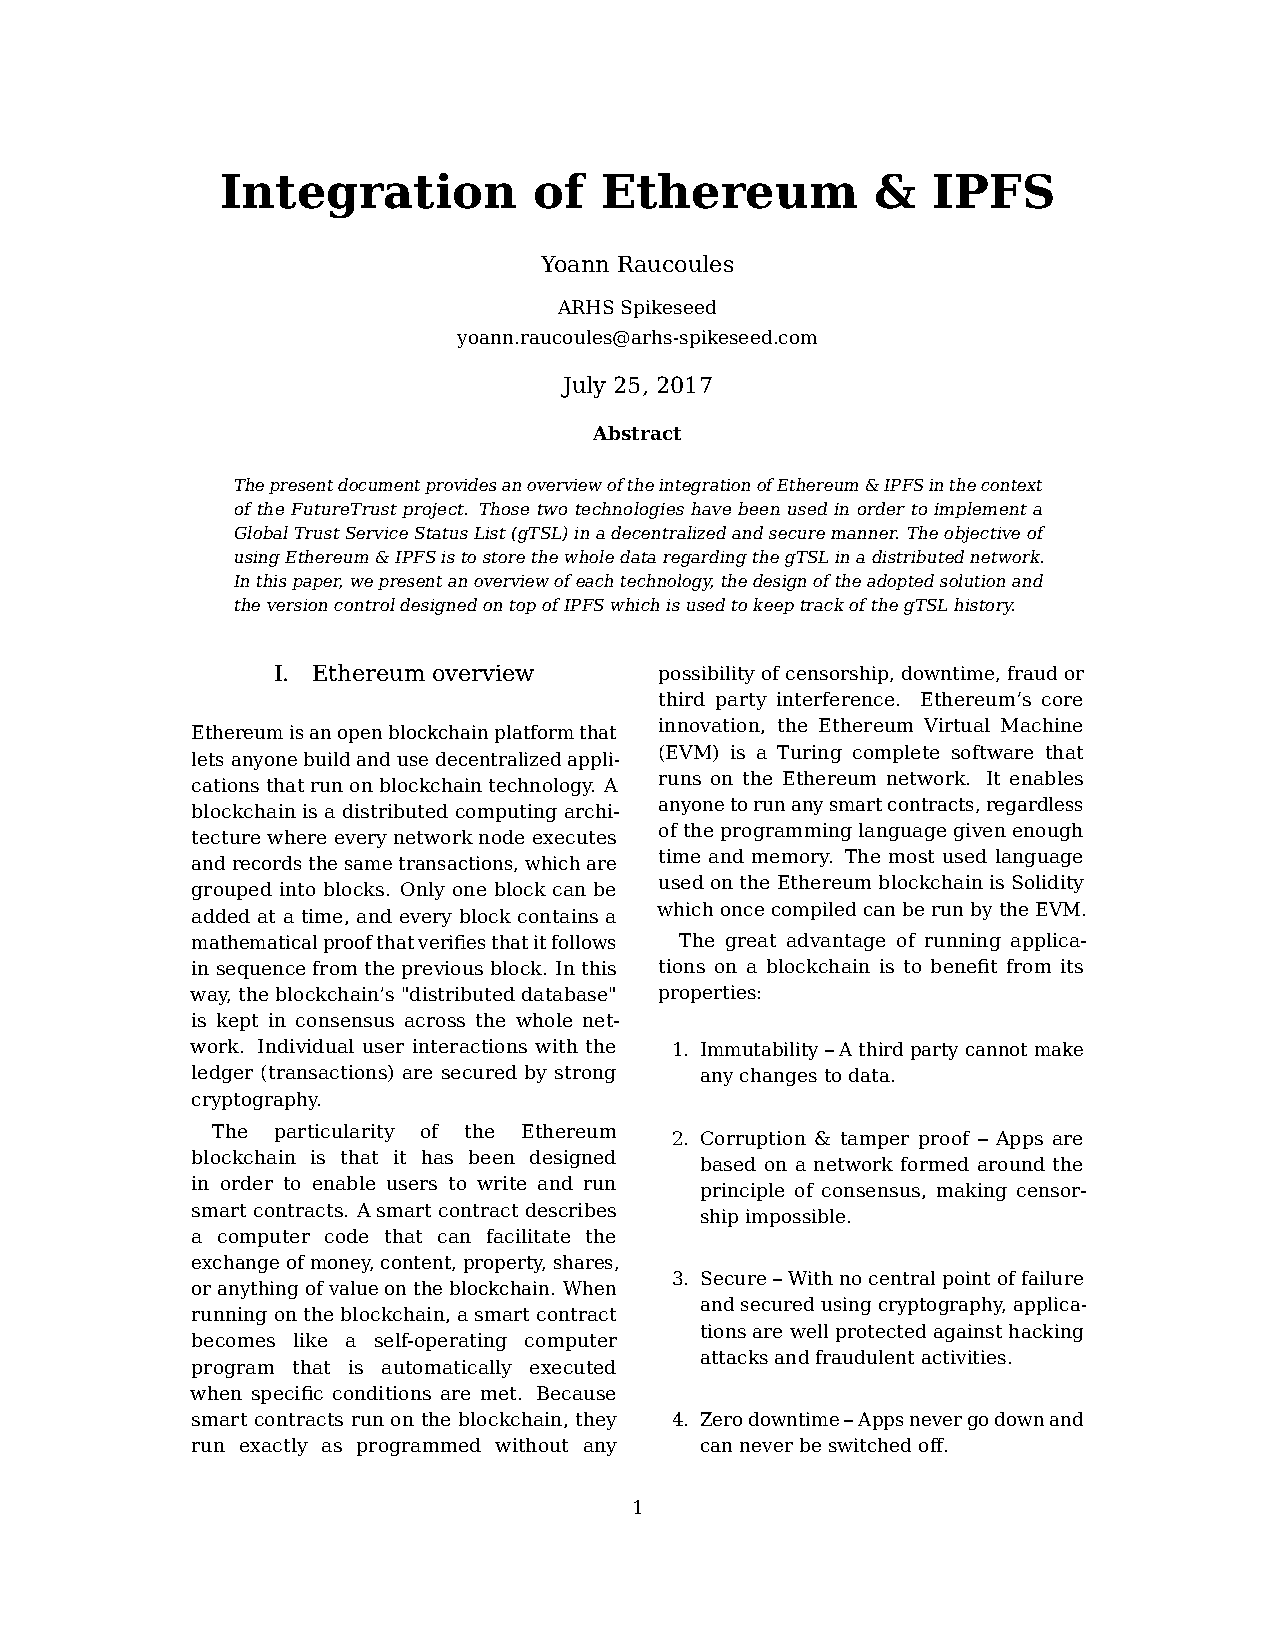
\includepdf[pages=-]{pdf/ipfs-ethereum.pdf}
\clearpage

\chapter{Analyse - gTSL Search Engine}
\label{anx:gtsl-search-engine}
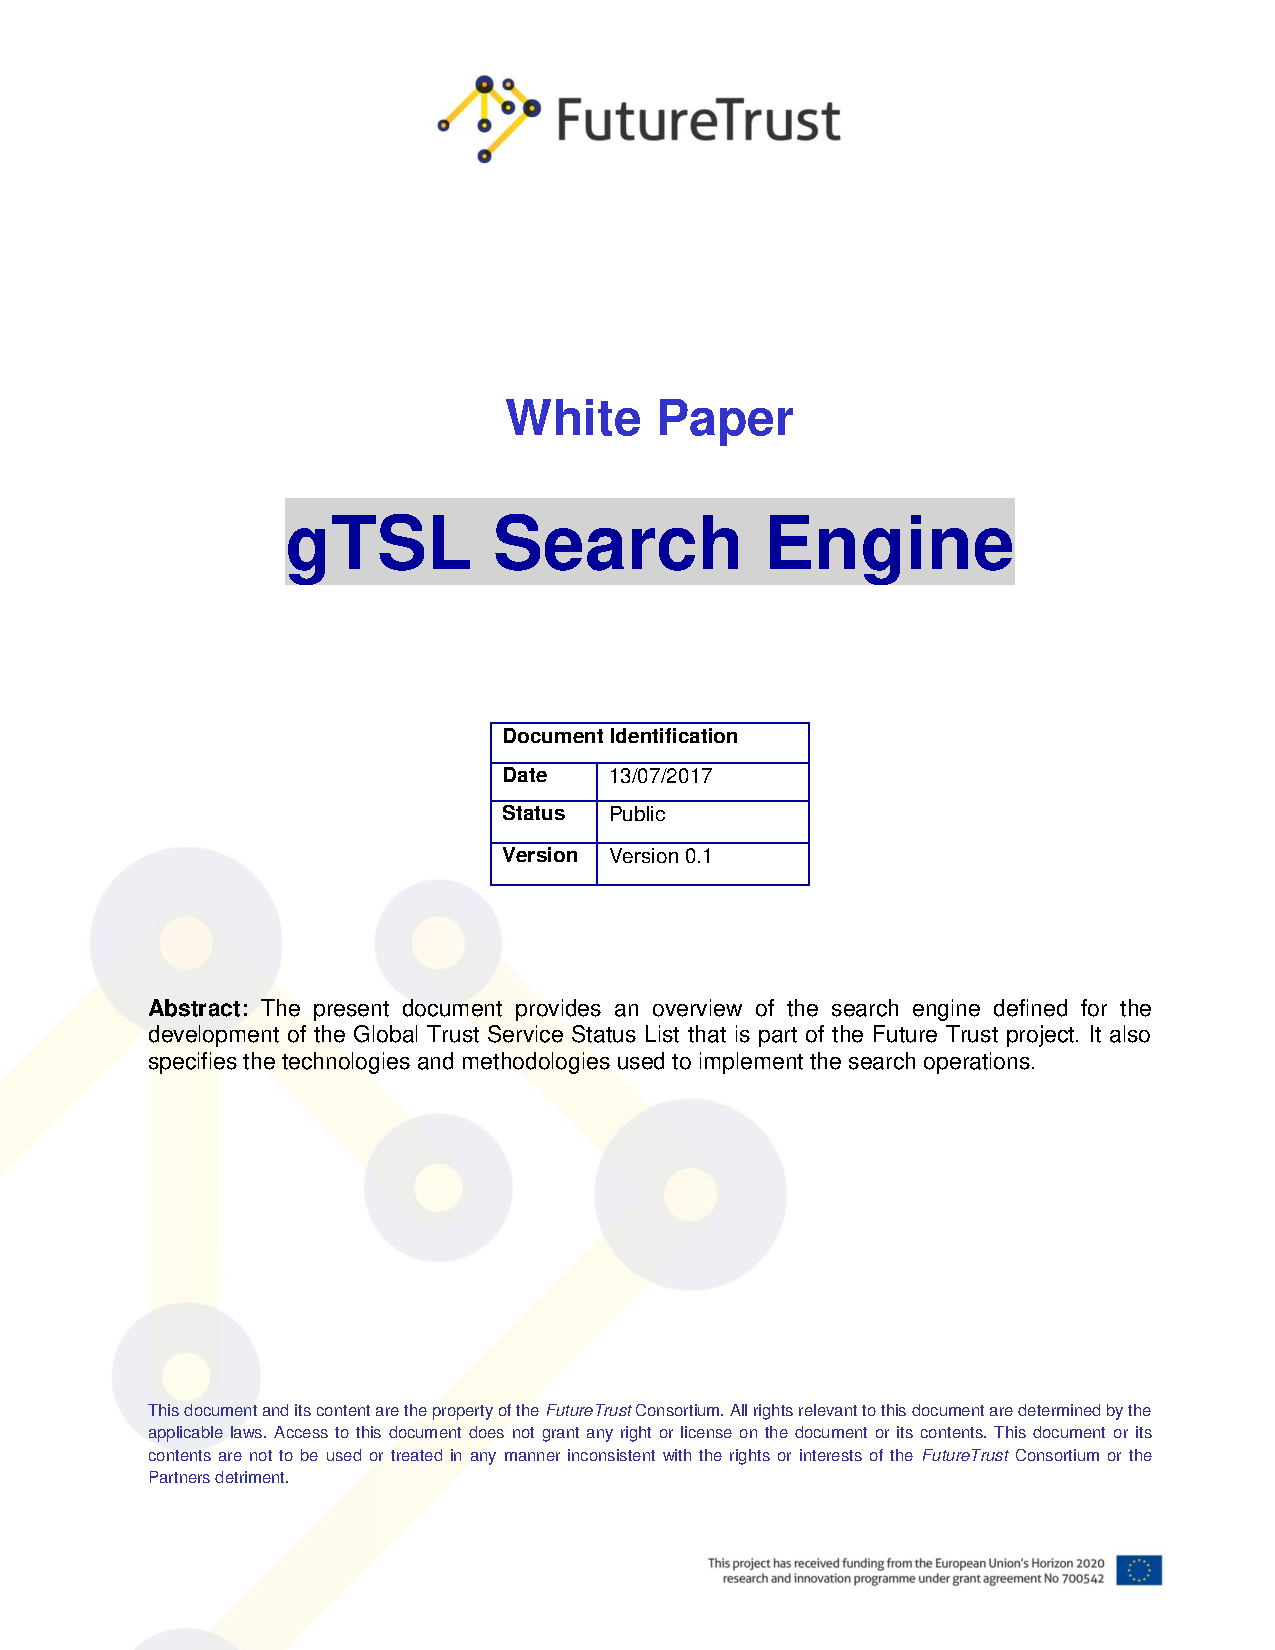
\includepdf[pages=-]{pdf/gtsl-search-engine.pdf}
\clearpage

\chapter{Documentation - gTSL - Project Setup Documentation}
\label{anx:gtsl-setup}
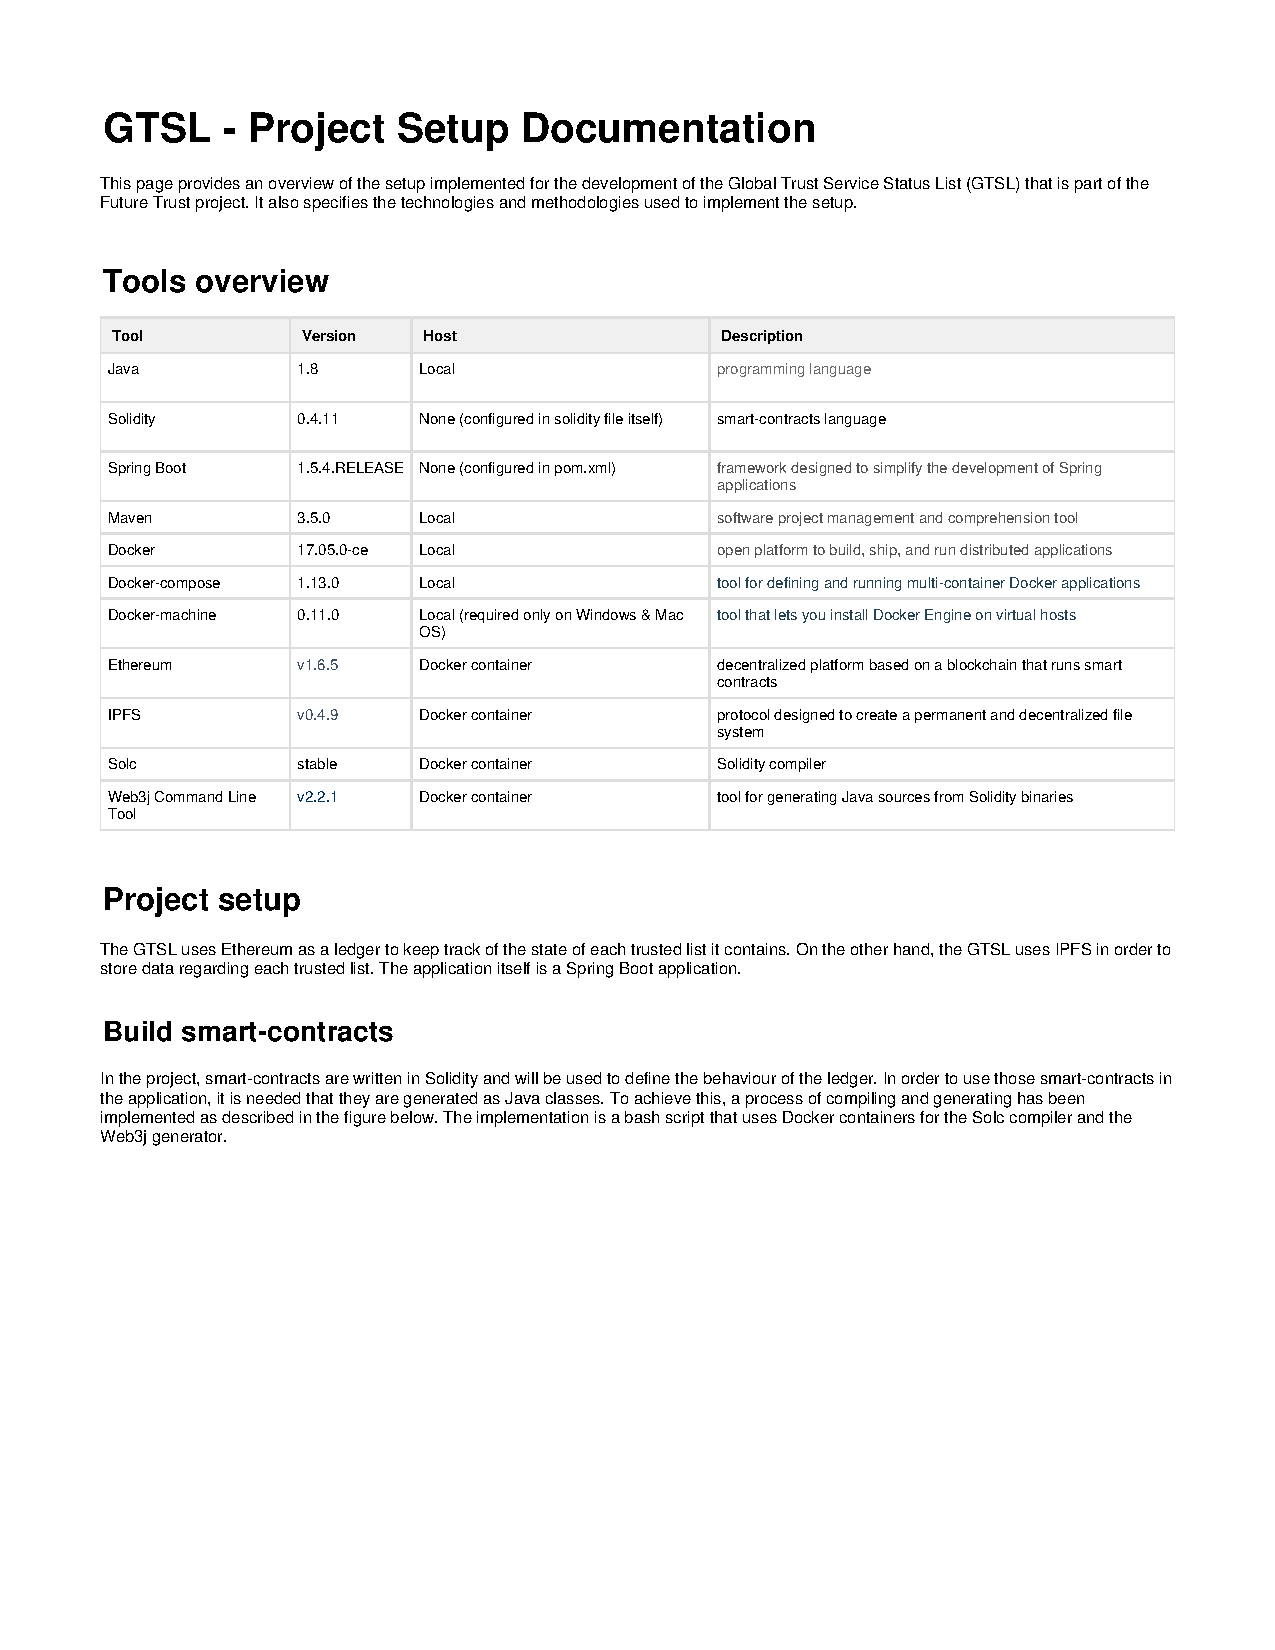
\includepdf[pages=-]{pdf/gtsl-setup.pdf}
\clearpage

\chapter{Documentation - gTSL - Project Setup Guidelines}
\label{anx:gtsl-guidelines}
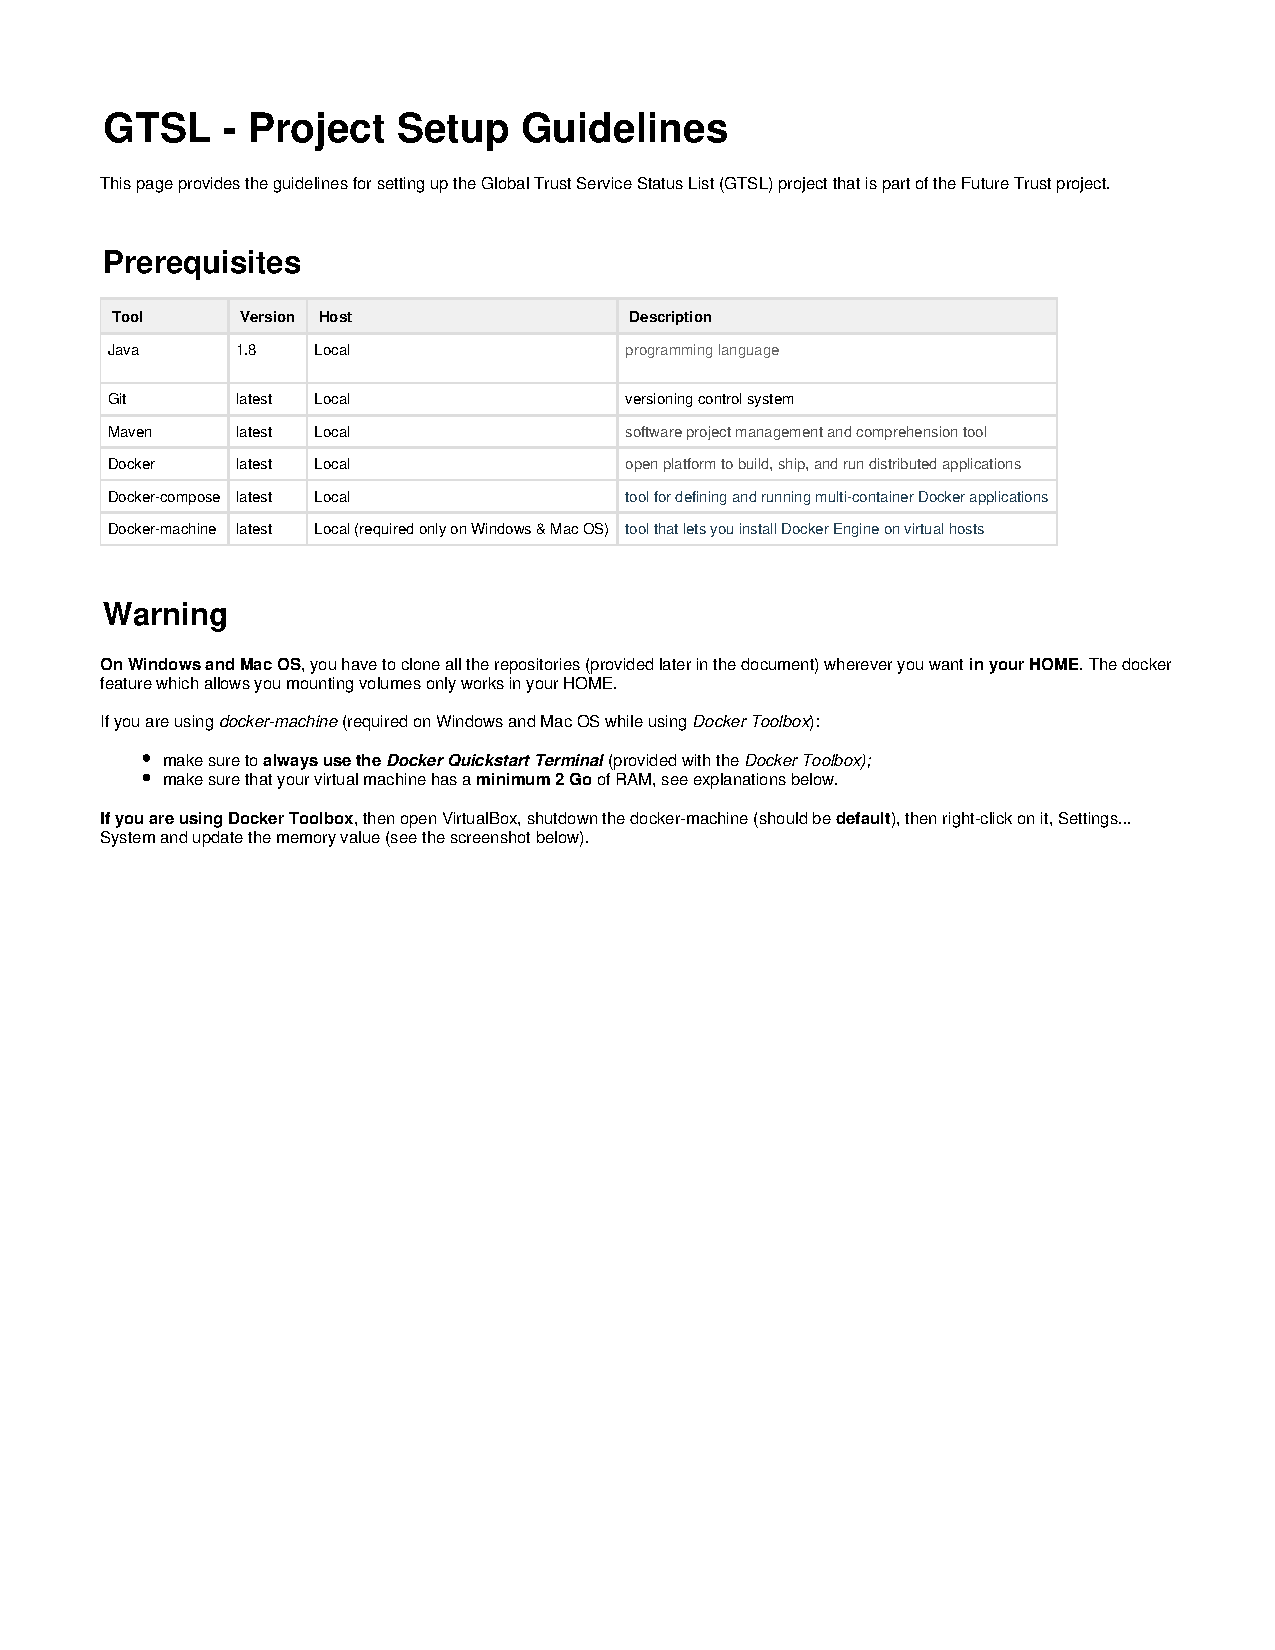
\includepdf[pages=-]{pdf/gtsl-guidelines.pdf}
\clearpage

\chapter{Analyse - Comparaison des technologies}
\label{anx:comparison}

\begin{figure}[h]
	\centering
	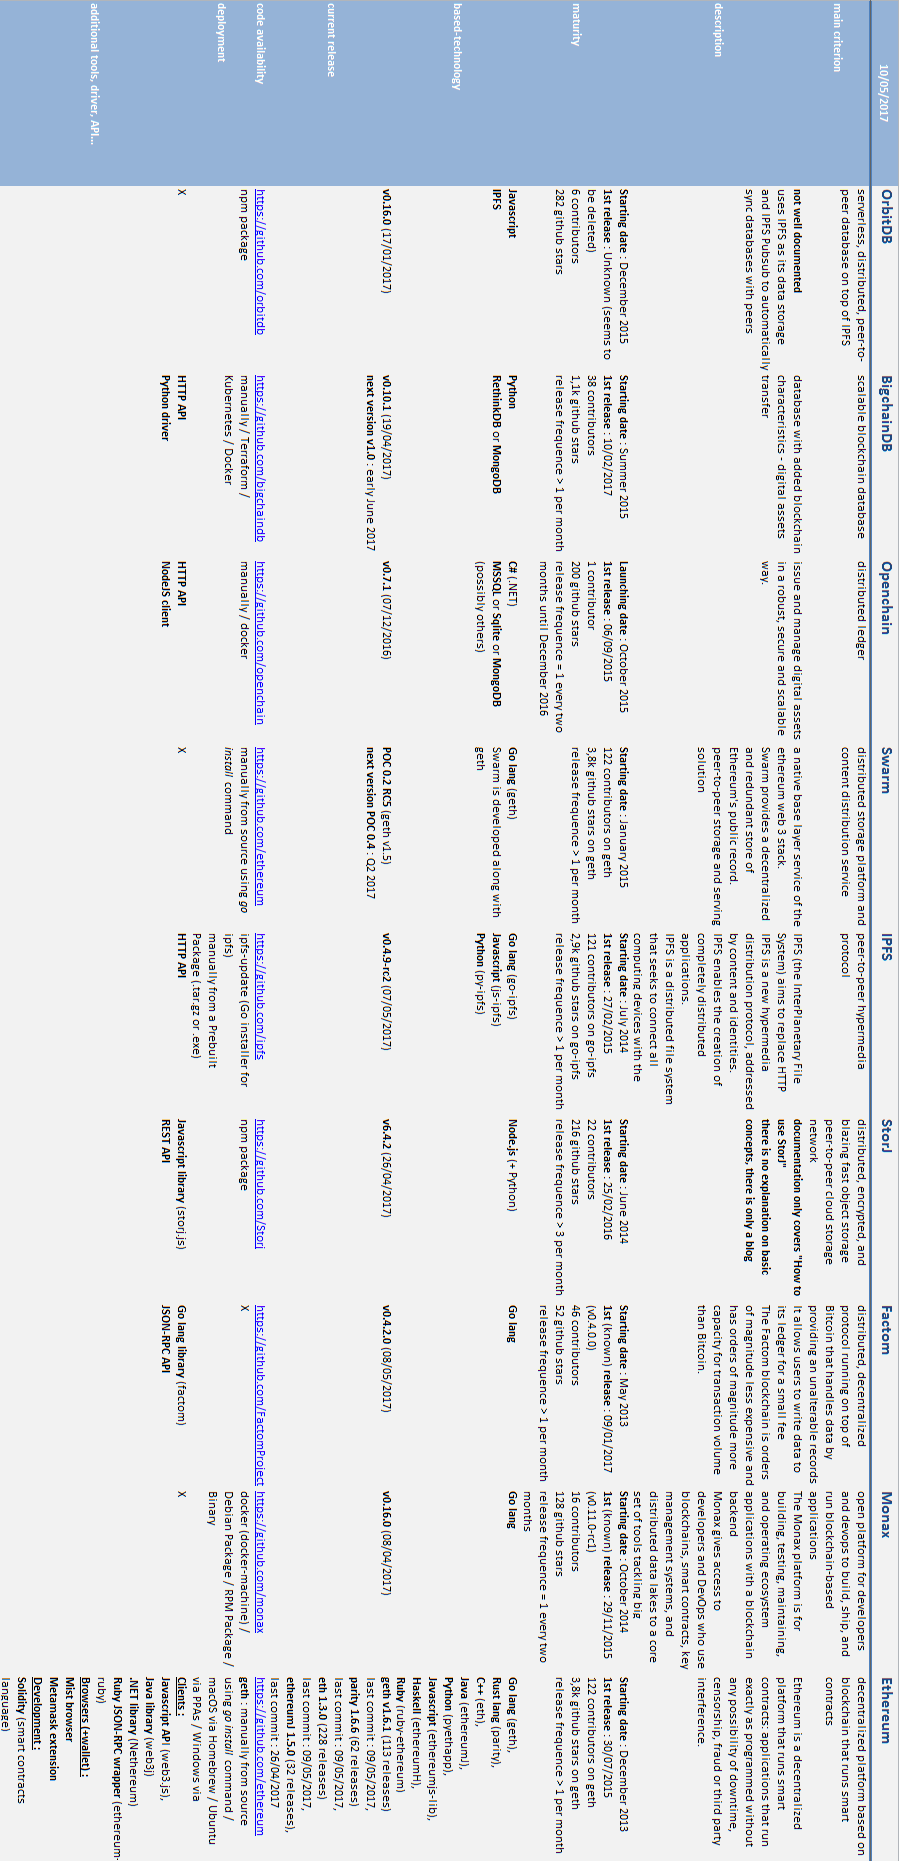
\includegraphics[scale=0.5]{figures/blockchain-technologies-comparison-part1}
	\caption{Comparaison des technologies - Partie 1}
	\label{fig:comparison-part1}
\end{figure}

\begin{figure}[h]
	\centering
	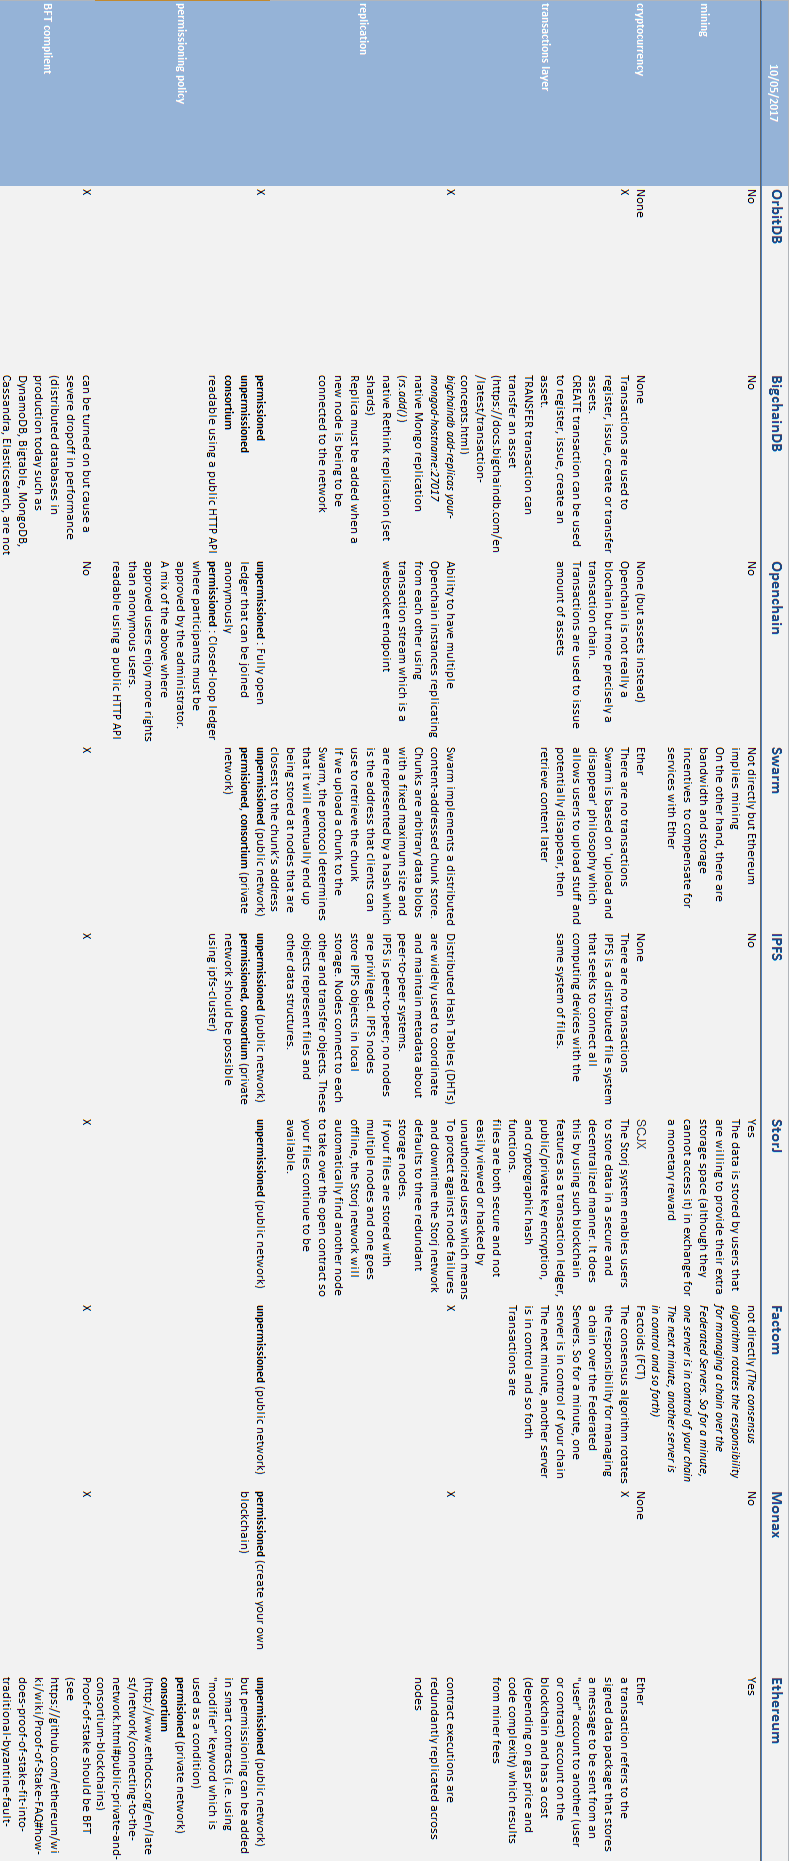
\includegraphics[scale=0.5]{figures/blockchain-technologies-comparison-part2}
	\caption{Comparaison des technologies - Partie 2}
	\label{fig:comparison-part2}
\end{figure}

\begin{figure}[h]
	\centering
	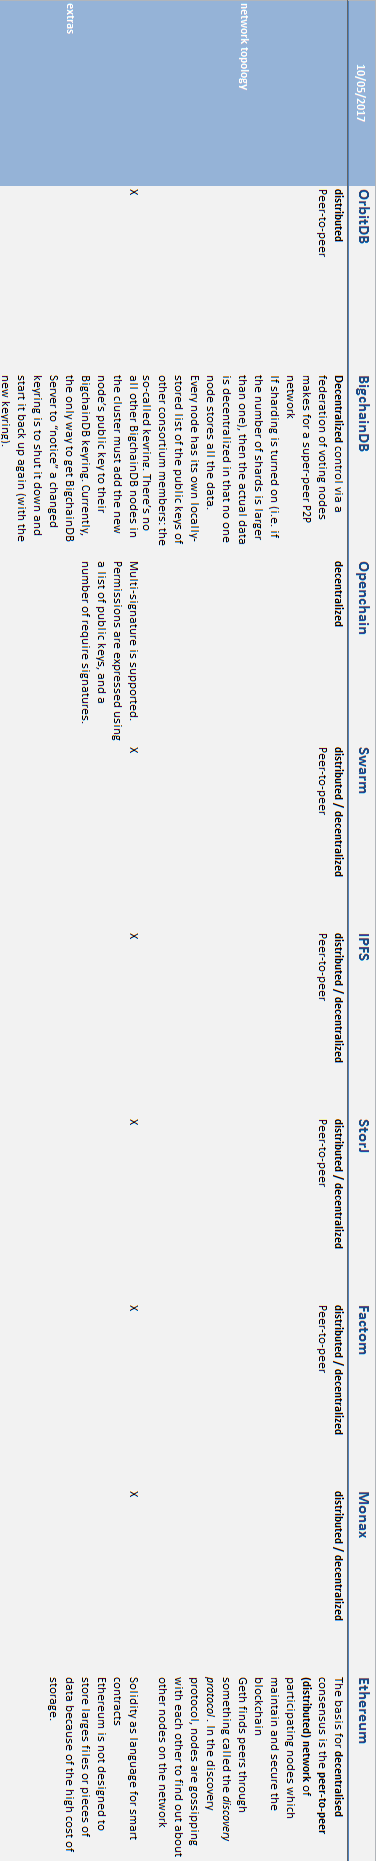
\includegraphics[scale=0.5]{figures/blockchain-technologies-comparison-part3}
	\caption{Comparaison des technologies - Partie 3}
	\label{fig:comparison-part3}
\end{figure}

\cleardoublepage
\thispagestyle{empty}

\section*{Résumé}
\addcontentsline{toc}{chapter}{Résumé}

La technologie blockchain s'est popularisée ces dernières années et devrait être largement utilisée dans un futur proche. Malgré l'attention considérable et médiatique, seulement quelques produits exploitent tout le potentiel de cette technologie (e.g., Bitcoin and Ethereum). Pourtant, les propriétés innovantes qu'apporte la blockchain en font un outil idéal pour concevoir des architectures de sécurité.
\\
La Commission européenne a lancé un projet, nommé FutureTrust, pour aborder les mesures présentées dans
son règlement sur l'identification électronique (eID) et les services de confiance pour les transactions électroniques sécurisées au sein de l'UE (eIDAS). Le consortium FutureTrust se compose de seize partenaires, dont ARHS Spikeseed, qui sont engagés dans la conception et la mise en œuvre de solutions pour faire appliquer le règlement eIDAS.
\\
Le présent document détaille l'implémentation d'un service de liste de confiance globale basé sur la blockchain. Plus particulièrement, il présente la révision de l’architecture actuelle des listes de confiance, décrit l'implémentation de cette nouvelle architecture, et expose les avantages de l'utilisation d'une blockchain dans le contexte de la confiance numérique. Le service développé a pour rôle de gérer des listes de confiance conforme au standard ETSI 119 612 et de permettre à toute partie intéressée de déterminer si un service de confiance respecte les exigences du standard. D'un point de vue technique, le système mis en place a pour vocation de stocker des données relatives à la confiance numérique dans un registre public immuable. Le système utilise un réseau pair-à-pair décentralisé et distribué, assurant l'intégrité et la disponibilité des informations ainsi qu'une résilience forte contre les attaques par déni de service.

{\bf Mots-clés : eIDAS, blockchain, décentralisation, confiance numérique} 


\section*{Abstract}
\addcontentsline{toc}{chapter}{Abstract}

Blockchain technology emerged over the last few years and should be widely deployed in the near future. Despite the considerable amount of interest and media attention, only a few products exploit the full potential of this technology (e.g., Bitcoin and Ethereum). However, the innovative properties of blockchain make it an ideal tool for devising novel security architectures. 
\\
The European Commission initiated a project, denominated FutureTrust, to address the measures introduced in its regulation on electronic identification (eID) and trusted services for electronic transactions in the internal market (eIDAS). FutureTrust's consortium consists of sixteen partners, including ARHS Spikeseed, which are engaged in the design and implementation of solutions to enforce the eIDAS regulation. 
\\
The present document specifies the requirements for a blockchain-based global trusted lists management service. More specifically, it introduces the redesign of the current architecture for trusted lists, describes the implementation of this novel architecture, and discusses the advantages of the use of blockchain in the context of digital trust. The developed service aims at managing trusted lists in compliance with ETSI 119 612 and enables any interested party to determine whether a trust service is or was operating in compliance with the relevant requirements. Technically, the system we implemented is used for storing data related to digital trust in an immutable public ledger. The system uses a peer-to-peer decentralized and distributed network, guarantees integrity and availability of information, and improves resilience against denial of service attacks.

{\bf Keywords : eIDAS, blockchain, decentralization, digital trust}

\end{document}
